% Project report, Mangalore Institute of Technology & Engineering, Dept. of AI & ML.
% Build: report/build.sh   (renders the Mermaid diagrams, then pdflatex + bibtex)
\documentclass[12pt,a4paper,oneside]{report}

\usepackage[T1]{fontenc}
\usepackage[utf8]{inputenc}
\usepackage{mathptmx}                       % Times for text and maths
\usepackage[scaled=0.9]{helvet}
\usepackage{microtype}
\usepackage[a4paper,left=1.3in,right=1.05in,top=1.15in,bottom=1.1in,headsep=16pt,footskip=26pt]{geometry}
\usepackage{setspace}
\usepackage{amsmath,amssymb}
\usepackage{graphicx}
\usepackage{xcolor}
\usepackage{booktabs,array,tabularx,longtable,multirow}
\usepackage{colortbl}
\usepackage{caption}
\usepackage{float}
\usepackage{placeins}
\usepackage{enumitem}
\usepackage{pdflscape}
\usepackage{fancyhdr}
\usepackage{eso-pic}
\usepackage{titlesec}
\usepackage{tocloft}
\usepackage{listings}
\usepackage{algorithm}
\usepackage{algpseudocode}
\usepackage{tikz}
\usetikzlibrary{arrows.meta,positioning,shapes.geometric,calc,fit,backgrounds}
\usepackage[hidelinks,bookmarksnumbered]{hyperref}

% Everything that names a person or a course lives here, so it is filled in once.
% Lines marked CHECK were copied from the department's reference report; confirm them with your guide.

\newcommand{\ProjectTitle}{Probabilistic Cascading Failure and Agent Assisted Root Cause Analysis for Microservice Systems}
\newcommand{\CourseLine}{23AISE409 PROJECT PHASE -- II}   % CHECK: course code and phase
\newcommand{\AcademicYear}{2026--2027}

% Students in USN order, as in the department's reference report.
\newcommand{\StudentOne}{ANISH C}
\newcommand{\USNOne}{4MT23AI008}
\newcommand{\StudentTwo}{ROYSON SALIS}
\newcommand{\USNTwo}{4MT23AI046}
\newcommand{\StudentThree}{DHANUSH K MURTHY}
\newcommand{\USNThree}{4MT23AI401}
\newcommand{\StudentFour}{K BHARATH PARMAR}
\newcommand{\USNFour}{4MT24AI402}

\newcommand{\GuideName}{Dr. Manjunath Prasad H R}   % CHECK: the project slide calls him Head of Department; the department's reference report lists him as guide, Assistant Professor
\newcommand{\GuideDesignation}{Assistant Professor}
\newcommand{\HODName}{Dr. Sunil Kumar S}       % CHECK
\newcommand{\PrincipalName}{Dr. Prashanth C M} % CHECK

\graphicspath{{figures/}{diagrams/}}

% ---- layout -------------------------------------------------------------
\onehalfspacing
\setlength{\parindent}{0pt}
\setlength{\parskip}{6pt}
\setlist{itemsep=2pt,topsep=4pt,parsep=2pt}
\renewcommand{\topfraction}{0.92}\renewcommand{\bottomfraction}{0.85}
\renewcommand{\textfraction}{0.07}\renewcommand{\floatpagefraction}{0.6}
\setcounter{topnumber}{3}\setcounter{bottomnumber}{2}\setcounter{totalnumber}{5}
\setlength{\textfloatsep}{14pt plus 4pt minus 4pt}\setlength{\floatsep}{12pt plus 3pt minus 3pt}\setlength{\intextsep}{12pt plus 3pt minus 3pt}

% double-line border on every page (outer heavy, inner light)
\AddToShipoutPictureBG{%
  \begin{tikzpicture}[remember picture,overlay]
    \draw[line width=1.3pt] ($(current page.north west)+(0.5in,-0.5in)$) rectangle ($(current page.south east)+(-0.5in,0.5in)$);
    \draw[line width=0.4pt] ($(current page.north west)+(0.56in,-0.56in)$) rectangle ($(current page.south east)+(-0.56in,0.56in)$);
  \end{tikzpicture}}

\pagestyle{fancy}
\fancyhf{}
\renewcommand{\headrulewidth}{0.4pt}
\fancyhead[L]{\small\itshape\nouppercase{\leftmark}}
\fancyhead[R]{\small Phase II Project Report}
\fancyfoot[L]{\footnotesize Dept.\ of AI \& ML, MITE Mangalore}
\fancyfoot[R]{\footnotesize \AcademicYear}
\fancyfoot[C]{\small Page \thepage}
\fancypagestyle{plain}{\fancyhf{}\renewcommand{\headrulewidth}{0pt}\fancyfoot[L]{\footnotesize Dept.\ of AI \& ML, MITE Mangalore}\fancyfoot[R]{\footnotesize \AcademicYear}\fancyfoot[C]{\small Page \thepage}}

% chapter and section headings as in the department's reports
\titleformat{\chapter}[display]{\centering\bfseries\fontsize{16}{20}\selectfont}{CHAPTER \thechapter}{8pt}{\fontsize{16}{20}\selectfont\MakeUppercase}
\titlespacing*{\chapter}{0pt}{-10pt}{22pt}
\titleformat{\section}{\bfseries\fontsize{13}{16}\selectfont}{\thesection}{0.6em}{}
\titleformat{\subsection}{\bfseries\fontsize{12}{15}\selectfont}{\thesubsection}{0.6em}{}
\titleformat{\subsubsection}{\bfseries\itshape\fontsize{12}{15}\selectfont}{\thesubsubsection}{0.6em}{}
\titlespacing*{\section}{0pt}{14pt}{4pt}
\titlespacing*{\subsection}{0pt}{10pt}{3pt}
\titlespacing*{\subsubsection}{0pt}{8pt}{2pt}

% numbering per chapter: Figure 3.1, Table 3.4, Listing 5.2, Algorithm 5.1
\captionsetup{font=small,labelfont=bf,labelsep=colon,skip=6pt}
\captionsetup[table]{position=above}
\captionsetup[figure]{position=below}
\renewcommand{\thefigure}{\thechapter.\arabic{figure}}
\renewcommand{\thetable}{\thechapter.\arabic{table}}
\renewcommand{\thealgorithm}{\thechapter.\arabic{algorithm}}
\makeatletter
\@addtoreset{figure}{chapter}\@addtoreset{table}{chapter}\@addtoreset{algorithm}{chapter}
\makeatother

% contents, lists
\renewcommand{\cftchapfont}{\bfseries}
\renewcommand{\cftchappagefont}{\bfseries}
\setlength{\cftbeforechapskip}{6pt}
\renewcommand{\cftdotsep}{2}
\setcounter{tocdepth}{2}
\setcounter{secnumdepth}{3}
\renewcommand{\cftfigpresnum}{Figure }\renewcommand{\cftfigaftersnum}{:}
\renewcommand{\cfttabpresnum}{Table }\renewcommand{\cfttabaftersnum}{:}
\setlength{\cftfignumwidth}{2.2em}\setlength{\cfttabnumwidth}{2.2em}
\setlength{\cftfigindent}{0pt}\setlength{\cfttabindent}{0pt}
\setlength{\cftfignumwidth}{4.9em}\setlength{\cfttabnumwidth}{4.9em}
\setlength{\cftbeforefigskip}{3pt}\setlength{\cftbeforetabskip}{3pt}
\renewcommand{\cftfigleader}{\cftdotfill{\cftdotsep}}\renewcommand{\cfttableader}{\cftdotfill{\cftdotsep}}
\renewcommand{\cftdotsep}{1.5}
\renewcommand{\cftfigpagefont}{\bfseries}\renewcommand{\cfttabpagefont}{\bfseries}
\setlength{\cftafterloftitleskip}{12pt}\setlength{\cftafterlottitleskip}{12pt}
\renewcommand{\cftloftitlefont}{\hfill\bfseries\Large}\renewcommand{\cftafterloftitle}{\hfill}
\renewcommand{\cftlottitlefont}{\hfill\bfseries\Large}\renewcommand{\cftafterlottitle}{\hfill}
% group entries by chapter with a thin gap
\let\oldchapterlists\chapter
\makeatletter
\renewcommand{\chapter}{\addtocontents{lof}{\protect\addvspace{9pt}}\addtocontents{lot}{\protect\addvspace{9pt}}\oldchapterlists}
\makeatother

% source listings
\lstset{
  basicstyle=\ttfamily\footnotesize,
  numbers=left,numberstyle=\tiny\color{gray},numbersep=6pt,
  frame=single,framerule=0.3pt,rulecolor=\color{gray},
  breaklines=true,breakatwhitespace=false,columns=fixed,keepspaces=true,
  keywordstyle=\bfseries\color{blue!50!black},commentstyle=\itshape\color{green!40!black},
  stringstyle=\color{red!50!black},showstringspaces=false,tabsize=2,
  captionpos=b,xleftmargin=1.5em,aboveskip=8pt,belowskip=8pt,
  literate={→}{$\rightarrow$}1 {≥}{$\geq$}1 {≤}{$\leq$}1 {×}{$\times$}1
}
\lstdefinelanguage{TS}{
  morekeywords={const,let,var,function,return,if,else,for,of,in,while,new,class,interface,type,export,import,from,async,await,null,undefined,true,false,private,public,readonly,as,extends,implements},
  sensitive=true,morecomment=[l]{//},morecomment=[s]{/*}{*/},morestring=[b]',morestring=[b]"
}
\renewcommand{\lstlistingname}{Listing}
\makeatletter
\@addtoreset{lstlisting}{chapter}
\def\thelstlisting{\thechapter.\arabic{lstlisting}}
\makeatother

\algrenewcommand\algorithmicrequire{\textbf{Input:}}
\algrenewcommand\algorithmicensure{\textbf{Output:}}
\floatname{algorithm}{Algorithm}

% small helpers
\newcommand{\acc}[1]{\textrm{A@}#1}
\newcommand{\cn}{\textrm{C+N}}
\newcommand{\E}{\mathbb{E}}
\newcommand{\code}[1]{\texttt{\small #1}}
\setlength{\emergencystretch}{2.5em}
\newcommand{\figdiagram}[4][]{% [short caption], file, caption, label
  \begin{figure}[!htbp]\centering\includegraphics[width=\linewidth,height=0.46\textheight,keepaspectratio]{#2}\if\relax\detokenize{#1}\relax\caption{#3}\else\caption[#1]{#3}\fi\label{#4}\end{figure}}


% ---- lists of figures, tables, listings and algorithms as ruled tables ----
\ExplSyntaxOn
\tl_new:N \l__bl_text_tl
\NewDocumentCommand{\blstripdot}{m}{\tl_set:Nn \l__bl_text_tl {#1}\regex_replace_once:nnN { \.\Z } { } \l__bl_text_tl \tl_use:N \l__bl_text_tl}
\ExplSyntaxOff

% Each list is read from its .lof/.lot/.lol/.loa file into rows of a bordered
% longtable (number | title | page), with a shaded row where a new chapter starts.
\makeatletter
\newtoks\bl@rows
\def\bl@chapof#1.#2\@nil{#1}
\def\bl@kindof#1#2\@nil{\ifcat a\noexpand#1Appendix\else Chapter\fi}
\def\bl@numof\numberline#1#2\relax{#1}
\def\bl@textof\numberline#1#2\relax{#2}
\newcommand{\bl@collect}[3]{%
  \edef\bl@num{\bl@numof#1\relax}%
  \edef\bl@ch{\expandafter\bl@chapof\bl@num.\@nil}%
  \ifx\bl@ch\bl@lastch\else
    \edef\bl@tmp{\noexpand\bl@chaprow{\expandafter\bl@kindof\bl@ch\@nil\space\bl@ch}}%
    \global\bl@rows=\expandafter\expandafter\expandafter{\expandafter\the\expandafter\bl@rows\bl@tmp}%
    \global\let\bl@lastch\bl@ch
  \fi
  \global\bl@rows=\expandafter{\the\bl@rows\bl@row{#1}{#2}{#3}}}
\newcommand{\bl@chaprow}[1]{\rowcolor{gray!8}\multicolumn{3}{|l|}{\rule{0pt}{2.4ex}\textbf{\textit{#1}}}\\\hline}
\newcommand{\bl@row}[3]{\hyperlink{#3}{\bl@numof#1\relax} & \hyperlink{#3}{\expandafter\blstripdot\expandafter{\bl@textof#1\relax}} & \hyperlink{#3}{#2}\\\hline}
\newlength{\bl@titlew}
% #1 file extension, #2 title, #3 heading of the number column
\newcommand{\borderedlist}[3]{%
  \markboth{#2}{#2}%
  \begin{center}{\bfseries\Large #2\par}\end{center}\vspace{2pt}%
  \global\bl@rows={}\global\let\bl@lastch\relax
  \begingroup
    \def\contentsline##1##2##3##4{\bl@collect{##2}{##3}{##4}}%
    \def\addvspace##1{}%
    \makeatletter\InputIfFileExists{\jobname.#1}{}{}%
  \endgroup
  \if@filesw\expandafter\newwrite\csname tf@#1\endcsname
    \immediate\openout\csname tf@#1\endcsname\jobname.#1\relax\fi
  \setlength{\bl@titlew}{\dimexpr\linewidth-3.4cm-6\tabcolsep-4\arrayrulewidth\relax}%
  {\small\renewcommand{\arraystretch}{1.3}\setlength{\LTpre}{0pt}\setlength{\LTpost}{6pt}%
  \begin{longtable}{|>{\centering\arraybackslash}p{2.0cm}|>{\raggedright\arraybackslash}p{\bl@titlew}|>{\centering\arraybackslash}p{1.4cm}|}
  \hline\rowcolor{gray!20}\textbf{#3} & \textbf{Title} & \textbf{Page}\\\hline\endfirsthead
  \hline\rowcolor{gray!20}\textbf{#3} & \textbf{Title} & \textbf{Page}\\\hline\endhead
  \the\bl@rows
  \end{longtable}}}
\makeatother

\renewcommand{\chaptermark}[1]{\markboth{\MakeUppercase{#1}}{}}
\begin{document}

\thispagestyle{empty}
\begin{center}\singlespacing
{\bfseries\fontsize{15}{18}\selectfont MANGALORE INSTITUTE OF TECHNOLOGY \&\\ ENGINEERING\par}
\vspace{2pt}
{\footnotesize (A Unit of Rajalaxmi Education Trust \textregistered, Mangalore)\\
Autonomous Institute Affiliated to V.T.U, Belagavi, Approved by AICTE, New Delhi\\
Accredited by NAAC with A+ Grade \& ISO 9001:2015 Certified Institution\par}
\vspace{8pt}

\includegraphics[height=2.2cm]{mite_logo.jpg}\par
\vspace{8pt}
{\bfseries\large PROJECT REPORT\par}
\vspace{6pt}
{\bfseries\large \CourseLine\par}
\vspace{8pt}
{\bfseries\fontsize{14}{17}\selectfont ``\MakeUppercase{\ProjectTitle}''\par}
\vspace{8pt}
{\bfseries Submitted in partial fulfillment of the requirements for the award of the degree of\par}
\vspace{6pt}
{\bfseries\large BACHELOR OF ENGINEERING\par}
\vspace{4pt}{\bfseries in\par}\vspace{4pt}
{\bfseries\large ARTIFICIAL INTELLIGENCE AND MACHINE LEARNING\par}
\vspace{6pt}
{\bfseries by\par}
\vspace{6pt}
\begin{tabular}{p{7.2cm}l}
\bfseries \StudentOne & \bfseries \USNOne\\
\bfseries \StudentTwo & \bfseries \USNTwo\\
\bfseries \StudentThree & \bfseries \USNThree\\
\bfseries \StudentFour & \bfseries \USNFour
\end{tabular}\par
\vspace{8pt}
{\bfseries Under the Guidance of\\ \GuideName\\ \GuideDesignation\par}
\vspace{6pt}
{\bfseries\color{blue!70!black} DEPARTMENT OF ARTIFICIAL INTELLIGENCE AND MACHINE LEARNING\\ \AcademicYear\par}
\end{center}
\clearpage

\thispagestyle{empty}
\begin{center}
{\bfseries\fontsize{14}{17}\selectfont MANGALORE INSTITUTE OF TECHNOLOGY \& ENGINEERING\par}
{\footnotesize (A Unit of Rajalaxmi Education Trust \textregistered, Mangalore)\\
Autonomous Institute Affiliated to V.T.U, Belagavi, Approved by AICTE, New Delhi\\
Accredited by NAAC with A+ Grade \& ISO 9001:2015 Certified Institution\par}
\vspace{6pt}
\includegraphics[height=2.3cm]{mite_logo.jpg}\par\vspace{10pt}
{\bfseries\color{blue!70!black} DEPARTMENT OF ARTIFICIAL INTELLIGENCE AND MACHINE LEARNING\par}
\vspace{12pt}{\Large CERTIFICATE\par}
\end{center}
\vspace{6pt}
\begin{spacing}{1.3}
\noindent This is to certify that the \CourseLine{} work entitled ``\textbf{\ProjectTitle}'' is a bonafide work carried out by \textbf{\StudentOne{} (\USNOne), \StudentTwo{} (\USNTwo), \StudentThree{} (\USNThree), \StudentFour{} (\USNFour)} in partial fulfillment for the award of degree of \textbf{Bachelor of Engineering in Artificial Intelligence and Machine Learning} of \textbf{Mangalore Institute of Technology \& Engineering (Autonomous)} during the year \AcademicYear. It is certified that all corrections and suggestions indicated for Internal Assessment have been incorporated in the report deposited in the departmental library. The project has been approved as it satisfies the academic requirements in respect of project work prescribed for the Bachelor of Engineering degree.
\end{spacing}
\vfill
\noindent\begin{tabular}{p{7.5cm}p{7cm}}
\bfseries \GuideName\newline Project Guide & \bfseries \HODName\newline Head of Dept. AI \& ML
\end{tabular}
\vspace{36pt}
\begin{center}\bfseries \PrincipalName\\ Principal\end{center}
\vspace{20pt}
\clearpage

\thispagestyle{empty}
\begin{center}{\bfseries\Large DECLARATION\par}\end{center}
\vspace{10pt}
\begin{spacing}{1.4}
\noindent We declare that this \CourseLine{} report titled ``\textbf{\ProjectTitle}'' submitted in partial fulfillment of the degree of B.E. in Artificial Intelligence and Machine Learning is a record of original work carried out by us under the supervision of \GuideName, and has not formed the basis for the award of any other degree, in this or any other Institution or University. In keeping with ethical practice in reporting scientific information, due acknowledgements have been made wherever the findings of others have been cited.
\end{spacing}
\vspace{24pt}
\begin{center}
\renewcommand{\arraystretch}{2.0}
\begin{tabular}{|c|p{7.4cm}|p{4cm}|}\hline
\bfseries Sr. No. & \bfseries Name & \bfseries Signature\\\hline
1 & \StudentOne{} (\USNOne) & \\\hline
2 & \StudentTwo{} (\USNTwo) & \\\hline
3 & \StudentThree{} (\USNThree) & \\\hline
4 & \StudentFour{} (\USNFour) & \\\hline
\end{tabular}
\end{center}
\clearpage

\thispagestyle{empty}
\begin{center}{\bfseries\Large ACKNOWLEDGEMENTS\par}\end{center}
\vspace{6pt}
\begin{spacing}{1.35}
The successful completion of the \CourseLine{} work titled ``\ProjectTitle'' would not have been possible without the support of those whose guidance and encouragement helped turn our efforts into results.

We would like to thank our Project Guide, \GuideName, \GuideDesignation, Department of Artificial Intelligence and Machine Learning, for the steady encouragement and support extended throughout the project.

We express our appreciation to \HODName, Head of the Department of Artificial Intelligence and Machine Learning, for the support and guidance extended to us.

We thank our Principal, \PrincipalName, for encouraging us and giving us the opportunity to take up this project.

We also thank the management of the institute, who helped us directly or indirectly in completing this phase of the project, and the faculty members and staff of the department for their constant help.

Above all, we thank our parents and friends for their constant encouragement and moral support.
\end{spacing}
\vspace{18pt}
\begin{flushright}
\begin{tabular}{r}
\bfseries \StudentOne\ (\USNOne)\\[4pt]
\bfseries \StudentTwo\ (\USNTwo)\\[4pt]
\bfseries \StudentThree\ (\USNThree)\\[4pt]
\bfseries \StudentFour\ (\USNFour)
\end{tabular}
\end{flushright}
\clearpage

\thispagestyle{empty}
\begin{center}{\bfseries\Large ABSTRACT\par}\end{center}
\vspace{4pt}
\begin{spacing}{1.25}\small
When a microservice fails, the failure does not stay where it starts. A slow datastore drags down the services that query it, their callers time out, retries amplify the load, and within a minute the operator faces dozens of alarms in which the originating fault cannot be told from its victims by severity alone. Recent diagnosis methods localise the fault with graph neural networks over fused metrics, traces and logs; they need labelled failures, GPU inference, and give an output the on-call engineer cannot audit.

This project builds the alternative as a complete, unsupervised, single-core pipeline that observes Docker containers from outside the application, over SSH, and assists the operator with a cause, a prediction of what fails next, a fault type and a runbook. A platform of about 36\,000 lines of TypeScript and 329 automated tests recovers the call graph from container socket tables, shows it in 2D and 3D, and runs the diagnosis. Its core is a probabilistic cascading-failure model whose per-edge propagation probabilities are learned online as Beta--Binomial posteriors; a hybrid detector in which a per-service Isolation Forest and a robust rule layer jointly raise the alarm, with container facts (stopped, crash-looping) treated as evidence rather than degree; a ranker that separates a service's own deviation from what its neighbours explain; and call directions learned from telemetry. A Detection engines page runs the Rules, ML and Hybrid engines in parallel and shows what each detected, computed and predicted.

The evaluation uses 62 faults injected blind into two real containerised systems over 217 minutes each, and 178 held-out synthetic faults over 16 topologies, with bootstrap intervals, paired tests, an ablation and an amplification study. The hybrid names the true cause first for 74\% of real faults against 65\% for the rule layer (paired difference $+9.7$ points, 95\% CI $[+1.6,+17.7]$); learned propagation discriminates better than fixed edge probabilities (AUROC 0.847 against 0.784) on 80 observed cascades; learned directions stay correct when service names carry no information (28 of 31 pairs against none); and change-point alarms roughly halve the median detection delay (10.5\,s to 4.9\,s). A decision window costs about 6 to 7\,ms. The report also gives what did not work, a measurement bug that had hidden half of the real faults, and operational findings from the benchmark hosts.
\end{spacing}
\clearpage


\renewcommand{\contentsname}{TABLE OF CONTENTS}
\renewcommand{\listfigurename}{LIST OF FIGURES}
\renewcommand{\listtablename}{LIST OF TABLES}
\begingroup\singlespacing
\tableofcontents
\clearpage
\borderedlist{lof}{LIST OF FIGURES}{Figure}
\clearpage
\borderedlist{lot}{LIST OF TABLES}{Table}
\vspace{8pt}
\begin{center}{\bfseries\Large LIST OF ALGORITHMS AND LISTINGS\par}\end{center}
\vspace{4pt}
\listofalgorithms
\vspace{10pt}
\lstlistoflistings

\clearpage
\begin{center}{\bfseries\Large ABBREVIATIONS AND NOTATIONS\par}\end{center}
\vspace{4pt}
\noindent\textbf{Abbreviations}
\vspace{2pt}

\begin{tabular}{@{}p{3.2cm}p{11cm}@{}}
AIOps & Artificial Intelligence for IT Operations\\
API & Application Programming Interface\\
AUROC & Area Under the Receiver Operating Characteristic curve\\
AP & Average Precision\\
CI & Confidence Interval\\
\cn & Caught and named (detected, and the true cause ranked first)\\
cgroup & Linux control group (resource limits for a container)\\
ECE & Expected Calibration Error\\
EC2 & Amazon Elastic Compute Cloud\\
FA/h & False-alarm episodes per fault-free hour\\
GPU & Graphics Processing Unit\\
HTTP & Hypertext Transfer Protocol\\
JSON & JavaScript Object Notation\\
MAD & Median Absolute Deviation\\
ML & Machine Learning\\
PEAS & Performance, Environment, Actuators, Sensors\\
RCA & Root Cause Analysis\\
REST & Representational State Transfer\\
SSH & Secure Shell\\
TCP & Transmission Control Protocol\\
USN & University Seat Number\\
WS & WebSocket\\
\end{tabular}

\vspace{10pt}
\noindent\textbf{Notations}
\vspace{2pt}

\begin{tabular}{@{}p{3.2cm}p{11cm}@{}}
$S$, $N$ & the set of services and its size\\
$x_s(t)$ & the reading of service $s$ at time $t$ (eight metrics, missing values kept as $\varnothing$)\\
$\Delta$ & the collection period, 5 seconds\\
$w(e)$, $c(e)$, $d(e)$ & weight, evidence confidence and dependency share of edge $e$\\
$\operatorname{level}(x)$ & forest level of a reading: 0 typical, 1 on the service's alarm line\\
$\lambda_s$, $\rho_s$, $f_s$ & forest level, rule score and fact flag of service $s$\\
$\tau_\lambda$, $\tau_\rho$ & alarm thresholds on the forest level (2) and the rule score (1.25)\\
$o(s)$, $\sigma(s)$ & own level and symptom level of service $s$\\
$\pi_s$ & random-walk share of service $s$\\
$\alpha$ & restart probability of the walk (0.15)\\
$\hat p(c \leftarrow x)$ & learned probability that trouble in $x$ reaches its caller $c$\\
$P(c)$ & risk that service $c$ is reached from a suspected root\\
$A$ & amplification factor of the synthetic generator\\
\end{tabular}

\endgroup

\clearpage
\chapter[INTRODUCTION]{Introduction}
\label{ch:intro}

\section{Background}
Most large applications today are built as many small services that talk to each other over the network. A shopping site, for example, has separate services for the catalogue, the cart, payment, shipping and orders, each with its own database or cache \cite{dragoni2017microservices}. The style lets teams deploy and scale each piece on its own. It also creates a kind of failure that a single program does not have: a fault does not stay where it starts.

Take a slow database. The service that queries it starts waiting, so it answers slowly. The services that call \emph{that} service begin to time out, retry, and add load on top of load. Within a minute a dozen services are raising alarms together, and the operator on call is looking at a wall of red where the first thing that broke is no louder than the things it broke. Practitioners call this an alert storm. The real cost is not the number of alerts but the time spent deciding which one deserves action \cite{beyer2016sre,notaro2021survey}.

Two facts make the problem manageable. First, trouble travels along the call graph: from a callee to the services that wait on it, not in random directions. Second, it travels \emph{probabilistically}. A caller that has a timeout, a cache or a circuit breaker may live through a failing dependency; a caller without those protections will not. A tool that knows the call graph, and how likely trouble is to cross each edge, can answer two questions that a ranked list of alarms cannot: which service is the origin, and which healthy services are about to be pulled in.

Recent research answers the first question with heavy machinery: models that fuse metrics, traces and logs into learned representations and localise the fault with graph neural networks \cite{zhang2023diagfusion,sun2024deephunt,lee2023eadro}. They work, but they need labelled failure data that most teams do not have, they need accelerated hardware at inference time, and their output (a cluster number, an embedding ranking) cannot be checked by the engineer against the numbers on the dashboard. Classic observability products, on the other hand, usually ask for changes inside the application, such as client libraries, agents or a sidecar in every pod, before they show anything.

This project takes a different route. It watches the containers \emph{from outside}, over SSH and the Docker socket, so that nothing in the monitored system is modified. From those observations it builds a live dependency graph, and on top of that graph it runs an unsupervised, single-core diagnosis pipeline that proposes a root cause, a prediction of what fails next, a fault type and a short runbook, each backed by numbers the operator can inspect.

\section{Problem Statement}
The project addresses four linked problems that a team running containerised microservices meets in practice:

\begin{itemize}
\item \textbf{Invisible dependencies.} The real call graph of a running system is rarely documented, and it drifts. Compose files list what was \emph{declared}, not what is actually talking. Without instrumentation, nobody can say which service calls which, or in which direction.
\item \textbf{Alert storms.} When one service fails, its callers fail too. Ranking alarms by severity points at the loudest service, which is often a victim and not the cause.
\item \textbf{No view of what comes next.} Operators learn that a service is affected only after it alarms. A model of how failure spreads on this particular system could warn earlier.
\item \textbf{Black-box diagnosis.} Methods that need training data and return an opaque score are hard to trust at three in the morning. An engineer needs to see the evidence and how it was combined.
\end{itemize}

The problem is therefore to \emph{observe a containerised system without touching it, recover its call graph, detect trouble per service against that service's own normal, rank the likely origin of an incident, predict how it will spread, and show every step in a form an engineer can verify}, with no labelled data and no specialised hardware.

\section{Motivation and Need for the Project}
Small teams and student projects run exactly the systems for which heavyweight AIOps products are a poor fit: a handful of Docker hosts on a cloud account, no budget for per-host licences, and applications that nobody wants to re-instrument. Yet these systems fail in the same cascading way as large ones. We saw it ourselves while running the benchmark applications for this project: killing one datastore container produced alarms on the services that call it within seconds.

Three observations shaped the work. First, much of what an operator needs is already visible from the host: container state, CPU and memory against the container's own limit, network counters, and the table of open TCP sockets inside each container. Second, a per-service model of ``normal'' removes the need for global thresholds, which fail because services differ by orders of magnitude in every metric. Third, a result that cannot be reproduced or audited is of little use, so the evaluation had to be as careful as the tool: ground truth that the detector never sees, confidence intervals, paired tests, and an honest account of what did not work.

\section{Objectives}
\begin{enumerate}[label=\arabic*.]
\item To build a platform that connects to Docker hosts over SSH, discovers the service topology, and shows live health, metrics and dependencies in a 2D and a 3D view, without changing the monitored applications.
\item To recover call \emph{directions} from observed sockets and, where names carry no information, from the services' own behaviour.
\item To detect trouble per service against its own recent history with a hybrid of a learned detector (Isolation Forest) and a robust statistical rule layer, treating container facts such as ``stopped'' or ``crash-looping'' as evidence rather than degree.
\item To rank the root cause of an incident by separating a service's own deviation from what its neighbours explain, and by running a random walk over the call graph.
\item To model cascading failure with learned per-edge propagation probabilities, predict which services are next, and warn early about gradual faults.
\item To classify the fault type and attach a short runbook, so the output is something an engineer can act on.
\item To make the three engines (Rules, ML, Hybrid) switchable and to show, side by side and on the same readings, what each one detects, computes and predicts.
\item To evaluate all of it on real and synthetic fault campaigns with ground truth the detector never sees, reporting confidence intervals, paired tests, an ablation and the negative results.
\end{enumerate}

\section{Scope of the Project}
The system targets Docker-based microservice stacks on Linux hosts that can be reached over SSH. It reads container state, statistics and socket tables; it does not read application payloads and it does not require code changes. It was developed and measured on the following applications:

\begin{itemize}
\item \textbf{ShopFlow}, a 13-service retail checkout system and \textbf{LedgerLine}, a 12-service retail-banking transfer system. Both were built for this study as test benches, each on its own EC2 host with its own Fault Lab and a Prometheus--Grafana--Loki monitoring stack (Section~\ref{sec:benches}); both were run under open-loop traffic for 217 minutes with 62 faults injected;
\item \textbf{Sock Shop}, the open microservices demo, used for development;
\item a social-network application from the DeathStarBench suite \cite{gan2019deathstar} (27 containers) and the OpenTelemetry demo, used to check that discovery works on third-party systems;
\item a synthetic generator that writes runs in the same recorded format over 16 random topologies, used to enlarge the evaluation.
\end{itemize}

The mapper is not a distributed tracing tool: there are no request identifiers or spans, and the ``Traces'' page shows sampled TCP connection snapshots. It does not replace an application performance monitoring suite. No language model takes part in the diagnosis; the ``assistant'' is a transparent composition of statistical models, and Chapter~\ref{ch:conclusion} discusses where a language-model agent could be added.

\section{Significance and Expected Contribution}
The project shows that useful root-cause analysis does not need instrumentation, labels or a GPU, and it measures how far that goes. Its contributions are:

\begin{itemize}
\item an \textbf{instrumentation-free observation layer} that recovers topology and call direction from container sockets and Docker state;
\item a \textbf{probabilistic cascading-failure model} whose per-edge propagation probabilities are Beta--Binomial posteriors learned online from the system's own incidents, with risk flowing over the graph by noisy-OR;
\item a \textbf{hybrid detector} in which a per-service Isolation Forest and a robust rule layer jointly raise the alarm and container facts count as evidence, with an operating contract that reports alarm \emph{time} as well as false-alarm episodes;
\item a \textbf{fact-aware, decomposition-based ranker} for the root cause, and \textbf{call directions learned from telemetry};
\item a \textbf{Detection engines page} that runs Rules, ML and Hybrid in parallel and shows what each detected, computed and predicted;
\item a \textbf{reproducible evaluation} with a blind fault injector, a held-out synthetic benchmark, bootstrap intervals, paired tests, an ablation and an amplification study, together with the results that did not help and a measurement bug that had hidden half of the real faults;
\item a working \textbf{platform} of about 36\,000 lines of TypeScript with 329 automated tests, a traffic generator and a host-check tool, used throughout the experiments.
\end{itemize}

\section{Organization of the Report}
Chapter~2 reviews related work on anomaly detection, root-cause localisation, cascade modelling and observability tooling, and states the gap. Chapter~3 formulates the problem and presents the proposed system, its architecture and its two agents. Chapter~4 describes the methodology: the models, the evaluation measures, the blind fault injector and the statistics. Chapter~5 describes the implementation: modules, interfaces, core code, algorithms, configuration, the prototype and testing. Chapter~6 reports the results of the experiments, the comparison with existing approaches, and the operational findings from the hosts. Chapter~7 concludes and lists limitations and future work. The appendices give the configuration constants, the fault classes, the test suites and a short user guide.

\clearpage
\chapter[LITERATURE REVIEW]{Literature Review}
\label{ch:lit}

\section{Introduction}
This project draws on five bodies of work: anomaly detection on time series, root-cause localisation in microservices, models of how failure spreads, evaluation practice, and the observability tools that supply the data. Each claim about a cited work restates what that work documents. Where we compare methods ourselves, we say so.

\section{Review of Existing Work}

\subsection{Anomaly detection}
Isolation Forest \cite{liu2008isolation,liu2012isolation} isolates an outlier with a few random cuts and needs no density estimate, which suits per-service streams of mixed, skewed metrics. It powered the first version of this engine, and Chapter~\ref{ch:results} shows where it breaks: a change of workload. Network monitoring met the same problem earlier. Traffic on many links follows a few shared causes, so researchers model the readings as a low-dimensional subspace and call anomalous whatever falls outside it \cite{lakhina2004diagnosing,jackson1979control}. Distance and density methods \cite{ramaswamy2000efficient,breunig2000lof}, the histogram score HBOS \cite{goldstein2012hbos} and Hotelling's multivariate control chart \cite{hotelling1931,mahalanobis1936} with a shrinkage covariance \cite{ledoit2004} are the obvious alternatives; Chapter~\ref{ch:results} tests all of them. The median and the median absolute deviation give robust location and scale \cite{hampel1974,rousseeuw1993}. They underpin our rule layer and, with a tail-aware spread \cite{rousseeuw1993alternatives}, the load-aware model. Surveys of streaming and learned detection \cite{gama2014survey,chandola2009survey,ahmad2017unsupervised} and deployed monitoring detectors \cite{laptev2015egads,su2019omnianomaly} describe our setting: unlabelled streams, drifting baselines and costly false alarms.

\subsection{Evaluation of anomaly detectors}
Several studies fault the common habit of scoring detectors point by point and crediting a whole event when any point inside it is flagged \cite{wu2021flawed,kim2022rigorous}. They argue for range-based precision and recall that respect an event's duration \cite{tatbul2018precision}. We follow them. Chapter~\ref{ch:method} scores at the event level: a fault counts as detected only when an alarm names a truly involved service while the fault is active, and a false alarm is an episode outside every fault window.

\subsection{Root-cause localisation in microservices}
MonitorRank \cite{kim2013monitorrank} introduced a personalised random walk over the call graph, biased by how anomalous each service looks, and ranked services by the walk's stationary share. MicroRCA \cite{wu2020microrca}, CloudRanger \cite{wang2018cloudranger}, Microscope \cite{lin2018microscope}, AutoMAP \cite{ma2020automap} and MicroRank \cite{yu2021microrank} extended it with anomaly-weighted transitions, causal-graph construction and trace spectra. Causal approaches recover structure with the PC algorithm or hierarchical discovery \cite{ikram2022rcd,li2022circa,xin2023causalrca}. Learned methods localise with graph autoencoders and fuse metrics, traces and logs \cite{sun2024deephunt,zhang2023diagfusion,lee2023eadro,wang2021groot}. Two surveys place these methods in context: one on AIOps failure management \cite{notaro2021survey}, one on anomaly and root-cause work for microservices \cite{soldani2022survey}. Most need traces, labelled failures or training, and some need accelerated hardware. The random-walk family needs only a call graph and an anomaly score, so this project builds on it.

\subsection{Cascading failure and change detection}
The independent-cascade model of influence spread \cite{kempe2003influence} underlies our propagation model, with one change: we estimate the edge probabilities online instead of assuming them. Proper scoring rules, reliability diagrams and expected calibration error judge probabilistic forecasts \cite{brier1950verification,niculescu2005predicting,guo2017calibration}. Classical change-point detection attacks detection latency \cite{page1954cusum,adams2007bocpd}. PageRank \cite{page1999pagerank} and reciprocal-rank fusion \cite{cormack2009rrf} inform the ranking, Granger causality \cite{granger1969} and transfer entropy \cite{schreiber2000te} inform the study of call direction, and random forests and CART \cite{breiman2001rf,breiman1984cart} support the fault-type classifier.

\subsection{Benchmarks and chaos engineering}
Open benchmark applications such as DeathStarBench \cite{gan2019deathstar} and Train-Ticket \cite{zhou2018trainticket} supply realistic systems to test on, and chaos engineering \cite{basiri2016chaos} supplies the method for breaking them on purpose. Our injector follows that practice with one addition: it keeps its ledger private, so nothing inside the system under test carries a label.

\subsection{Observability tooling}
Production observability combines three kinds of tool. \emph{Metric systems} scrape numbers from endpoints that each service exposes. \emph{Distributed tracing} follows a request across services, and the application or a proxy in front of it must propagate trace identifiers. \emph{Application performance monitoring} puts agents inside the runtime. Each gives an accurate picture once the instrumentation exists, and none works on a stack nobody will modify. Service meshes supply topology without code changes but need a sidecar in every pod. The site-reliability literature \cite{beyer2016sre} locates the hard part elsewhere: collecting signals is easy, deciding what to look at first is not. Root-cause ranking targets exactly that gap.

\begin{table}[!htbp]
\centering
\caption{Review of existing work (what each documents, what it needs, and where it stops).}
\label{tab:litreview}
\small
\renewcommand{\arraystretch}{1.25}
\begin{tabularx}{\textwidth}{>{\raggedright\arraybackslash}p{2.5cm}>{\raggedright\arraybackslash}X>{\raggedright\arraybackslash}p{3.1cm}>{\raggedright\arraybackslash}p{3.3cm}}
\toprule
\textbf{Work} & \textbf{Approach} & \textbf{Needs} & \textbf{Limitation for our setting}\\
\midrule
Isolation Forest \cite{liu2008isolation} & Isolate outliers with random trees; score by path length & Unlabelled history & Gives a score, not a cause; blind to the workload\\
Subspace residual \cite{lakhina2004diagnosing} & Model the shared causes of many signals as a subspace; score the residual & A matrix of signals & Learns the subspace from history; slow to adapt to a new load pattern\\
MonitorRank \cite{kim2013monitorrank} & Personalised random walk over the call graph & Call graph, anomaly score & Direction and edge weights are inputs\\
MicroRCA \cite{wu2020microrca}, CloudRanger \cite{wang2018cloudranger}, Microscope \cite{lin2018microscope}, AutoMAP \cite{ma2020automap} & Extend the walk with anomaly-weighted transitions and graph construction & A graph and monitoring data (sources differ by method) & The graph is built from data the host alone does not give\\
MicroRank \cite{yu2021microrank} & Trace spectrum analysis with PageRank & Request traces & Needs tracing in every service\\
RCD \cite{ikram2022rcd}, CIRCA \cite{li2022circa} & Causal discovery or structural causal graph for localisation & Metrics, structure & Assumes a faithful causal model\\
Eadro \cite{lee2023eadro}, DeepHunt \cite{sun2024deephunt}, DiagFusion \cite{zhang2023diagfusion} & Learned fusion of metrics, traces, logs; graph neural or autoencoder models & Labelled or curated failures; GPU & Not auditable; training data needed\\
Independent cascade \cite{kempe2003influence} & Probabilistic spread over a graph & Edge probabilities & Probabilities must be estimated\\
Change-point tests \cite{page1954cusum,adams2007bocpd} & Detect a shift in a stream & A stream & Alone, no cause or graph\\
\bottomrule
\end{tabularx}
\end{table}

\section{Comparative Analysis}
Table~\ref{tab:approaches} compares the approaches on the properties that decide whether a method can run on an unmodified Docker stack. The proposed system is not the most accurate method one could build. It switches on in minutes, explains itself, and reports its own failures.

\begin{table}[!htbp]
\centering
\caption{Approaches compared on practical properties (\checkmark\ yes, -- no, $\sim$ partly).}
\label{tab:approaches}
\small
\renewcommand{\arraystretch}{1.25}
\begin{tabularx}{\textwidth}{>{\raggedright\arraybackslash}p{4.2cm}>{\centering\arraybackslash}p{1.45cm}>{\centering\arraybackslash}p{1.45cm}>{\centering\arraybackslash}p{1.45cm}>{\centering\arraybackslash}p{1.45cm}>{\centering\arraybackslash}p{1.45cm}}
\toprule
\textbf{Property} & \textbf{Metric tools} & \textbf{Tracing} & \textbf{Learned fusion} & \textbf{Walk RCA} & \textbf{This project}\\
\midrule
No change to applications & -- & -- & -- & $\sim$ & \checkmark\\
Works without labelled failures & \checkmark & \checkmark & -- & \checkmark & \checkmark\\
Recovers the call graph itself & -- & \checkmark & $\sim$ & -- & \checkmark\\
Learns call direction & -- & \checkmark & -- & -- & \checkmark\\
Per-service learned baseline & $\sim$ & -- & \checkmark & $\sim$ & \checkmark\\
Ranks a root cause & -- & $\sim$ & \checkmark & \checkmark & \checkmark\\
Predicts what fails next & -- & -- & -- & -- & \checkmark\\
Needs a GPU & -- & -- & \checkmark & -- & --\\
Every score can be audited & \checkmark & \checkmark & -- & $\sim$ & \checkmark\\
\bottomrule
\end{tabularx}
\end{table}

\section{Research and Design Gap}
Four gaps motivate the design.
\begin{enumerate}
\item \textbf{Observation without instrumentation.} The graph that random-walk and causal methods assume is usually given; recovering it, with direction, from the host alone is rarely addressed.
\item \textbf{Facts are not degrees.} A stopped container is not ``very anomalous''; it is a fact. Methods that fold container state into one score lose the most reliable signal there is, and our ablation shows how much that costs.
\item \textbf{Propagation is assumed, not learned.} Cascade prediction normally uses fixed edge probabilities. Learning them from the system's own incidents, with a prior that makes rarely used edges behave sensibly, is cheap and measurable.
\item \textbf{Evaluation is optimistic.} Point-adjusted scoring, tuned thresholds and a single data set flatter results; we use event-level scoring, a held-out split and paired tests, and report what failed.
\end{enumerate}

\section{Summary}
Existing root-cause methods are accurate but assume instrumentation, labels or hardware that small teams do not have, and are often evaluated optimistically. The proposed system, described next, is instrumentation-free, unsupervised and auditable.

\clearpage
\chapter[PROPOSED SYSTEM AND SCOPE]{Proposed System and Scope}
\label{ch:system}

\section{Problem Formulation}
A system is a set $S$ of $N$ services with a directed call graph. An edge $u \to v$ means that $u$ calls $v$, so a failure travels \emph{against} the arrow, from $v$ to the callers that wait on it. Every $\Delta = 5$\,s the collector produces, for each service $s$, a reading
\[
x_s(t) \in (\mathbb{R} \cup \{\varnothing\})^{8},
\]
holding CPU, memory, CPU throttling, network in and out, request rate, error share and 95th-percentile latency. The symbol $\varnothing$ marks a metric that was not reported. It is never replaced by zero, because a stopped container must be distinguishable from an idle one. Each reading comes with a container state (running, paused, restarting, exited, detached).

At time $t$ the pipeline must decide four things, using only readings up to $t$:
\begin{enumerate}[label=(\roman*)]
\item whether an incident is in progress;
\item which service is its root cause $r$;
\item which currently healthy services will be affected before the incident ends;
\item what kind of fault it is.
\end{enumerate}
The pipeline must do this without labelled failures, without changing any application, and fast enough that a decision window finishes well inside the 5\,s collection period.

\section{Proposed Solution}
The proposed system is an \emph{agent-assisted} pipeline in a concrete sense. A \textbf{collector agent} observes the containers from outside the application. A \textbf{diagnosis assistant} turns those observations into a cause, a forecast of what fails next, a fault type, a runbook and an explanation the operator can check. Between the two sits the evidence-weighted dependency graph. Figure~\ref{fig:arch} shows the whole system and Figure~\ref{fig:poll} one 5-second cycle.

The solution has seven steps, each described in Chapter~\ref{ch:method}:
\begin{enumerate}
\item \textbf{Observe.} Read container state, statistics and socket tables over SSH; install nothing on the host.
\item \textbf{Build the graph.} Merge declared dependencies (from the Compose file) with observed ones; orient each observed socket by the listening port; give each edge a confidence and a dependency share.
\item \textbf{Learn directions.} Where the heuristic cannot tell who calls whom, vote over dynamic and structural signals.
\item \textbf{Detect.} Judge every service against its own recent past with two Isolation Forests and a robust rule layer; treat container facts as evidence.
\item \textbf{Rank.} Split each service's deviation into what its callees explain and what they do not; run a personalised random walk over the call graph; put facts first.
\item \textbf{Predict.} Spread risk over the graph by noisy-OR with edge probabilities learned from the system's own incidents; warn early about gradual faults.
\item \textbf{Diagnose and explain.} Classify the fault type, attach a short runbook and show the evidence behind every number.
\end{enumerate}

\figdiagram{d_architecture.pdf}{System architecture. The server reaches the target host over SSH and reads Docker and the container socket tables; nothing is installed on the host. The three detection engines share the same readings and graph; the dashboard receives updates over a WebSocket.}{fig:arch}

\figdiagram{d_poll_cycle.pdf}{One 5-second cycle: observation, graph update, the three engines in parallel, ranking and the push to the dashboard.}{fig:poll}

\section{Requirements}

\subsection{Functional requirements}
\begin{table}[H]
\centering
\caption{Functional requirements and where they are met.}
\label{tab:fr}
\small
\renewcommand{\arraystretch}{1.2}
\begin{tabularx}{\textwidth}{>{\raggedright\arraybackslash}p{1.1cm}>{\raggedright\arraybackslash}X>{\raggedright\arraybackslash}p{4.2cm}}
\toprule
\textbf{ID} & \textbf{Requirement} & \textbf{Component}\\
\midrule
FR1 & Connect to a Docker host over SSH with a key pair and discover its containers and Compose dependencies & Connection manager, discovery engine\\
FR2 & Collect CPU, memory, throttling, network, restarts and request statistics every 5 s & Metric collector, MetricStore\\
FR3 & Recover observed dependencies and their direction from container socket tables & Collector, GraphStore, EdgeWeights\\
FR4 & Show the live topology in 2D and in 3D, with health, link activity and layouts to choose from & Dashboard (graph canvas, 3D scene)\\
FR5 & Detect abnormal behaviour per service against its own baseline & Rules, ML and Hybrid engines\\
FR6 & Raise an incident and rank the root cause with an evidence breakdown & RCAEngine, IncidentManager\\
FR7 & Predict which healthy services are likely next and give an early warning for gradual faults & CascadeEngine, ML engine\\
FR8 & Classify the fault type and give a runbook & Diagnosis layer, remediation guide\\
FR9 & Let the operator switch the engine and compare all three on the same readings & Engine switch, Detection engines page\\
FR10 & Generate load and run experiments against a target & TrafficController, traffic-gen\\
FR11 & Record runs and score the engines against a private fault ledger & Evaluation harness (\texttt{run/cli})\\
FR12 & Report host and mapper problems separately & \texttt{check-host}, \texttt{mapper-edges}\\
\bottomrule
\end{tabularx}
\end{table}

\subsection{Non-functional requirements}
\begin{table}[H]
\centering
\caption{Non-functional requirements.}
\label{tab:nfr}
\small
\renewcommand{\arraystretch}{1.2}
\begin{tabularx}{\textwidth}{>{\raggedright\arraybackslash}p{3.2cm}>{\raggedright\arraybackslash}X}
\toprule
\textbf{Quality} & \textbf{Requirement}\\
\midrule
Non-intrusive & No code, agent or sidecar is added to the monitored application; the host needs only Docker and SSH access\\
Unsupervised & No labelled failures and no training phase beyond the first minutes of normal readings\\
Auditable & Every score shown to the operator can be traced to a measurement and a stated rule\\
Fast & A decision window finishes in a small fraction of the 5-second collection period on one CPU core\\
Honest & Container state is shown as a fact, missing metrics as missing, and measured limits are stated rather than hidden\\
Safe to connect & Remote commands come from a fixed catalogue whose arguments are sanitised; keys stay outside the repository\\
Reproducible & Every reported number is regenerated by a script in the repository\\
Portable & Runs on macOS, Linux and Windows with Node.js; a Python sidecar is optional\\
\bottomrule
\end{tabularx}
\end{table}

\section{System Architecture}
The architecture has five layers (Figure~\ref{fig:arch}).

\textbf{Dashboard.} A React~19 application built with Vite. It holds no polling logic: the server pushes graph and incident updates over a WebSocket, and REST calls fetch history and configuration. The views are described in Section~\ref{sec:prototype}.

\textbf{Server.} A Node.js process (Express~5, TypeScript) that owns all state and is the only component that writes to disk. The \texttt{GraphStore} keeps nodes, edges and targets; the \texttt{MetricStore} keeps a ring buffer of readings per service; the \texttt{TraceStore} keeps connection events; the \texttt{IncidentManager} drives the engines and turns their verdicts into incidents.

\textbf{Connection and collection.} A connection manager keeps one SSH session per target and runs commands from a fixed catalogue (\code{docker ps}, \code{inspect}, \code{stats}, \code{logs}, and reads of \code{/proc/<pid>/net/tcp}). Reading the socket table from the host through the container's process id works for every image, including images with no shell. An optional standalone collector can run on a host and push to the same ingest endpoint.

\textbf{Target workloads.} Unmodified Docker Compose applications.

\textbf{Test tools.} A traffic generator with per-application workflows and profiles, and a fault injector that works on containers (kill, pause, resource limits, network detach) and writes its ledger to a file the detector never reads.

Table~\ref{tab:ports} lists the network endpoints.

\begin{table}[H]
\centering
\caption{Network endpoints used by the system.}
\label{tab:ports}
\small
\renewcommand{\arraystretch}{1.2}
\begin{tabular}{llll}
\toprule
\textbf{Port} & \textbf{Component} & \textbf{Protocol} & \textbf{Direction}\\
\midrule
3001 & Mapper server & HTTP and WebSocket & Dashboard to server\\
5173 & Dashboard (Vite) & HTTP & Browser to dashboard\\
4400 & Traffic generator & HTTP and WebSocket & Server to traffic generator\\
22 & Target host & SSH & Server to host\\
8080 (typical) & Target application front end & HTTP & Traffic generator to host\\
\bottomrule
\end{tabular}
\end{table}

\section{Agent Design}

\subsection{The two agents}
Table~\ref{tab:peas} describes the two agents with the PEAS scheme (performance measure, environment, actuators, sensors).

\begin{table}[H]
\centering
\caption{PEAS description of the two agents.}
\label{tab:peas}
\small
\renewcommand{\arraystretch}{1.25}
\begin{tabularx}{\textwidth}{>{\raggedright\arraybackslash}p{2.4cm}>{\raggedright\arraybackslash}X>{\raggedright\arraybackslash}X}
\toprule
 & \textbf{Collector agent} & \textbf{Diagnosis assistant}\\
\midrule
Performance & Complete, timely and truthful readings; correct edges and directions & Caught-and-named rate; alarm time; calibration of predictions\\
Environment & A Docker host reached over SSH, running an unknown microservice stack & The evidence-weighted graph and the readings it holds\\
Actuators & SSH commands from a fixed catalogue & Incidents, rankings, predictions, runbooks, explanations in the dashboard\\
Sensors & Docker state and statistics, socket tables, logs, interface counters & Readings, container facts, graph, learned directions\\
\bottomrule
\end{tabularx}
\end{table}

\subsection{Decision logic of the diagnosis assistant}
The assistant runs one decision window per cycle. Its alarm rule is shown in Figure~\ref{fig:detect}; its ranking is shown in Figure~\ref{fig:rca}. An incident moves through the states in Figure~\ref{fig:states}.

\figdiagram{d_detection_flow.pdf}{The hybrid alarm rule. A container fact raises the alarm at once; the forest and rule conditions must hold for two windows in a row.}{fig:detect}
\figdiagram{d_rca_flow.pdf}{Root-cause ranking: split each deviation into own and explained parts, run the random walk, put facts first.}{fig:rca}
\figdiagram{d_incident_states.pdf}{Incident lifecycle as implemented in the incident manager.}{fig:states}

\subsection{Three engines on the same readings}
The dashboard has a switch with three positions: Rules, Hybrid and ML. Only the active engine decides the incident, but all three are computed on every cycle from the same readings and graph (Figure~\ref{fig:parallel}). This makes two things possible: switching engines does not start the learned detector from nothing, and the Detection engines page can show what each engine detected, computed and predicted at the same moment.

\figdiagram{d_engines_parallel.pdf}{The three engines in parallel. The rules score, the ML engine and the fused Hybrid rule are computed on the same inputs; the switch only chooses which one decides the incident.}{fig:parallel}

\subsection{Messages and data exchanged}
\begin{table}[H]
\centering
\caption{The main messages exchanged between components.}
\label{tab:messages}
\small
\renewcommand{\arraystretch}{1.2}
\begin{tabularx}{\textwidth}{>{\raggedright\arraybackslash}p{3.3cm}>{\raggedright\arraybackslash}p{3.2cm}>{\raggedright\arraybackslash}X}
\toprule
\textbf{Message} & \textbf{From $\rightarrow$ to} & \textbf{Content}\\
\midrule
Reading & Collector $\rightarrow$ MetricStore & Eight metrics per service with missing values kept as missing\\
Connection event & Collector $\rightarrow$ TraceStore & Caller, callee, port, state, connection key\\
Graph update & Server $\rightarrow$ dashboard & Nodes, edges, weights, targets (WebSocket)\\
Incident update & IncidentManager $\rightarrow$ dashboard & Root cause, ranking, evidence, cascade, runbook\\
Engine info & Server $\rightarrow$ dashboard & Mode, per-engine verdicts, configuration, offline scores\\
Ingest payload & Standalone collector $\rightarrow$ server & Nodes, edges, metrics, connection events\\
\bottomrule
\end{tabularx}
\end{table}

\section{Functional Components}
Table~\ref{tab:components} lists the main components with their responsibility and location in the repository.

\begin{table}[H]
\centering
\caption{Main components.}
\label{tab:components}
\small
\renewcommand{\arraystretch}{1.2}
\begin{tabularx}{\textwidth}{>{\raggedright\arraybackslash}p{3.9cm}>{\raggedright\arraybackslash}X>{\raggedright\arraybackslash}p{4.2cm}}
\toprule
\textbf{Component} & \textbf{Responsibility} & \textbf{Location}\\
\midrule
ConnectionManager & One SSH session per target; fixed command catalogue; timeouts sized for a loaded host & {\ttfamily\scriptsize server/telemetry-platform}\\
MetricCollector & Docker statistics, socket tables, interface counters; orients each socket & {\ttfamily\scriptsize server/telemetry-platform}\\
EndpointDiscoveryEngine & Topology from Compose and running containers; routes and endpoint health & {\ttfamily\scriptsize server/discovery}\\
GraphStore & Nodes, edges, targets; merges declared and observed edges; prunes stale ones & {\ttfamily\scriptsize server/graph}\\
EdgeWeights & Evidence confidence and dependency share per edge & {\ttfamily\scriptsize server/graph}\\
MetricStore, TraceStore & Ring buffers of readings; connection events with a 24-hour window & {\ttfamily\scriptsize server/telemetry}, {\ttfamily\scriptsize server/traces}\\
Detection algorithms & Rule scores, container facts, features, thresholds & {\ttfamily\scriptsize server/algorithms/detection}\\
ML engine & Isolation Forests, random walk, forecast, learned cascade, hybrid fusion & {\ttfamily\scriptsize server/algorithms/ml}\\
RCAEngine, IncidentManager & Ranking, explanation, incident lifecycle & {\ttfamily\scriptsize server/algorithms/rca}, {\ttfamily\scriptsize server/rca}\\
RiskEngine, CascadeEngine & Per-service risk, what-if failure, blast radius & {\ttfamily\scriptsize server/graph}\\
TrafficController & Starts and stops load; resolves the target URL; any project is accepted & {\ttfamily\scriptsize server/traffic}\\
traffic-gen & Workflows, profiles, virtual users & {\ttfamily\scriptsize traffic-gen}\\
Evaluation harness & Records runs, scores engines against a ledger & {\ttfamily\scriptsize run/cli}, {\ttfamily\scriptsize v2}\\
Dashboard & Views, 3D scene, engine switch & {\ttfamily\scriptsize client/src}\\
\bottomrule
\end{tabularx}
\end{table}

\section{Scope and Constraints}
\textbf{In scope.} Docker-based services on Linux hosts reachable over SSH; container-level metrics, socket tables and logs; unsupervised detection; ranking; cascade prediction; fault typing; a dashboard; a reproducible evaluation.

\textbf{Out of scope.} Distributed tracing (the ``Traces'' page shows sampled TCP connection snapshots, not requests); application payloads; Kubernetes clusters (not tested); a language-model agent (discussed as future work); training on labelled data.

\textbf{Constraints that shape the design.}
\begin{itemize}
\item \emph{Coarse signals.} Observation from outside gives eight metrics per service every 5\,s. A brownout on an almost idle service moves none of them enough to alarm; Chapter~\ref{ch:results} reports this as an open problem.
\item \emph{Each socket is seen from both ends.} Direction has to be recovered, or every dependency would appear as a cycle.
\item \emph{Loaded hosts answer slowly.} Command timeouts are sized for a host under heavy load. A host that cannot answer \code{docker ps} at all shows nothing, and Section~\ref{sec:hostfindings} gives a measured example.
\item \emph{One write.} The collection path only reads. The one write the mapper makes on a host is restarting a container that exited with a non-zero code, limited to a few attempts per container and switched off with \texttt{MAPPER\_AUTO\_RESTART=off}. Load generators are never restarted by it.
\end{itemize}

\clearpage
\chapter[METHODOLOGY]{Methodology}
\label{ch:method}

\section{Objective of the Study}
The study asks how far an instrumentation-free, unsupervised pipeline can go in answering four operational questions about a running microservice system: is something wrong, where did it start, who is next, and what kind of fault is it. It also asks, with equal weight, how reliable the answers are. On the synthetic track the settings were chosen on a tuning split kept apart from the data used for the reported numbers; on the real track they were not tuned on a held-out system, and the report says so where it matters.

\section{Method and Approach}
The approach is a pipeline of small, separately testable models rather than one large model. Each stage has a stated input, a stated output and a measured contribution (Section~\ref{sec:ablation}). The pipeline is built in this order:
\begin{enumerate}
\item an \textbf{evidence-weighted graph} from observed sockets and declared dependencies;
\item \textbf{learned call directions} for pairs the heuristic cannot orient;
\item a \textbf{hybrid detector} of a load-aware residual model and a robust rule layer, with container facts;
\item a \textbf{ranker} built on a deviation decomposition and a personalised random walk;
\item a \textbf{cascade model} with Beta--Binomial edge probabilities and noisy-OR risk, plus trend-based early warning and change-point alarms;
\item a \textbf{fault-type classifier} and runbook.
\end{enumerate}
The evaluation then replays recorded runs through the engines and scores them against a ledger the engines never see.

\section{Measurement and Evaluation Parameters}
Table~\ref{tab:measures} defines the measures. They are event-level on purpose: point-wise scoring with a window adjustment rewards an engine that flags one point of a long fault, which is not how an operator experiences an alarm \cite{wu2021flawed,kim2022rigorous,tatbul2018precision}.

\begin{table}[!htbp]
\centering
\caption{Measures used in the evaluation.}
\label{tab:measures}
\small
\renewcommand{\arraystretch}{1.25}
\begin{tabularx}{\textwidth}{>{\raggedright\arraybackslash}p{3.3cm}>{\raggedright\arraybackslash}X}
\toprule
\textbf{Measure} & \textbf{Definition}\\
\midrule
Detected (Det.) & Share of faults for which an alarm during the fault (or within a 60\,s grace period) places a truly involved service in the top three\\
Caught and named (\cn) & Share of all faults that are detected and for which the faulted service is first at the last alarming window before the fault heals\\
\acc{k} & Share of detected faults whose true cause is in the top $k$\\
False alarms per hour & Alarm episodes outside every fault window, per fault-free hour\\
Alarm time & Fraction of fault-free time spent in alarm\\
Detection delay & Seconds from fault onset to the first qualifying alarm\\
AUROC, average precision & Service-level discrimination: positives are the faulted service during a fault; negatives are any service when no fault is active; container facts are excluded\\
Brier score, ECE & Accuracy and calibration of who-is-next probabilities\\
Direction accuracy & Share of observed true-call pairs oriented correctly, wrongly or left unresolved\\
Cost & Milliseconds per decision window on one core\\
\bottomrule
\end{tabularx}
\end{table}

\paragraph{Two operating contracts.} An operator can budget false-alarm \emph{episodes} per fault-free hour, but one unbroken alarm counts as a single episode, so an engine can meet an episode budget while alarming almost continuously. We therefore also report \emph{alarm time}. An earlier version of our own detector had a low episode rate and an alarm time of 86\% on the real systems; the refinements of Section~\ref{sec:forest} bring it to 5\%.

\section{Tools, Equipment and Resources}
\begin{table}[!htbp]
\centering
\caption{Tools, equipment and resources.}
\label{tab:tools}
\small
\renewcommand{\arraystretch}{1.2}
\begin{tabularx}{\textwidth}{>{\raggedright\arraybackslash}p{3.6cm}>{\raggedright\arraybackslash}X}
\toprule
\textbf{Item} & \textbf{Detail}\\
\midrule
Operator machine & Apple Mac mini running the server and the dashboard; Node.js 22\\
Target hosts & AWS EC2 \texttt{c7i-flex.large} instances (2 vCPUs, 4 GiB) in \texttt{ap-south-1}, Ubuntu, Docker, Docker Compose\\
Server stack & TypeScript, Node.js, Express~5, \texttt{ws} (WebSocket), \texttt{ssh2}\\
Dashboard stack & React~19, Vite~8, TypeScript, \texttt{@xyflow/react} (2D graph), Three.js with react-three-fiber (3D), Recharts\\
Optional ML sidecar & Python~3 with scikit-learn (Isolation Forest, LOF, one-class SVM) and a z-score baseline\\
Applications under test & ShopFlow (13 services), LedgerLine (12 services), Sock Shop, a DeathStarBench social network (27 containers), the OpenTelemetry demo\\
Load and faults & \texttt{traffic-gen} (workflows and profiles), a blind fault injector (kill, pause, cgroup limits, network detach)\\
Analysis and typesetting & Python with matplotlib for figures; \LaTeX\ and Mermaid for this report\\
Test tooling & Node's built-in test runner; 329 tests in 19 suites\\
\bottomrule
\end{tabularx}
\end{table}

\section{Experimental and Implementation Procedure}
\begin{enumerate}
\item \textbf{Prepare the applications.} Start ShopFlow and LedgerLine with Docker Compose on the lab hosts.
\item \textbf{Connect the mapper.} Add each host (address, user, key) in the dashboard; the server discovers containers and Compose dependencies and starts the 5-second cycle.
\item \textbf{Drive traffic.} Run open-loop traffic with a daily wave, bursts and flash crowds for 217 minutes per system.
\item \textbf{Inject faults blind.} The injector draws faults from a Poisson process whose rate follows the load, applies them physically to containers, and writes the ledger to a private file.
\item \textbf{Record.} The collector's readings and container facts are recorded in a trace format that the engines can replay offline.
\item \textbf{Replay and score.} Each engine runs on the recorded trace; scores are computed against the ledger after the run.
\item \textbf{Extend synthetically.} A generator writes runs in the same format over 16 further topologies, tuned on one split and scored once on a disjoint split.
\item \textbf{Report.} Intervals, paired tests, an ablation and an amplification study are generated by scripts in the repository.
\end{enumerate}

\section{The Models}

\subsection{The evidence-weighted graph}
\label{sec:graph}
Each edge has a \emph{confidence} $c(e)$, the strongest evidence behind it: $1.0$ for a call seen in request logs or oriented by a listening port, $0.85$ when oriented only by the ephemeral-port range, $0.70$ when observed with no direction evidence, $0.50$ when the direction is unresolved, and $0.40$ when declared in the Compose file but never seen carrying traffic. The \emph{dependency share} $d(e)$ of an edge leaving a caller is its slow-baseline traffic normalised over the caller's edges. A slow baseline is used because a link goes quiet exactly when its callee dies; weighting on the instantaneous rate would make a dead dependency look less and less important. The weight is
\[
w(e) = \operatorname{clip}\bigl(c(e)\, d(e)\, \phi,\, 0,\, 1\bigr),
\]
with $\phi$ discounting fire-and-forget telemetry edges to a tenth. Table~\ref{tab:conf} lists the confidence of each kind of evidence. \emph{The offline benchmarks replay recordings that do not keep edge evidence, so they use unit weights; the effect of the evidence weighting is therefore not measured in this report.}


\begin{table}[!htbp]
\centering
\caption{Edge evidence and its confidence $c(e)$.}
\label{tab:conf}
\small
\begin{tabular}{ll}
\toprule
\textbf{Evidence} & \textbf{Confidence $c(e)$}\\
\midrule
Seen in request logs, or oriented by a listening port & 1.00\\
Oriented only by the ephemeral-port range & 0.85\\
Observed, no direction evidence recorded & 0.70\\
Observed, direction could not be decided & 0.50\\
Declared in the Compose file, never seen carrying traffic & 0.40\\
\bottomrule
\end{tabular}
\end{table}

\subsection{Learned call directions}
\label{sec:dirs}
The collector sees most pairs from both ends (in the recorded runs 15 of 32 pairs in one system and 18 of 36 in the other), so direction must be recovered before a walk can follow it. The shipped heuristic reads names (an entry point calls a service, a service calls a datastore) and fails when names carry no role. We instead learn the direction of each observed pair online from the services' own histories, with no labels and no names. Four \emph{dynamic} signals use what services do during trouble: upward symptoms, downward traffic drops, implication ($P(T_a \mid T_b) - P(T_b \mid T_a)$, with $T$ meaning ``in trouble''), and a Granger-style F-test on the symptom series. Two \emph{structural} signals use the observed graph: the depth of each service from the entry point, and whether a service reports request metrics of its own (a datastore does not). The learned direction is the sign of $\sum_m \omega_m s_m(a,b)$ with weights $\omega_m \in \{0.5, 1, 2\}$ chosen by grid search on the tuning split. A pair is left undecided if the magnitude is below $0.05$.

\subsection{A load-aware model of normal}
\label{sec:forest}
\label{sec:load}
A service is judged against its own recent past, never against a global threshold, because services differ by orders of magnitude in every metric. That alone is not enough. The CPU and network of a service follow the work it is given, so a model of ``normal readings'' fitted on a quiet stretch calls a busy stretch anomalous, and the reverse. The first version of this engine used a per-service Isolation Forest and made exactly this mistake: when the traffic stopped, every service read as anomalous at once (Section~\ref{sec:workloadres}). The model below removes the part of ``unusual'' that is only ``busier'' or ``quieter'' and judges what is left. A fault in one service changes that service, not all of them by the same amount.

\paragraph{Readings.} Each signal is put on a log scale with a unit below which a change is noise, $x_{s,f} = \log(v_{s,f} + u_f)$, with $u_f = 5$ for CPU (so a one-point blip on an idle service is not an event), $1$ for memory, $2000$\,B/s for network and $0.1$ for request rate. A missing signal stays missing; it is never replaced by zero.

\paragraph{Reference and load factor.} The reference $r_{s,f}$ is the median of a service's last $360$ readings (half an hour), so a short quiet spell does not move it. A signal \emph{carries traffic} if its reference is at least $0.4$ above its idle level, $r_{s,f} - \log u_f \ge 0.4$; an idle database reads the same zeros whatever the load, so it says nothing about it. Over the carrying signals of network in and out, request rate and CPU, the \emph{load factor} is their median shift,
\begin{equation}
L(t) = \operatorname*{median}_{(s,f)\,\in\,\mathcal A(t)} \bigl( x_{s,f}(t) - r_{s,f} \bigr),
\label{eq:load}
\end{equation}
where $\mathcal A(t)$ is the set of carrying signals, taken only when at least two services contribute. A median cannot be moved by a fault in a few services. $e^{L}$ is the factor by which the project's traffic changed; the Detection engines page shows it.

\paragraph{Response.} A signal may ignore the load (a message bus idling at the same rate) or follow it (a gateway). The slope $b_f$ that the project shows is estimated from the stored window as a ridge regression of the shifts $d_{s,f}(\tau) = x_{s,f}(\tau) - r_{s,f}$ on $L(\tau)$ over the carrying signals,
\begin{equation}
b_f = \frac{\sum_{s,\tau} d_{s,f}(\tau)\,L(\tau) + \kappa\, b^{0}_f}{\sum_{s,\tau} L(\tau)^2 + \kappa},\qquad \kappa = 60,
\end{equation}
pulled towards a prior $b^0_f$ ($1$ for network and requests, $0.4$ for CPU, $0$ for memory, errors, latency and throttling) while the load has barely varied, so it is usable before any load change has been seen.

\paragraph{Residual and level.} A signal is judged under both hypotheses, $b = 0$ and $b = b_f$. For each, the window of the service's accepted readings gives a baseline $m^{(b)}$ (the median of $x_{s,f}(\tau) - b L(\tau)$) and a robust spread
\begin{equation}
\sigma^{(b)} = \max\Bigl\{ 1.4826\operatorname{MAD},\ \tfrac{q_{0.9} - m^{(b)}}{1.2816},\ \phi_f \Bigr\},
\end{equation}
the larger of the usual MAD spread and the distance to the 90th percentile in the direction that matters (both directions for traffic), with a floor $\phi_f$ of the smallest change worth noticing. The MAD alone treats a bursty signal as Gaussian and alarms on its ordinary bursts; the tail term is what keeps the alarm quiet (Section~\ref{sec:workloadres}). The deviation is
\begin{equation}
z_{s,f}(t) = \min_{b \in \{0,\, b_f\}} \frac{\bigl|\, x_{s,f}(t) - b L(t) - m^{(b)} \bigr|}{\sigma^{(b)}},
\end{equation}
so a signal counts as unusual only if \emph{neither} way of following the load explains it. When the load is unchanged both hypotheses agree and nothing is lost. Only increases of CPU, memory, throttling, errors and latency count (less of them is never a fault of the service itself; it happens after every restart); traffic counts both ways. The service's level is
\begin{equation}
\operatorname{level}(s,t) = \max_f z_{s,f}(t) \,/\, z_{\mathrm{line}}, \qquad z_{\mathrm{line}} = 4,
\label{eq:level}
\end{equation}
so level $1$ is the service's own alarm line, as before, and the hybrid alarm uses level $2$ ($z = 8$). The signals split into \emph{own} (CPU, memory, throttling), which a dependency cannot cause, and \emph{symptom} (traffic, errors, latency, network), which can be inherited; the ranker uses the two levels separately. The strongest signal and its $z$ are kept, so a verdict reads ``CPU 9.3 spreads from what the load predicts''.

\paragraph{Gate and drift.} Only readings under level $1$ join the window of $W = 120$ readings, so a fault never becomes the baseline. A small steady shift (level below $3$) is accepted as the new normal after two minutes, a large one after thirty. A service is judged only after $30$ readings. The model needs no labels, nothing installed on the target and one pass over the readings the collector already gathers; the dominant cost is a median and a sort per signal, refreshed every four readings.

\subsection{Why the first model failed, and what was compared}
\label{sec:candidates}
The first engine kept two Isolation Forests per service, trained on a sliding window of that service's readings. They learn the shape of a service's recent readings, and a change of workload is outside that shape. Stopping the traffic made every service alarm together, and bringing it back did so again; the three other detectors of the study (k-NN, Mahalanobis, HBOS) and their ensemble fail in the same way, because all of them model the readings themselves. We therefore compared families of model that treat the workload explicitly, all unsupervised, all computed from the telemetry the mapper already collects:
\begin{itemize}
\item the old per-service forest, the ensemble of four detectors, k-NN, Mahalanobis and HBOS (\emph{the workload-blind family});
\item a \textbf{control chart}: the robust residual model above without a load factor (MAD spread, or the tail spread);
\item a \textbf{subspace residual} model: the standardised readings of all services together, the top one or two principal directions of recent healthy readings taken as the shared causes, and the residual off that subspace scored (the multivariate process-monitoring approach \cite{lakhina2004diagnosing,jackson1979control});
\item the \textbf{load-aware residual model}: the control chart with the load factor, with either the MAD spread or the tail spread.
\end{itemize}
Every candidate runs inside the same engine (container facts, persistence, random walk, forecast) so that only the model of normal changes.

\subsection{Rules and container facts}
A robust one-sided $z$-score per metric (median and MAD, bad direction only) gives a rule score $\rho_s$ normalised so that $1$ is its three-sigma line. A container that is exited, paused, restarting or network-detached is a \emph{fact}: evidence, not degree. Two facts that raw container state misses were added after inspecting the real runs. A \code{docker stop} exits with code zero, which looks like a finished job, so a service that had been running and then exits is \emph{stopped}. A crash loop looks healthy between kills, so two outages within three minutes mark it.

\subsection{The hybrid alarm}
Let $\lambda_s$ be a service's model level and $f_s \in \{0,1\}$ its fact flag. The hybrid alarms at window $t$ if
\begin{equation}
\max_s f_s = 1 \quad\text{or}\quad \max_s \lambda_s \ge \tau_\lambda \quad\text{or}\quad \max_s \rho_s \ge \tau_\rho,
\end{equation}
with $\tau_\lambda = 2$ and $\tau_\rho = 1.25$: the rules alone are trusted only well past their own line. In the live system a fact raises the alarm at once and the other two conditions must hold for two consecutive windows; the offline evaluation requires two consecutive windows for all three, which is the stricter reading.

\subsection{Deviation decomposition and the random walk}
\label{sec:rca}
With own level $o(s)$, symptom level $\sigma(s)$ and callees $C(s)$,
\begin{align}
x(s) &= \gamma \max_{c \in C(s)} a(c), \nonumber\\
\operatorname{raw}(s) &= \max\bigl(o(s),\, \max(0, \sigma(s) - x(s))\bigr),
\end{align}
so a service whose symptoms are fully explained by a sick callee drops out, while one that is abnormal in its own resources does not. The ranker is a personalised-PageRank walk in the MonitorRank form \cite{kim2013monitorrank}. A walker on the directed graph steps to a callee $v$ with weight $w(u \to v)\, a(v)$, back to a caller with weight $\rho_{\mathrm b}\, a(u)$, and stays with weight $\max(0, a(u) - \max_c a(c), o(u))$, restarting on the anomalous set with probability $\alpha = 0.15$. The stationary share $\pi_s$ is the score and facts rank first. The stay term lets the source, whose trouble nothing downstream explains, collect the most mass.

\subsection{The cascade model}
\label{sec:cascade}
Each call edge $c \to x$ carries an unknown probability $p(c \leftarrow x)$ that trouble in $x$ reaches its caller $c$. Whenever a service $x$ turns abnormal, every healthy caller $c$ is one trial; it succeeds if $c$ turns abnormal within one minute. With $k$ successes in $n$ trials and a Beta prior of mean $\pi_0$ and strength $m$ the posterior mean is
\begin{equation}
\hat p(c \leftarrow x) = \frac{k + m\,\pi_0}{n + m},
\end{equation}
so a rarely exercised edge starts at its prior and moves with observation. No labels are needed: the trials are the system's own history. All experiments use an uninformative prior ($\pi_0 = 0.5$, $m = 2$). Given a suspected root $r$, risk flows up the call graph by noisy-OR, the independent-cascade model \cite{kempe2003influence}:
\begin{equation}
P(r) = 1, \qquad P(c) = 1 - \prod_{x \in C(c)} \bigl(1 - P(x)\, \hat p(c \leftarrow x)\bigr).
\label{eq:noisyor}
\end{equation}
Services above a risk cut are reported as likely next, and $\sum_c P(c)$ estimates the blast radius. Calibration is assessed with the Brier score $\mathrm{BS} = \frac1n \sum_i (p_i - y_i)^2$ \cite{brier1950verification}, the expected calibration error $\mathrm{ECE} = \sum_b \frac{n_b}{n} \lvert \bar p_b - \bar y_b \rvert$ over equal-width bins \cite{guo2017calibration}, and reliability diagrams.

\begin{figure}[!htbp]
\centering
\resizebox{0.85\linewidth}{!}{\begin{tikzpicture}[font=\scriptsize,node distance=11mm,
  n/.style={circle,draw,minimum size=6.2mm,inner sep=0pt,line width=0.5pt},
  root/.style={circle,draw,minimum size=6.2mm,inner sep=0pt,fill=red!18,line width=0.7pt},
  ar/.style={-{Latex[length=1.6mm]},line width=0.5pt},
  lab/.style={font=\tiny,fill=white,inner sep=0.6pt}]
\node[root] (d) at (0,0) {db};
\node[n] (o) at (1.55,0.75) {ord};
\node[n] (c) at (1.55,-0.75) {cart};
\node[n] (g) at (3.2,0) {gw};
\draw[ar] (d) -- node[lab,above left] {$0.82$} (o);
\draw[ar] (d) -- node[lab,below left] {$0.31$} (c);
\draw[ar] (o) -- node[lab,above right] {$0.64$} (g);
\draw[ar] (c) -- node[lab,below right] {$0.12$} (g);
\node[align=left,font=\scriptsize] at (5.35,0.15) {$P(\mathrm{ord})=0.82$\\$P(\mathrm{cart})=0.31$\\$P(\mathrm{gw})=1-(1-0.82\!\cdot\!0.64)$\\\hphantom{$P(\mathrm{gw})=1$}$(1-0.31\!\cdot\!0.12)=0.54$};
\end{tikzpicture}
}
\caption[The cascade model on a four-service example]{The cascade model on a four-service example. Edge labels are learned propagation probabilities $\hat p(c \leftarrow x)$; risk at the gateway combines its two routes by noisy-OR.}
\label{fig:prop}
\end{figure}

\subsection{Early warning, change points and fault typing}
For each rising-only feature a least-squares line is fitted over the last two minutes and projected two minutes ahead through the range guard; a service not yet at the alarm level whose trend will reach it is flagged. Separately, online Page--Hinkley change-point detection \cite{page1954cusum} on the raw metrics can raise the alarm before the forest line is crossed. At the alarm, 35 features of the top suspect's telemetry (container-state history, exit code, number of separate outages, memory slope, CPU and throttling change, latency and error ratios against a pre-fault baseline, network drop, number of anomalous callers) go to a random forest \cite{breiman2001rf} that names the fault type (crash, stop, pause, crash-loop, flap, memory, brownout, latency, partition). A short runbook of two to four concrete checks per type is attached. This layer changes neither detection nor ranking.

\section{Error Sources and Mitigation}
\begin{table}[!htbp]
\centering
\caption{Error sources and how each is handled.}
\label{tab:errors}
\small
\renewcommand{\arraystretch}{1.2}
\begin{tabularx}{\textwidth}{>{\raggedright\arraybackslash}p{3.7cm}>{\raggedright\arraybackslash}X}
\toprule
\textbf{Source of error} & \textbf{Mitigation}\\
\midrule
A socket is seen from both ends & Orient by the side that holds the listening port; fall back to the ephemeral-port range; mark unresolved pairs with lower confidence\\
Short-lived connections between samples & Count recently closed sockets (TIME\_WAIT) as well as established ones\\
A stopped container exits with code 0 & Treat ``was running, now exited'' as stopped\\
A crash loop looks healthy between kills & Two outages within three minutes mark a crash loop\\
Services differ by orders of magnitude & Per-service baselines; robust median and MAD\\
A fault becoming the baseline & Train only on readings below the alarm line; quarantine large shifts for thirty minutes\\
Restarts lower memory and CPU & One-sided features: only increases count as the service's own fault\\
A loaded host answers slowly & Command timeouts sized for a loaded host; the check tool reports a host that cannot answer\\
Optimistic evaluation & Event-level scoring; held-out synthetic split scored once; bootstrap and paired tests; negative results reported\\
Ledger parsing & A regression test after a bug that hid half of the real faults (Section~\ref{sec:bug})\\
\bottomrule
\end{tabularx}
\end{table}

\section{Data Processing and Analysis}
Readings keep missing values as missing. Each recorded trace stores, per window, the readings, container facts and the engine inputs, so the engines can be replayed deterministically. Warm-up (the first five minutes of each run) is excluded from false-alarm and ROC counts. Intervals are 95\% percentile bootstrap intervals over faults \cite{efron1979bootstrap}; comparisons between engines are \emph{paired} bootstrap differences over the same faults, with two-sided $p$ values; seed-averaged results are means over seeds. Overlapping faults within a run are not independent, so intervals are, if anything, optimistic. With 62 real faults a difference below about 8 points cannot be resolved, and no claim is made below that.


\section{Computational Cost and Complexity}
\label{sec:complexity}
Table~\ref{tab:complexity} states the cost of one decision window in terms of $N$ services, $E$ edges and $K$ open sockets. Only the measured total (6 to 7\,ms at 12 and 13 services) is an experimental result; the growth rates are read off the algorithms, and the cost beyond 13 services was not benchmarked.

\begin{table}[!htbp]
\centering
\caption{Cost per decision window.}
\label{tab:complexity}
\small
\renewcommand{\arraystretch}{1.2}
\begin{tabularx}{\textwidth}{>{\raggedright\arraybackslash}p{4.2cm}>{\raggedright\arraybackslash}p{4.0cm}>{\raggedright\arraybackslash}X}
\toprule
\textbf{Step} & \textbf{Cost} & \textbf{Note}\\
\midrule
Orient sockets & $O(K)$ & One pass over the socket rows of all containers\\
Load factor and slopes & $O(N F W)$ & $F = 8$ signals, window $W = 120$; one median over the carrying signals, one ridge sum per slope\\
Score a reading & $O(N F)$ & Two hypotheses per signal against cached baselines\\
Refresh the baselines & $O(N F\, W \log W)$ every 4 readings & A median and a sort per signal and hypothesis; independent per service\\
Rule scores & $O(N)$ & Median and MAD over a short window\\
Random walk & $O\bigl(I\,(N+E)\bigr)$ & $I = 60$ iterations\\
Noisy-OR risk & $O(\text{sweeps}\cdot E)$ & Four sweeps\\
Fusion and sorting & $O(N \log N)$ & Ranking of suspects\\
\bottomrule
\end{tabularx}
\end{table}

\section{Evaluation Design}

\subsection{Systems and traffic}
Two containerised applications were built for the study. \emph{ShopFlow} is a 13-service retail checkout system (HTTP fan-out, two Postgres instances, two Redis caches, a NATS consumer). \emph{LedgerLine} is a 12-service retail-banking transfer system (a saga orchestrator, a double-entry ledger, a third-party FX provider, a batch worker). Both run for 217 minutes under open-loop traffic with a daily wave, bursts and flash crowds. Each has its own EC2 host, Fault Lab and Grafana (Section~\ref{sec:benches}).

\subsection{Blind fault injection}
Faults arrive by a non-homogeneous Poisson process whose rate follows the load, each with a class, a role-weighted target, a heavy-tailed duration and a severity; with some probability a follower is spawned in the target's one-hop neighbourhood, so incidents overlap. Faults are physical (\code{SIGKILL}, pause, cgroup CPU and memory limits, network detach) and nothing is labelled inside the system under test. The injector writes a private ledger with, per fault, the true root cause and the services structurally able to be affected, read only after the run. The two systems contribute 62 faults over seven classes (Figure~\ref{fig:evalflow}).

\figdiagram{d_eval_flow.pdf}{Evaluation method. The ledger is written by the injector and read only when scoring.}{fig:evalflow}

\subsection{Synthetic benchmark}
To enlarge the sample a generator writes runs in the identical recorded format: the two topologies with their measured per-service baselines plus random topologies, nine fault classes that propagate up and down the graph, overlapping faults and unlabelled noise (noisy neighbours, deploys, missing readings). Settings were chosen on a 16-campaign tuning split (170 faults, seed 1), and every reported synthetic number comes from a disjoint 16-campaign split (178 faults, seed 2) scored once. The generator also takes an \emph{amplification factor} $A$ that scales how strongly callers feel a fault (retry storms), and a class filter; it underlies the amplification study.

\subsection{Live runs and fault-free workload recordings}
\label{sec:livedesign}
Two kinds of recording were added to test the corrected engine. \emph{Live campaigns}: both benches ran in Docker on the same machine, the mapper reached them over SSH exactly as it reaches a remote host, and the Fault Lab replayed one plan (seed 11, 21 faults of four classes) four times (Section~\ref{sec:live}); the observer recorded what the mapper's API showed, with the metrics of every service. \emph{Workload recordings}: the same setup with \emph{no fault at all}, while the amount of work changed, either with the organic traffic generator started and stopped or with a closed-loop generator holding $2, 8, 2, 0, 20, 2$ concurrent visitors for several minutes each. Every alarm in these recordings is a false alarm by construction, so the measure is the share of the time spent in alarm (Table~\ref{tab:measures}). Neither the plan nor the phases are known to the engine.

\subsection{Questions the evaluation answers}
\begin{enumerate}[label=Q\arabic*.]
\item Does the hybrid name the true cause more often than the rule layer, and how does it compare with ranking by anomaly alone and with the ML engine?
\item Which model of normal separates faulted from healthy services best, and which one does not mistake a change of workload for a fault?
\item How much does each mechanism contribute (ablation), and does graph-aware ranking help when victims are louder than the cause (amplification)?
\item Do learned propagation probabilities predict cascades better than fixed ones, and are they calibrated?
\item Do learned directions stay correct when names carry no information, and do change-point alarms cut detection delay?
\end{enumerate}

\subsection{Two measurement bugs}
\label{sec:bug}
Each recorded run contains two fault campaigns that both number their faults from one. The ledger reader kept only the second, hiding 14 of 31 faults per system for every engine and counting their outages as false alarms. We fixed the reader, added a regression test, and every number in this report uses all 62 faults.

\label{sec:bug2}
The second bug hid the failure that this chapter's correction fixes. The replay that feeds recorded runs to the engine skipped a service's reading whenever it was identical to the previous one. An idle service reports the same zeros again and again, so the replay removed exactly the idle stretches from the data, and the old forest looked well behaved when the traffic stopped. The live server does not skip readings (the collector reports every cycle). The replay now feeds every recorded moment as one reading, and the numbers of the first version of this report that depended on it were recomputed.

\clearpage
\chapter[IMPLEMENTATION AND EXPERIMENTAL WORK]{Implementation and Experimental Work}
\label{ch:impl}

\section{Implementation Environment}
\begin{table}[!htbp]
\centering
\caption{Implementation environment.}
\label{tab:env}
\small
\renewcommand{\arraystretch}{1.2}
\begin{tabularx}{\textwidth}{>{\raggedright\arraybackslash}p{4.2cm}>{\raggedright\arraybackslash}X}
\toprule
\textbf{Part} & \textbf{Technology}\\
\midrule
Language and runtime & TypeScript on Node.js 22 (server run with \texttt{tsx}); a small amount of JavaScript in the traffic generator; optional Python~3\\
Server & Express~5, \texttt{ws} for WebSocket, \texttt{ssh2} for SSH (no \texttt{ssh} binary needed)\\
Dashboard & React~19, Vite~8, \texttt{@xyflow/react} for the 2D graph, Three.js with react-three-fiber for the 3D scene, Recharts, Framer Motion\\
Persistence & JSON files under \texttt{server/data} (graph state, remote configuration, per-target connection events); metric ring buffers in memory\\
Source size & About 18\,400 lines of TypeScript in the server and 17\,200 in the dashboard; 5\,400 in the evaluation tools; 2\,500 in the \texttt{v2} studies\\
Tests & 339 automated tests in 19 suites, run with Node's built-in test runner\\
Version control & Git, with GitHub as the remote\\
\bottomrule
\end{tabularx}
\end{table}

\section{Module-wise Implementation}

\subsection{Connection and collection}
The connection manager keeps one SSH session per target and runs commands from a fixed catalogue. The catalogue is a list of command builders; every argument that reaches a shell is sanitised (container identifiers must match the shapes Docker itself produces, timestamps and tail lengths are validated). Timeouts are sized for a loaded host: on a swap-thrashing 2\,GB machine with eighteen JVM services, \code{docker ps} was measured at 45 seconds, and a timeout shorter than that does not degrade gracefully, it makes the whole target disappear from the graph.

Each cycle the collector asks for the container list, inspects containers it has not seen, reads statistics, and reads each container's socket table. Reading the table through the container's process id on the host (\code{/proc/<pid>/net/tcp}) works for every image, including images with no shell, which had silently hidden the front end of one benchmark for weeks before it was changed. The same command returns the interface byte counters, which are exact, where \code{docker stats} prints values rounded to three significant figures.

\subsection{Edge direction, weights and the graph}
Every connection appears in the socket tables of both ends. Recording ``scanned container calls peer'' on both sides produced a reverse duplicate for every real link, so the graph was effectively undirected: it put a cycle on every pair, which made ``downstream of X'' reach almost the whole graph and made blast radius and criticality saturate. Direction is now recovered from listening ports: whichever end owns the listening port is the callee. The ephemeral port range is a fallback when a container's listen table could not be read, and when neither settles it the edge is marked unresolved instead of being given a coin flip dressed as a measurement.

Observed and declared edges are merged, and an observed edge expires ten minutes after it was last seen. A connection that is seen only as a recently closed socket (TIME\_WAIT, which lingers about a minute) is counted once by its connection key, so a burst of short calls does not look like many links. A call made through the host's address to a port that one service publishes is attributed to that service (a connection to a private or bridge-gateway address on a published port).

\subsection{Container facts}
The container runtime's state is turned into one of a few facts: down (exited with a non-zero code, dead or vanished), paused, restarting, or detached from its network while running; repeated restarts in a short window are flagged separately as a crash loop. A load generator and a container that finished cleanly are \emph{benign}: traffic is started and stopped by people, not by faults.

\subsection{The load factor and the load-aware level}
Listing~\ref{lst:loadfactor} reads the project's load and the slope of each signal on it: the median shift of the signals that carry traffic, and a ridge estimate pulled towards the prior. Listing~\ref{lst:judge} is the judgement of one reading: a signal is tried under both hypotheses about how it follows the load, and counts as unusual only if neither explains it; the strongest signal sets the service's level and is kept as the evidence.

\lstinputlisting[language=TS,caption={The load factor and its slopes (loadModel.ts).},label={lst:loadfactor}]{listings/load_factor.ts}
\lstinputlisting[language=TS,caption={Judging a reading against what the load predicts (loadModel.ts).},label={lst:judge}]{listings/load_level.ts}

\subsection{Ranking by random walk}
Listing~\ref{lst:walk} is the personalised random walk. The ``stay'' weight is what lets the true source keep the walker: a service whose trouble nothing downstream explains collects the most time.

\lstinputlisting[language=TS,caption={Root cause by random walk (randomWalk.ts).},label={lst:walk}]{listings/walk.ts}

\subsection{Learned propagation}
The cascade model has two halves (Algorithm~\ref{alg:cascade}): counting trials and successes per edge while the system runs, and spreading risk up the graph by noisy-OR from the suspected root when an incident is open.

\subsection{Hybrid fusion and the three engines in parallel}
Listing~\ref{lst:fuse} is the fusion of rules and ML. The default detection mode is \texttt{or-strict}: the alarm value is the larger of the ML level and the rule score divided by 1.25. On every cycle the incident manager records the verdict of each engine (alarm, peak against its own line, top five suspects) whichever one is active, and keeps the last 90 peaks for the Detection engines page; only the active engine opens and closes incidents.

\lstinputlisting[language=TS,caption={Fusing rules and ML (hybrid.ts).},label={lst:fuse}]{listings/fuse.ts}

\subsection{Incidents}
The incident manager, once per target per cycle, runs the three engines' shared step, builds the evidence for the active engine, calls the root-cause engine, and either updates the open incident or opens a new one. A new incident takes the status \texttt{DEGRADED} or \texttt{INCIDENT} according to whether any service is critical; it is resolved when the alarm clears and stays in the history. Severity is raised when more than a configured number of services are critical, and lowered for a service that nothing depends on and that depends on nothing, which has no blast radius.

\subsection{Traffic generation}
The traffic controller starts and stops load through the traffic generator's HTTP API. Each application has a workflow file (a set of weighted user journeys with think times) and a set of profiles (baseline, moderate, heavy, stress, ramp) that fix the number of virtual users and their pace. An application that has no file of its own gets a generic front-page workflow; before that change the server refused every project outside five named ones with ``no workflow defined''.

\section{Algorithms}
Algorithm~\ref{alg:window} is one decision window and Algorithm~\ref{alg:cascade} the learning and prediction step of the cascade model.

\begin{algorithm}[!htbp]
\caption{One decision window of the diagnosis assistant}
\label{alg:window}
\begin{algorithmic}[1]
\Require readings $x_s(t)$, container states, graph $G$ with learned directions
\Ensure alarm, ranked causes, likely-next set, fault type, runbook
\State \textbf{facts}: mark each service stopped, paused, restarting, detached or crash-looping
\State \textbf{score}: model levels $\lambda_s$ (own and symptom), rule scores $\rho_s$, anomalies $a_s$
\State \textbf{alarm}: apply the hybrid rule; if no alarm, update the propagation counts and stop
\State \textbf{rank}: services with a fact first, then by the walk share $\pi_s$ over $G$
\State \textbf{explain}: report own versus symptom evidence and what the neighbours explain
\State \textbf{predict}: $P(c)$ by Eq.~\eqref{eq:noisyor} from the top suspect; early-warning flags
\State \textbf{diagnose}: classify the fault type of the top suspect; attach its runbook
\State update $\hat p(c \leftarrow x)$ from services that newly turned abnormal
\end{algorithmic}
\end{algorithm}

\begin{algorithm}[!htbp]
\caption{Learning propagation and predicting the next services}
\label{alg:cascade}
\begin{algorithmic}[1]
\Require set of services newly abnormal $O$, set of abnormal services $A$, call graph
\Ensure edge probabilities $\hat p$; risk $P(c)$ for healthy services
\For{each open trial $(c, x)$}
  \If{$c \in A$} record a success \ElsIf{the window of 12 steps ran out} record a failure \EndIf
\EndFor
\For{each $x \in O$ and each healthy caller $c$ of $x$} open the trial $(c,x)$ \EndFor
\State $\hat p(c \leftarrow x) \gets (k + m\pi_0)/(n + m)$ for every edge
\State for a suspected root $r$: $P(r) = 1$; sweep the callers upwards, $P(c) = 1 - \prod_{x \in C(c)} (1 - P(x)\hat p(c \leftarrow x))$
\State drop services that are already abnormal; report the rest above the risk cut
\end{algorithmic}
\end{algorithm}

\section{Application Programming Interfaces}
The server exposes 64 REST endpoints and one WebSocket. They fall into ten areas: the graph (topology, node detail and metric history), targets (registered hosts and their discovery), reliability (cascade risk, what-if failure, blast radius), incidents (list, evidence, propagation, timeline), engines (active engine, per-engine verdicts, the switch), traffic (start, stop, status, entry points), experiments, the optional ML sidecar, configuration (hosts, keys, reset) and ingest (push from the optional standalone collector). The WebSocket carries \texttt{graph-update} (nodes, edges, targets, every 5 seconds), \texttt{incident.updated}, \texttt{trace-events} (the live connection feed) and the embedded terminal's data, so the dashboard does no polling for graph state.

\section{Configuration and Deployment}
\begin{sloppypar}
The server is configured by a few environment variables: \texttt{PORT} (3001), \texttt{POLLING\_INTERVAL\_MS} (5000), \texttt{METRIC\_HISTORY\_SIZE} (720 readings, one hour), \texttt{INGEST\_TOKEN} (to be changed when the server is reachable by others), \texttt{MAPPER\_ENGINE} (engine at start), \texttt{MAPPER\_BASELINE\_MIN} (30 minutes of baseline before a project's learned rule model is used) and \texttt{MAPPER\_AUTO\_RESTART} (\texttt{off} stops the mapper restarting crashed containers).
\end{sloppypar}

A host is added in the dashboard with its address, SSH user and key path. The configuration is saved to \texttt{server/data/remote\_config.json}; private keys are never copied into the repository, and \texttt{*.pem} is git-ignored as a backstop. \texttt{npm start} installs what is missing and starts the server and the dashboard; \texttt{npm run doctor} checks the machine; \texttt{npm run hosts} lists hosts and tests port 22; \texttt{npm run check-host} and \texttt{npm run mapper-edges} diagnose a host and what the mapper holds for it (Section~\ref{sec:tools}).

\begin{table}[!htbp]
\centering
\caption{Engine parameters (defaults).}
\label{tab:params}
\small
\renewcommand{\arraystretch}{1.2}
\begin{tabularx}{\textwidth}{>{\raggedright\arraybackslash}p{5.2cm}>{\raggedright\arraybackslash}p{2.2cm}>{\raggedright\arraybackslash}X}
\toprule
\textbf{Parameter} & \textbf{Value} & \textbf{Meaning}\\
\midrule
Training window & 120 readings & About ten minutes of normal behaviour\\
Slow reference & 360 readings & Median that shifts are measured from (half an hour)\\
Readings before judging & 30 & First baseline\\
Baseline refresh & every 4 readings & Median and spread per signal and hypothesis\\
Signal units $u_f$ & CPU 5, memory 1, network 2000, requests 0.1 & Below about one unit a change is noise\\
Carrying signal & 0.4 above idle & A signal that says something about the load\\
Slope prior / ridge weight & 1 (network, requests), 0.4 (CPU) / 60 & Load response before any load change has been seen\\
Alarm line $z_{\mathrm{line}}$ & 4 robust spreads & Level 1; spread is the larger of MAD and the 90th-percentile distance\\
Alarm level / persistence & 2 / 2 windows & Model condition of the hybrid alarm\\
Rules alone trusted at & 1.25 $\times$ line & Rule condition of the hybrid alarm\\
Drift & 24 or 360 readings & Mild shift accepted in two minutes; large one quarantined for thirty\\
Walk restart / iterations & 0.15 / 60 & Random walk\\
Propagation trial window & 12 windows & One minute\\
Propagation prior & mean 0.5, weight 2 & Uninformative\\
Forecast window / horizon / $R^2$ & 24 / 24 / 0.6 & Two minutes fitted, two minutes ahead\\
\bottomrule
\end{tabularx}
\end{table}

\section{Experimental Setup and Test Cases}
The experiments run on the two benches of Section~\ref{sec:benches} (ShopFlow, 13 services, and LedgerLine, 12, for 217 minutes each with open-loop traffic and 62 blind faults), on a synthetic tuning split (16 campaigns, 170 faults, seed 1) and a disjoint test split scored once (16 campaigns, 178 faults, seed 2), with a 5-second collection period; Section~\ref{sec:evaldesign} gives the design. Intervals are 95\% percentile bootstrap, and engine contrasts use the paired bootstrap. The test cases that hold the implementation are described in Section~\ref{sec:testing}.

\section{Prototype and System Implementation}
\label{sec:prototype}
The figures below are screenshots of the running dashboard. The 2D pages and the Detection engines page were taken on the shop that the ground-truth simulator drives (10 services, 9 edges), so that the same data could be shown with and without a fault; the 3D views were taken on the live ShopFlow bench.

\subsection{Architecture view}
The 2D view draws the dependency graph with a choice of arrangements (clusters, hierarchy, tiers, grid, circle, polygon, radial, spiral) and filters by service type. Nodes show CPU and memory against the container's own allowance; edges show the dependency and, when observed, its activity.

\begin{figure}[!htbp]
\centering
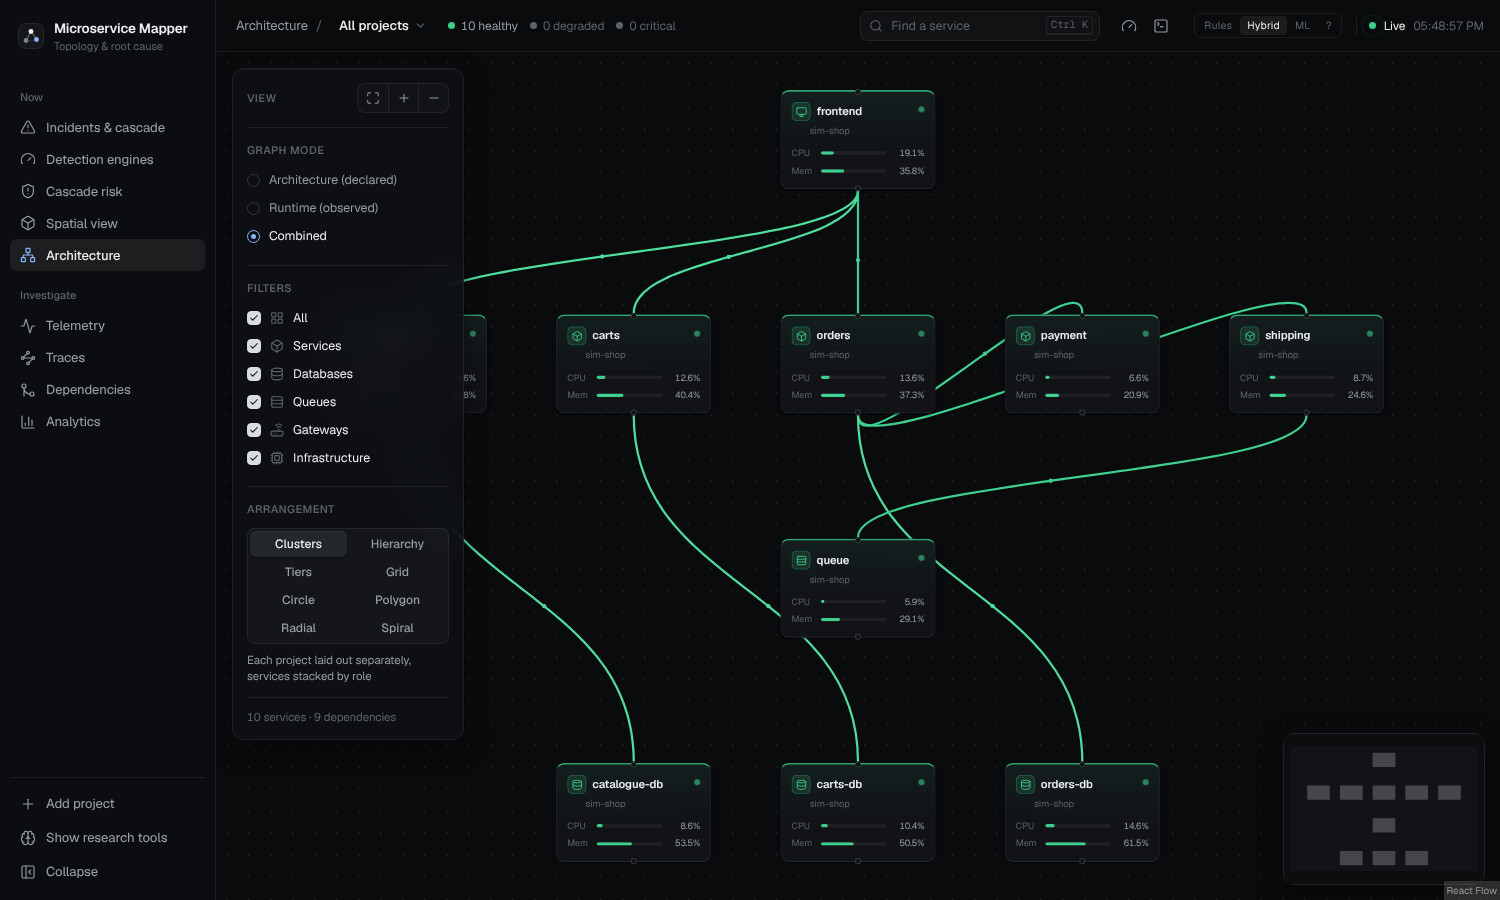
\includegraphics[width=\textwidth]{ui_architecture.jpg}
\caption{Architecture view: the dependency graph of the simulated shop, with arrangement and filter controls.}
\label{fig:ui-arch}
\end{figure}

\subsection{Incidents and cascade}
When the alarm is raised the page shows the most likely root cause, the confidence, the severity and the number of affected services. Below it, the cascade panel shows the source, the services already affected (observed) and those next in line (predicted); the ranking lists each service with the strongest signal behind its score; the ``Why'' panel splits a score into its own-level, symptom-level and walk components and lists the evidence that raised it; and the next steps give concrete commands for the host.

\begin{figure}[!htbp]
\centering
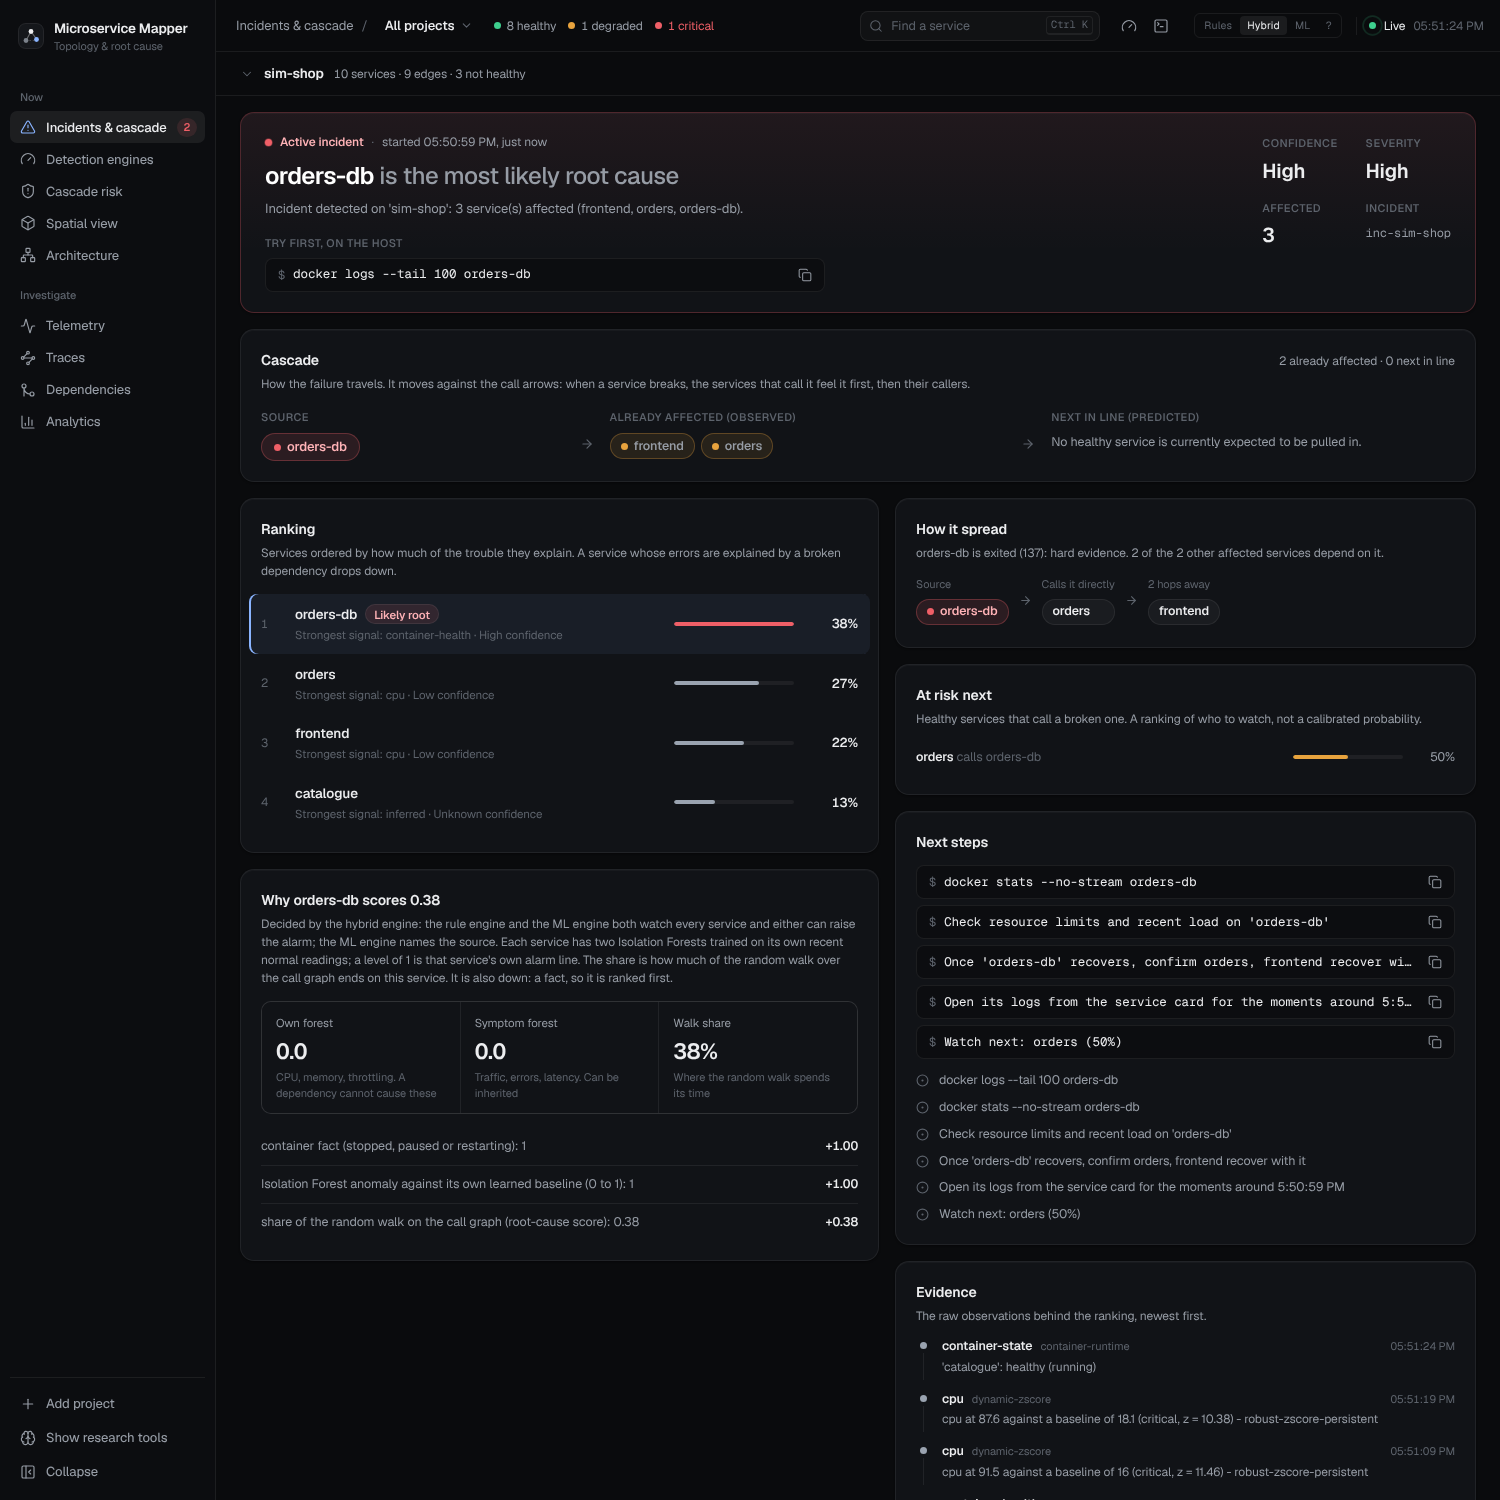
\includegraphics[width=\textwidth]{ui_incident_active.png}
\caption{An active incident after \texttt{orders-db} was killed: root cause, cascade, ranking, evidence breakdown and next steps.}
\label{fig:ui-incident}
\end{figure}

\subsection{Detection engines}
The Detection engines page (Figure~\ref{fig:ui-engines-alarm}) is where a developer checks what the engine switch actually changes. The top half explains the three engines in four short lines each (what decides, how the source is named, the strength, the weakness) and states the Hybrid rule as a formula. Below it the three engines run side by side on the same readings, every cycle, whichever one is active. Each column names its top suspect, and the ML column also says \emph{why}: in Figure~\ref{fig:ui-engines-alarm} it reads ``payment, cpu 10.3 spreads from what the load predicts''. A small chip next to the project name says whether the shared workload moved (``workload steady'' or ``traffic $\times$2.4, explained, not a fault''), so a user can see at a glance that a traffic swing was taken out before any service was judged.

Under the columns are six charts: each engine's peak against its alarm line, a strip showing on which cycles the engines agreed, the level of every service under every engine, a source-or-victim scatter (own resources against symptoms), the share of blame from the random walk, and a trail for one chosen service. Every chart has an enlarge button; the enlarged view (Figure~\ref{fig:ui-engines-popup}) adds a time brush so a stretch of a few cycles can be zoomed into, and closes with Esc. The page ends with the configuration of both engines in plain words.

\begin{figure}[p]
\centering
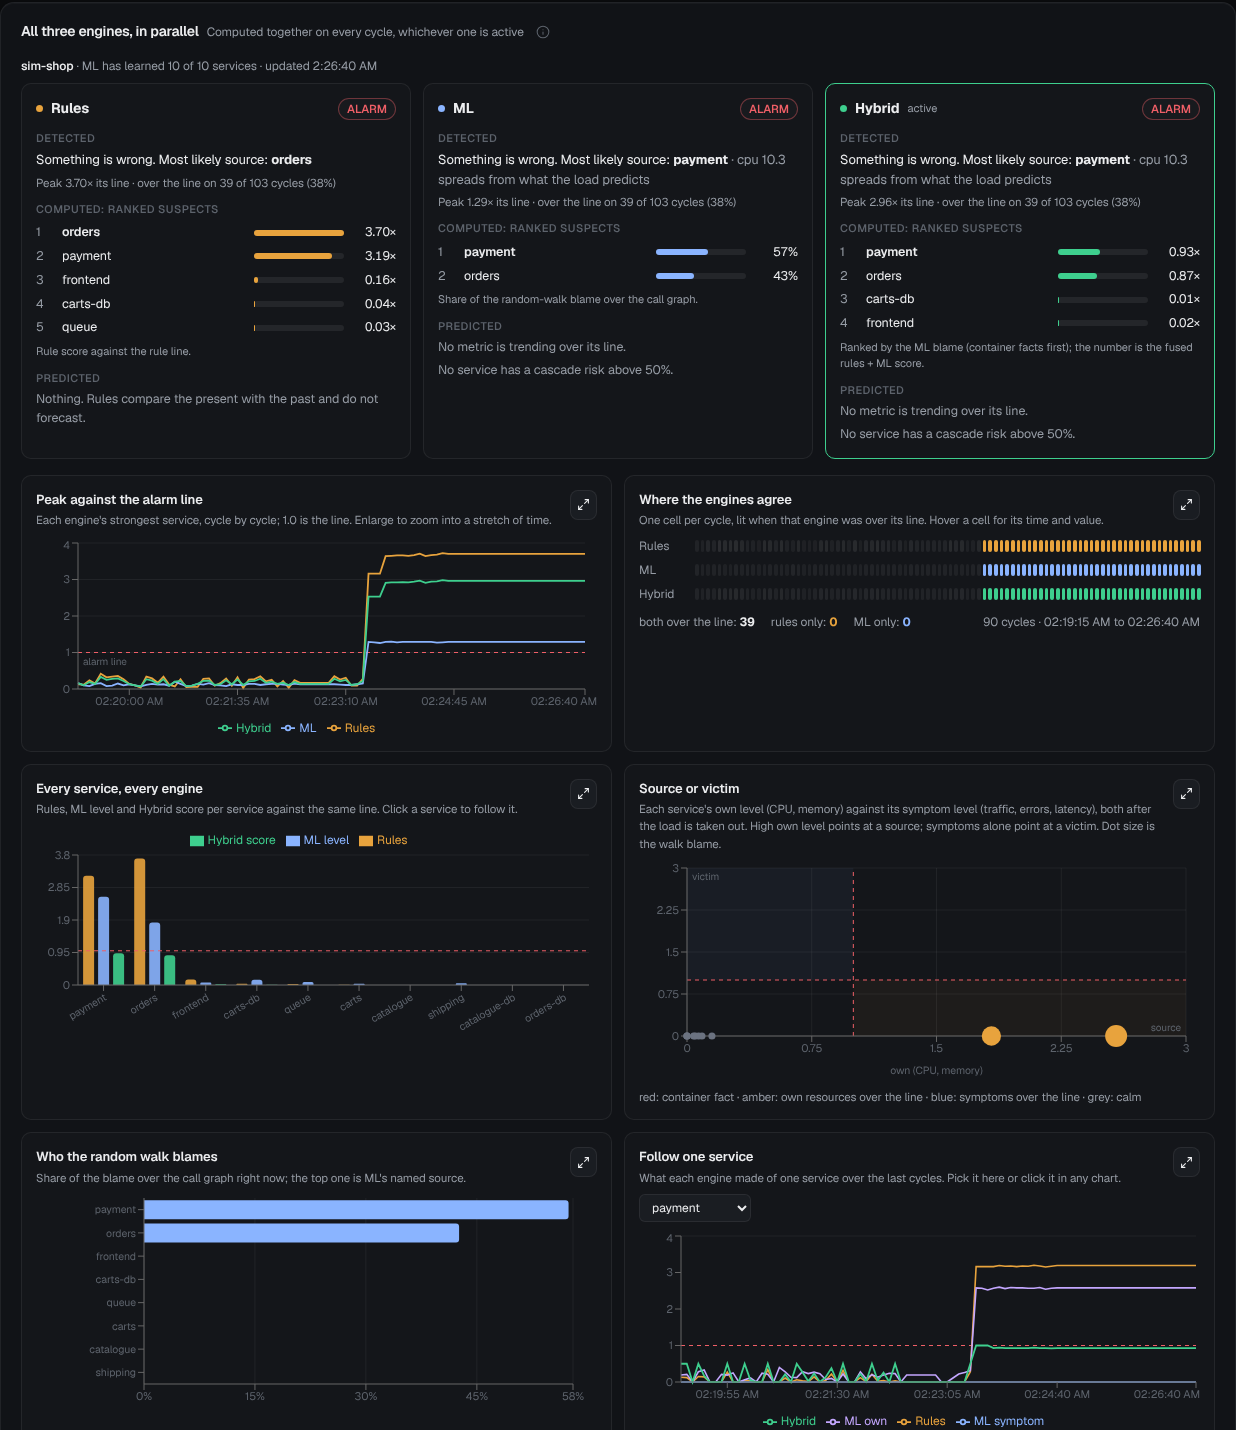
\includegraphics[width=0.96\textwidth,height=0.82\textheight,keepaspectratio]{ui_engines_alarm.png}
\caption[The Detection engines page during a slow-payment fault]{The parallel view during a slow-payment fault. Rules blame \texttt{orders} (the louder victim); ML and Hybrid name \texttt{payment} and say which signal moved. Below: peak against the line, agreement strip, every service, source or victim, walk blame and one service's trail.}
\label{fig:ui-engines-alarm}
\end{figure}

\begin{figure}[!htbp]
\centering
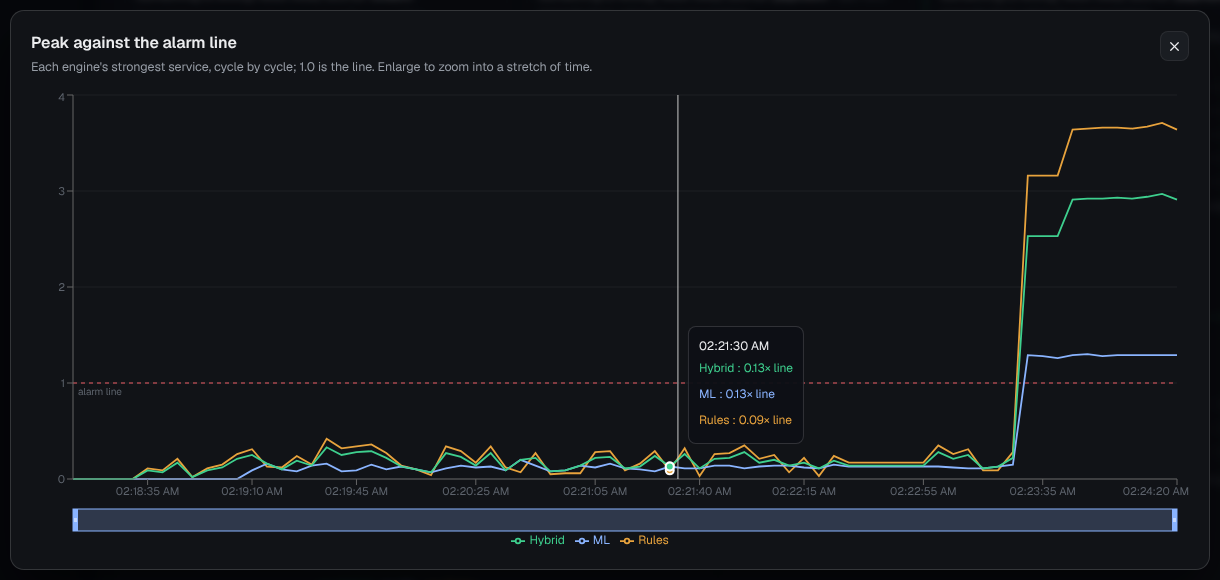
\includegraphics[width=0.82\textwidth]{ui_engines_popup.png}
\caption[An enlarged engine chart with its time brush]{An enlarged chart with its time brush and hover read-out. The ML peak crosses the line once and stays just above it; the rule score climbs higher but on the wrong service.}
\label{fig:ui-engines-popup}
\end{figure}

\subsection{Cascade risk}
The cascade-risk page shows what is failing now and on its own measurements, what is exposed, and what would happen if a chosen service failed (what-if), with the model's name and parameter beside every prediction rather than a bare number.

\begin{figure}[!htbp]
\centering
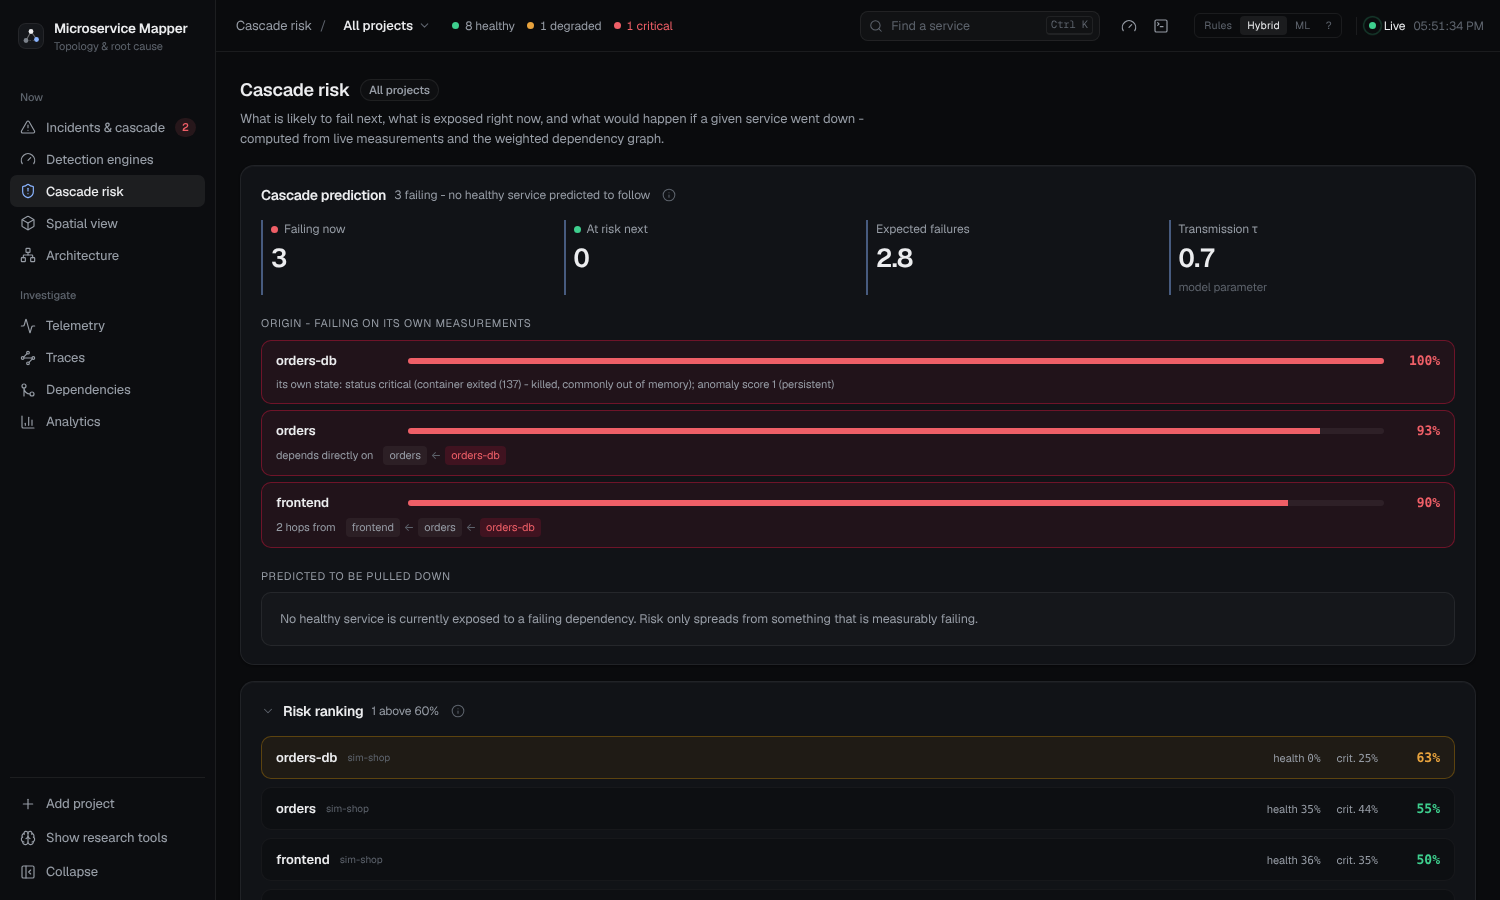
\includegraphics[width=\textwidth]{ui_cascade_risk_fault.png}
\caption{Cascade risk during the fault: the origin and the services failing on their own measurements, expected failures and transmission.}
\label{fig:ui-cascade}
\end{figure}

\subsection{Telemetry, traces, dependencies and analytics}
Four pages support the investigation (Figure~\ref{fig:ui-pages}). Telemetry shows fleet totals, the live connection log and a sortable per-service table with a history chart. Traces shows connection tracing as a ring, a matrix and an event stream; these are sampled TCP sockets, not requests. Dependencies lists every connection with its declared and observed flags and its evidence sources. Analytics gives a health index, the counts of healthy, degraded and critical services, the most connected services and the top CPU and memory users.

\begin{figure}[!htbp]
\centering
\setlength{\tabcolsep}{2pt}
\begin{tabular}{cc}
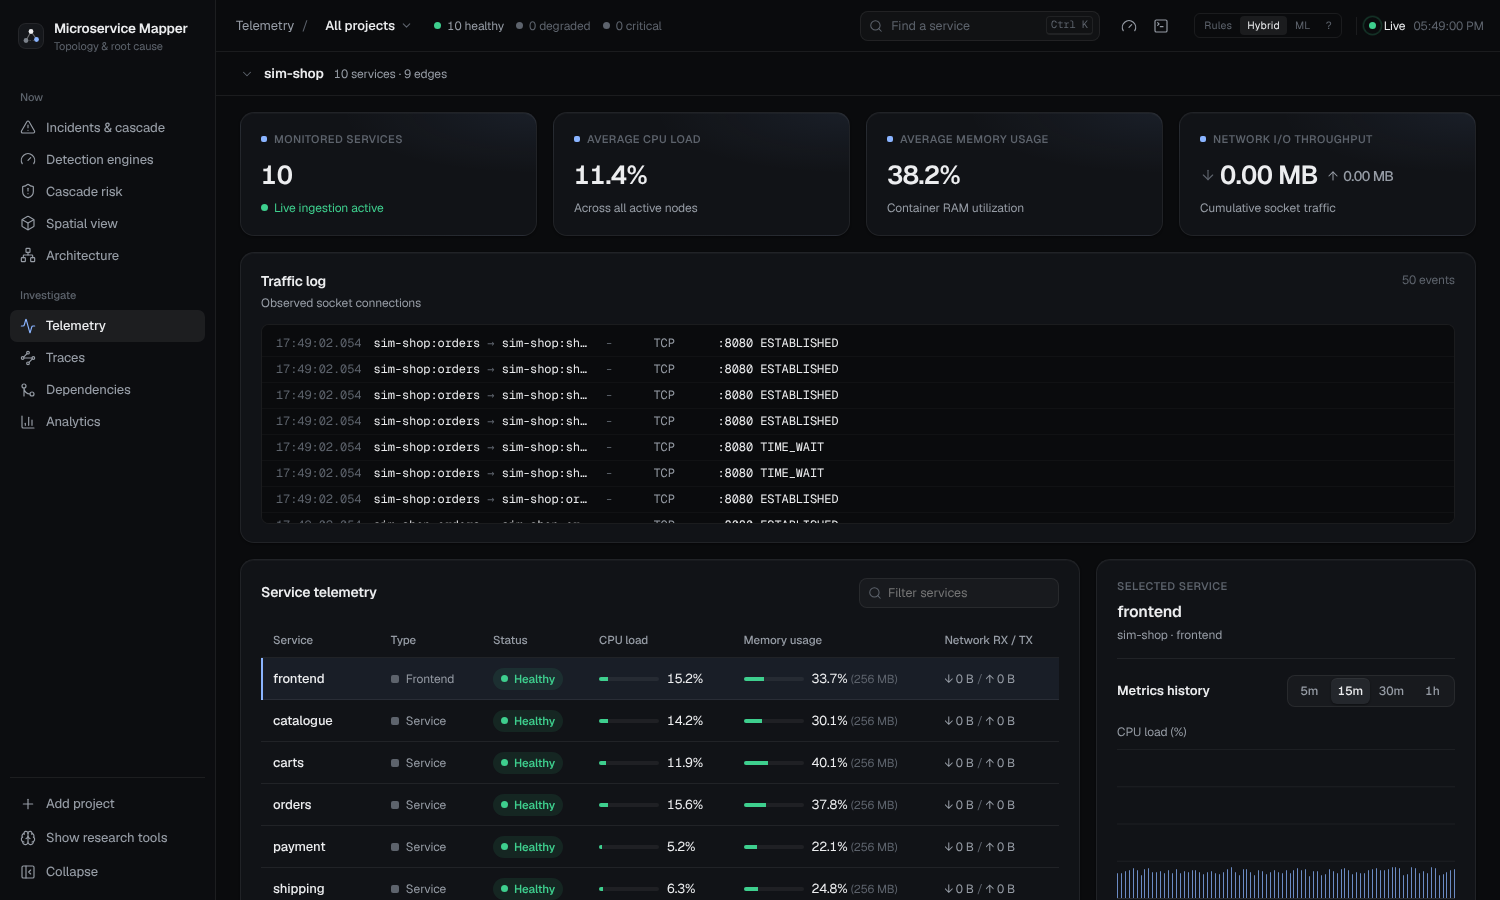
\includegraphics[width=0.49\textwidth]{ui_telemetry.png} & 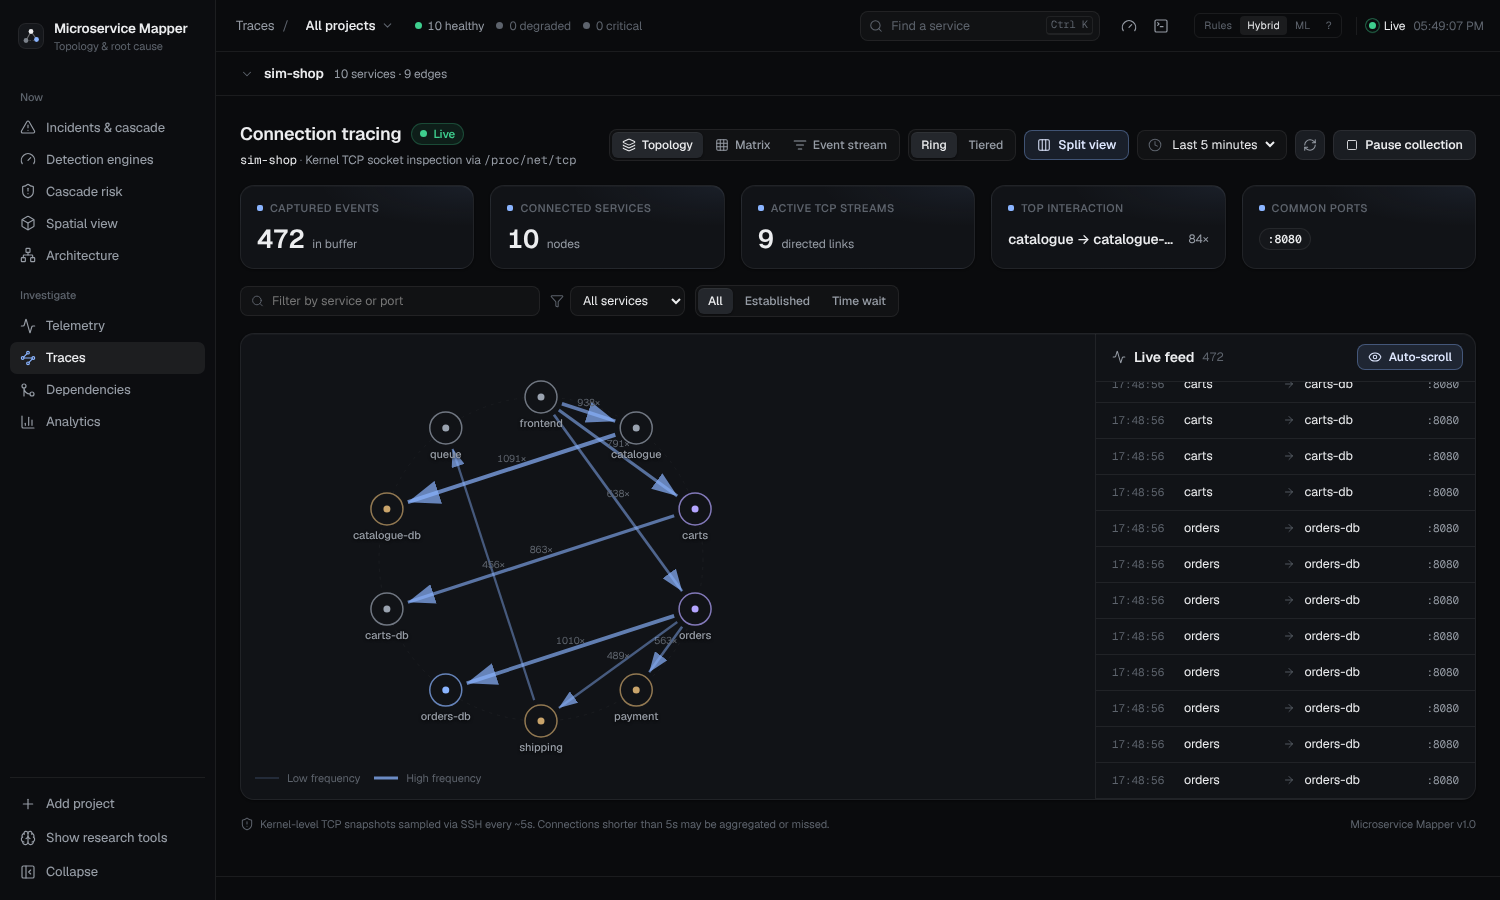
\includegraphics[width=0.49\textwidth]{ui_traces.png}\\
\small (a) Telemetry & \small (b) Traces\\[4pt]
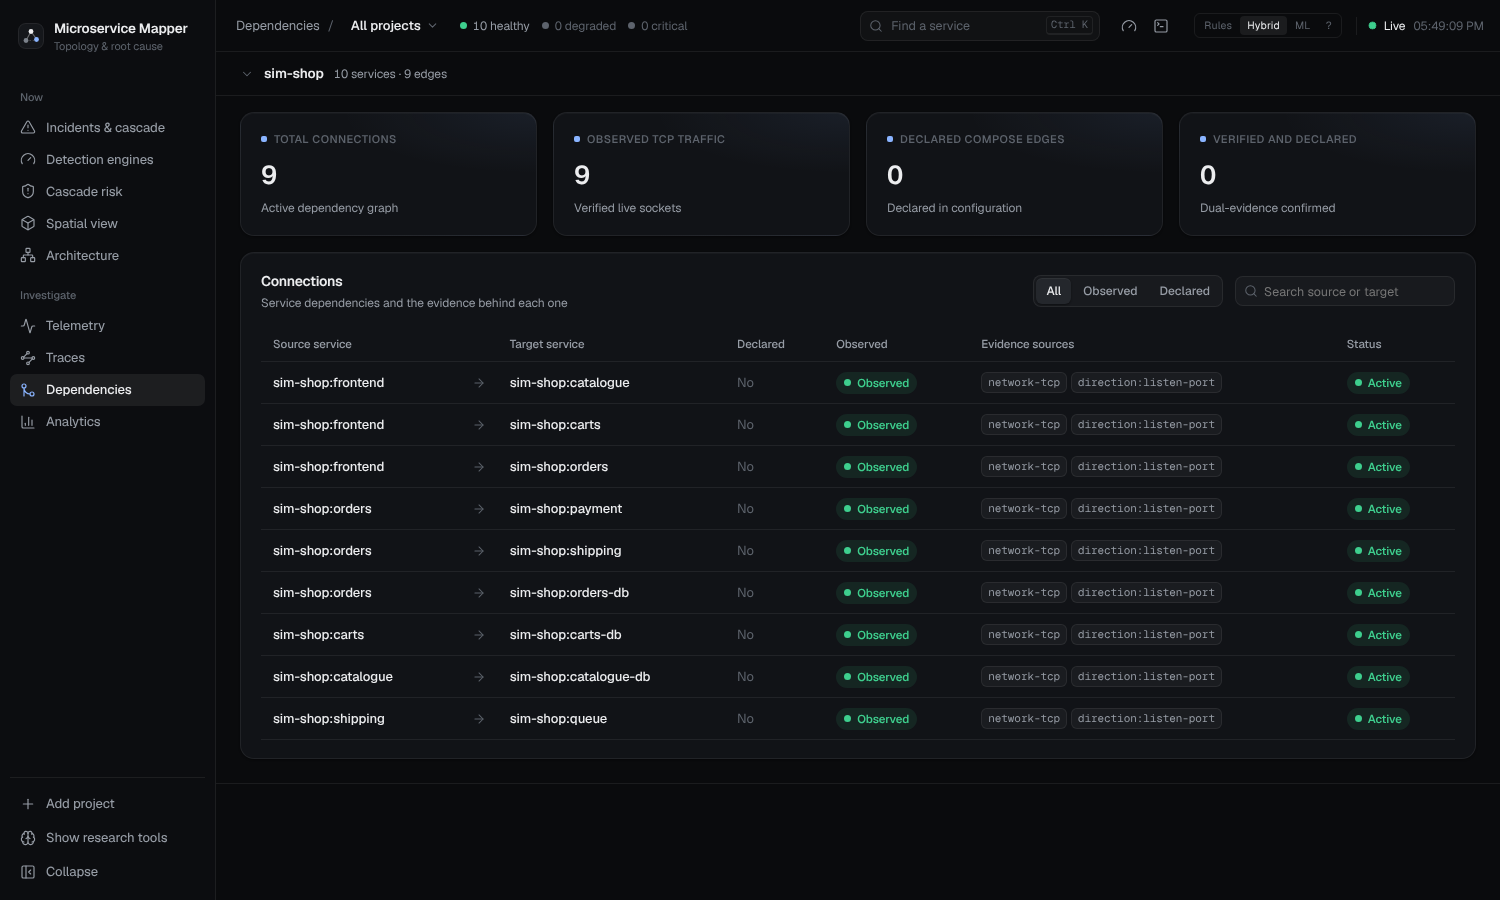
\includegraphics[width=0.49\textwidth]{ui_dependencies.png} & 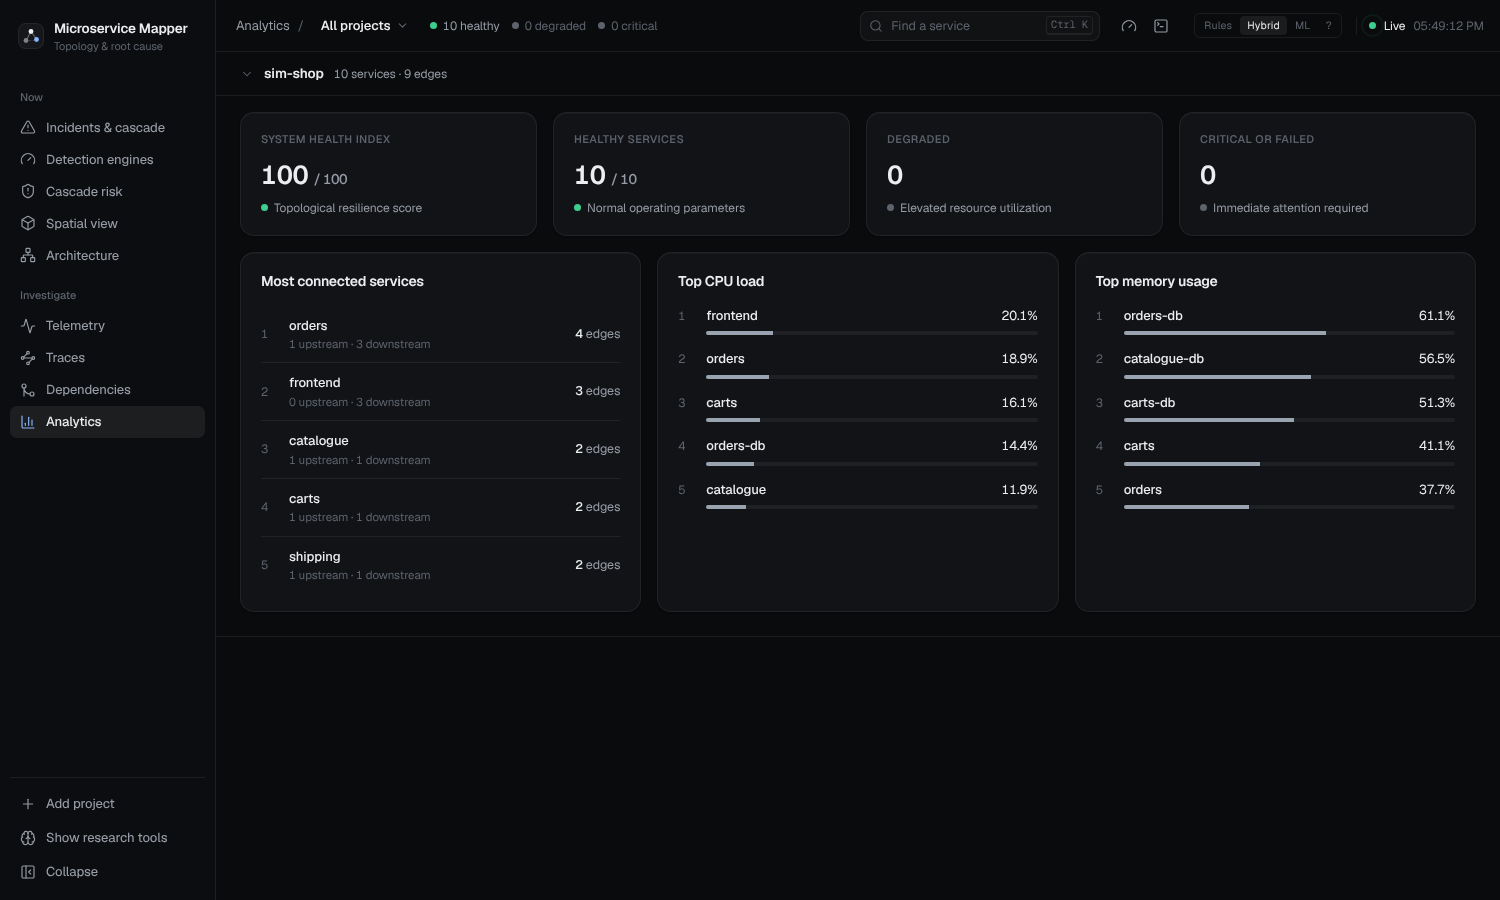
\includegraphics[width=0.49\textwidth]{ui_analytics.png}\\
\small (c) Dependencies & \small (d) Analytics
\end{tabular}
\caption[The telemetry, traces, dependencies and analytics pages]{The investigation pages: (a) telemetry with fleet totals and a per-service table, (b) connection traces as ring, matrix and event stream, (c) dependencies with their evidence (here \emph{network-tcp} and \emph{direction:listen-port}), (d) analytics.}
\label{fig:ui-pages}
\end{figure}

\subsection{The 3D spatial view}
The 3D scene shows the same graph as a small city, and each arrangement answers a different question a developer asks while debugging. Services are units on platforms; links are cables whose thickness shows the dependency weight and whose colour shows the heat of the link, with pulses that move at a rate driven by the link's request rate. A floating card over each platform gives its role, how many services it holds and their state. The figures were taken on the live ShopFlow bench, with the scene focused on that project.
\begin{itemize}
\item \textbf{Islands} (Figure~\ref{fig:3d-islands}) groups services by role: edge, services, messaging and data, each on its own raised platform.
\item \textbf{Flow} (Figure~\ref{fig:3d-views}a) lays the platforms out in the order a request travels: the entry points, then the services one hop away, two hops away and so on. Each card says how many callers a fault at that hop can reach, so the platform to look at first is the one whose card says the most.
\item \textbf{Topology} (Figure~\ref{fig:3d-views}b) sorts services by how much depends on them: the most depended-on, the depended-on, and those nothing depends on. It is the blast-radius view: a fault on the first platform hurts the most.
\item \textbf{Tiers} (Figure~\ref{fig:3d-views}c) stacks the architectural layers as terraces from edge (L4) down to data (L1), with the calls in and out of each layer on its card, so a call that skips a layer or goes up the stack stands out.
\end{itemize}
During a fault the failing unit is boxed in red with a callout naming it and its score, its platform is tinted, the card changes from ``all healthy'' to the count of degraded services, and the bell in the corner counts what needs attention (Figure~\ref{fig:3d-islands}b).

\begin{figure}[!htbp]
\centering
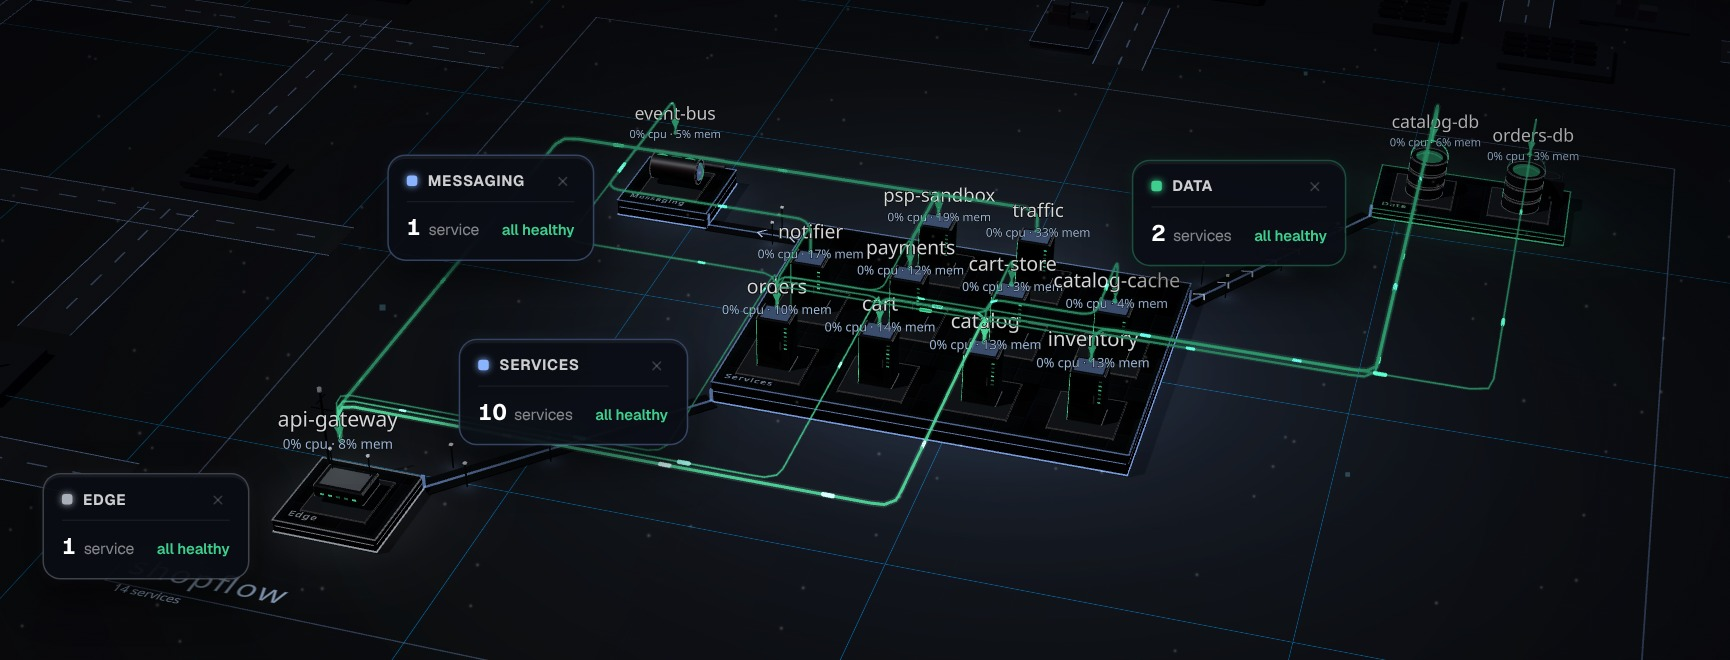
\includegraphics[width=\textwidth]{ui3d_islands.jpg}\\[-1pt]
{\small (a) Healthy}\\[6pt]
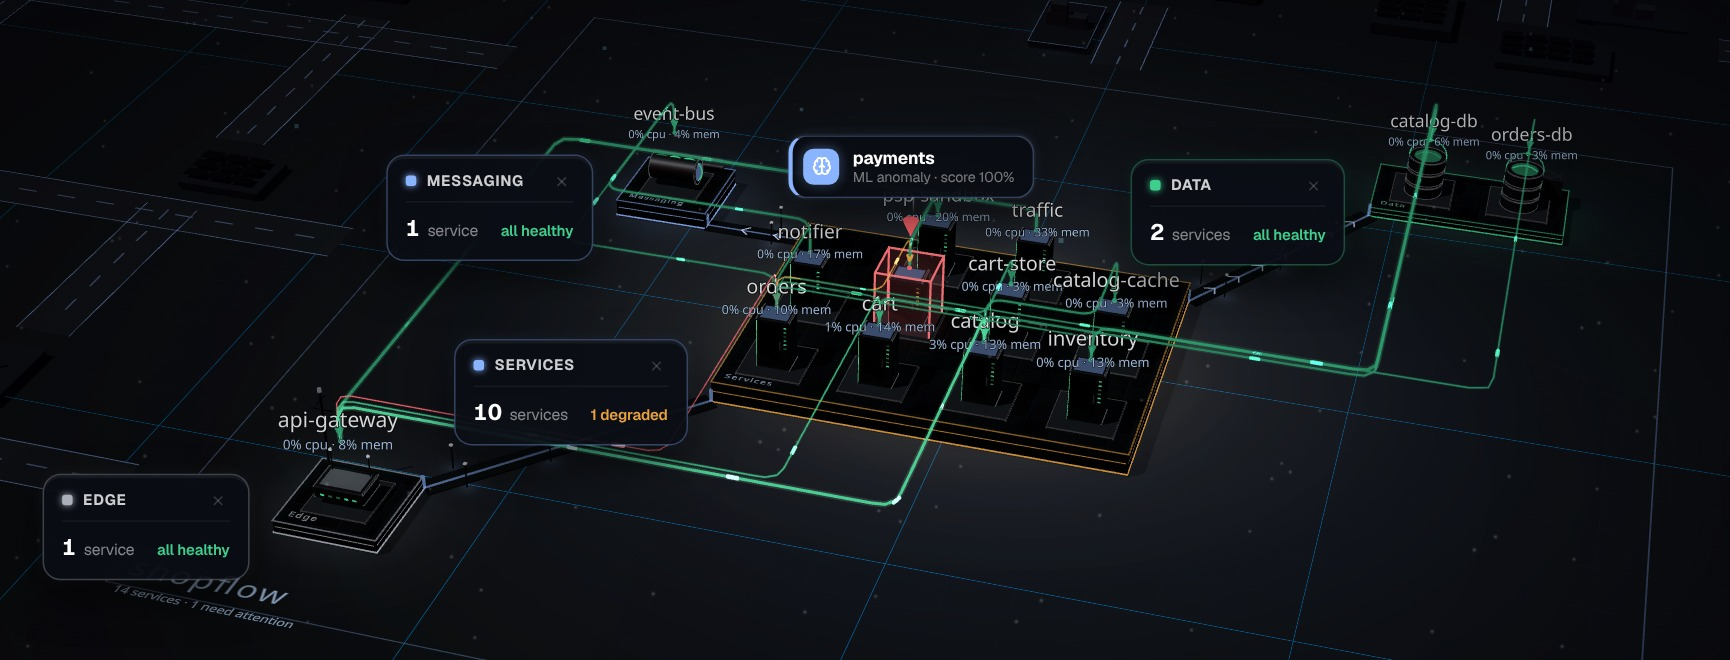
\includegraphics[width=\textwidth]{ui3d_islands_fault.jpg}\\[-1pt]
{\small (b) During a fault: \texttt{payments} paused}
\caption[The 3D Islands view of the ShopFlow bench, healthy and during a fault]{The 3D Islands view of the live ShopFlow bench: one platform per role with a card giving its size and state. (b) The same view with \texttt{payments} paused: the unit is boxed in red, its platform tinted and its card updated.}
\label{fig:3d-islands}
\end{figure}

\begin{figure}[p]
\centering
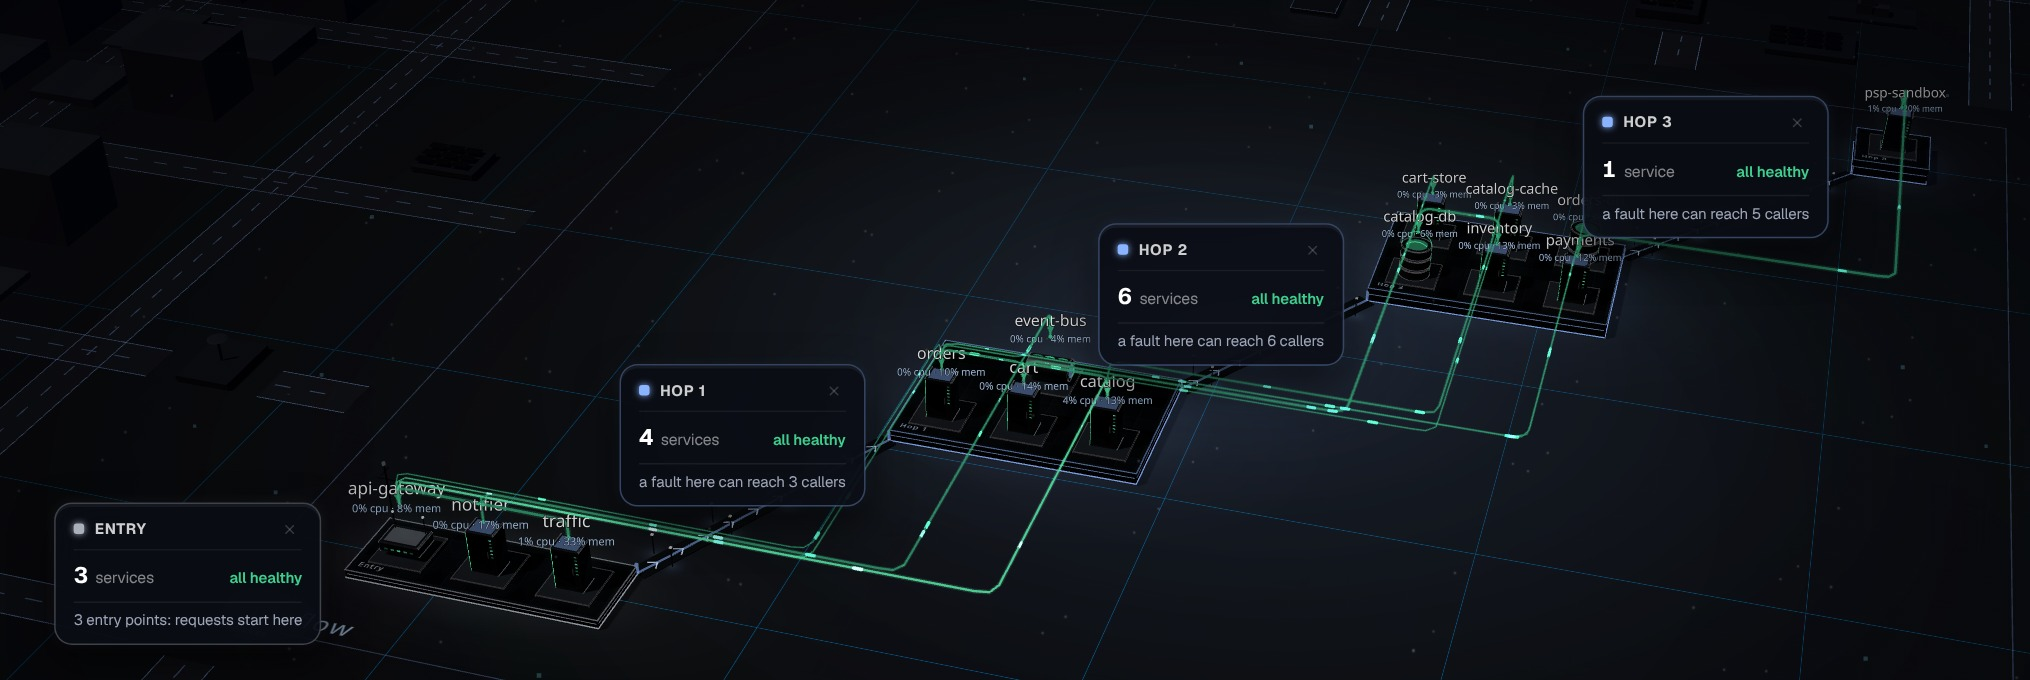
\includegraphics[width=\textwidth]{ui3d_flow.jpg}\\[-1pt]
{\small (a) Flow: the request path, hop by hop}\\[6pt]
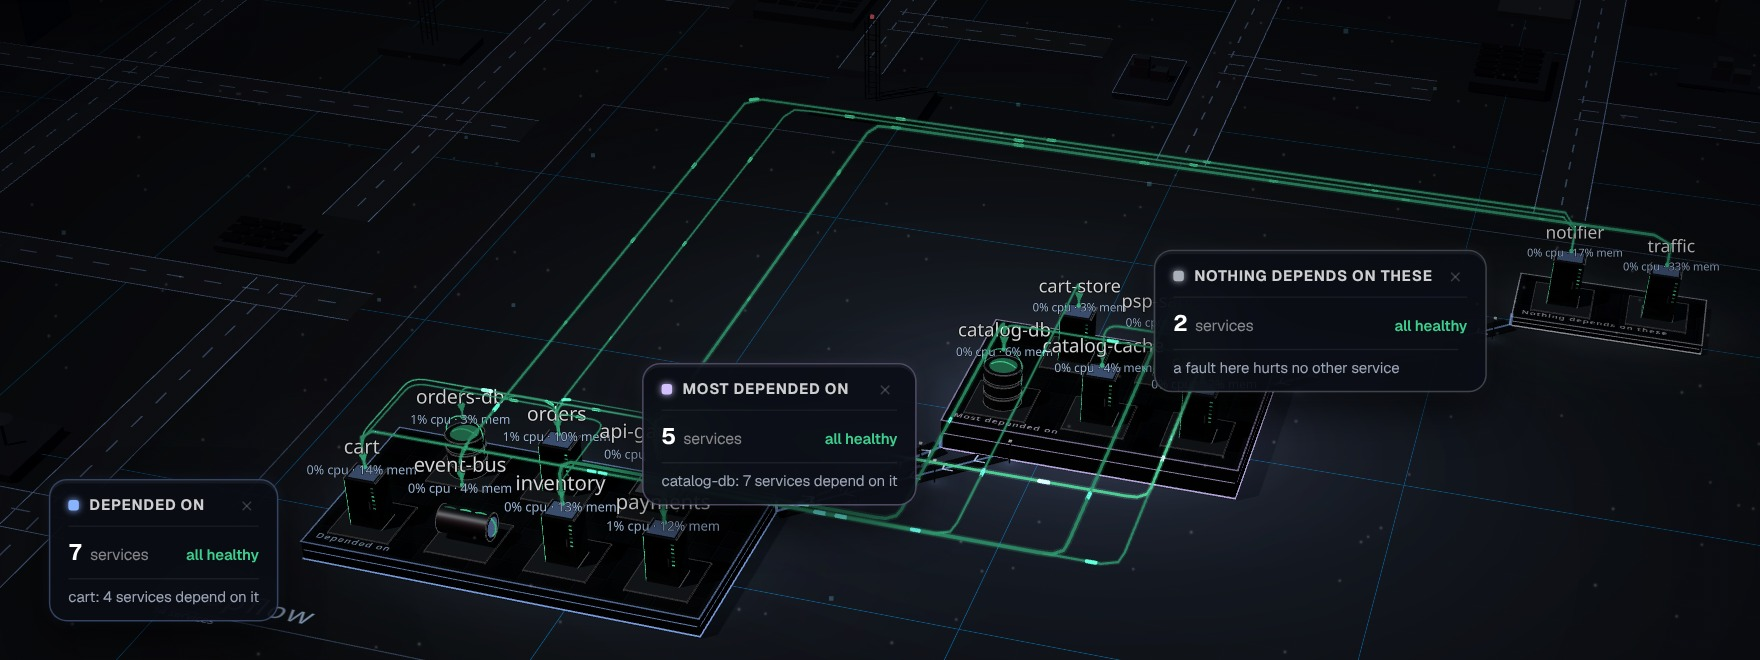
\includegraphics[width=\textwidth]{ui3d_topology.jpg}\\[-1pt]
{\small (b) Topology: by how much depends on each service}\\[6pt]
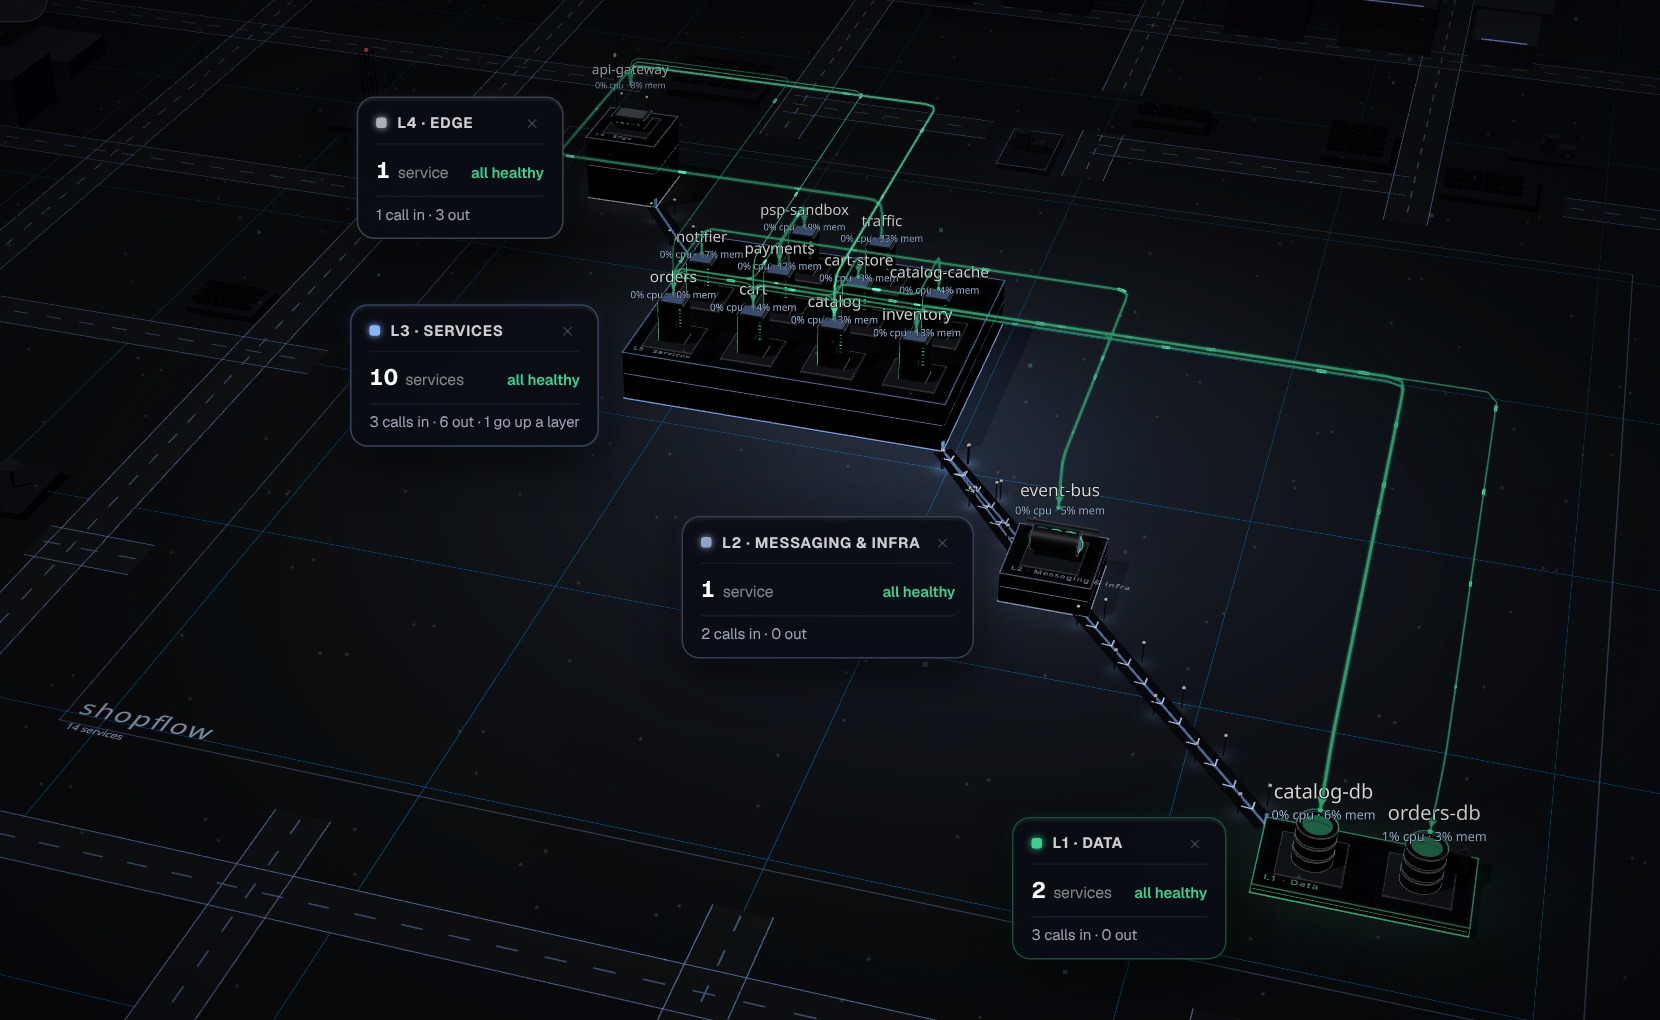
\includegraphics[width=\textwidth]{ui3d_tiers.jpg}\\[-1pt]
{\small (c) Tiers: architectural layers as terraces}
\caption[The Flow, Topology and Tiers arrangements of the 3D view]{The Flow, Topology and Tiers arrangements of the same bench. Each card states what a fault there would mean: how many callers it can reach (Flow), how many services depend on it (Topology), and the calls in and out of each layer (Tiers).}
\label{fig:3d-views}
\end{figure}

\subsection{Research pages}
Three pages that belong to the study rather than daily operation are hidden until the operator switches them on: the ML pipeline (what the hybrid engine sees per service), the model findings of the optional Python sidecar, and the experiment history.

\section{Security Considerations}
\label{sec:security}
The tool holds SSH access to hosts, so it was built to expose as little as it can.
\begin{itemize}
\item \textbf{Keys stay on the operator's machine.} The configuration stores only the path of the key file. Private keys are never copied into the repository, and \texttt{*.pem} files are git-ignored as a backstop.
\item \textbf{A fixed command catalogue.} Every command the server can run on a host is built by a function in one file, and every argument that reaches a shell is checked against the shapes Docker itself produces (container identifiers, timestamps, tail lengths, paths). A test checks that an identifier with shell metacharacters is refused before a command is built.
\item \textbf{Bounded output and time.} Each command has a timeout and a maximum output size, so a misbehaving host cannot make the server wait or buffer without limit.
\item \textbf{Local control surfaces.} The Fault Lab panel listens on localhost only and its requests need a header the page itself sets. Grafana and Prometheus listen on localhost and are reached through an SSH tunnel.
\item \textbf{Ingest token.} The push endpoint is protected by a token. The built-in default is for local use and must be changed when the server can be reached by others.
\item \textbf{One write on the host.} The only change the mapper makes on a host is restarting a container that exited with a non-zero code, a few attempts at most per container, never for load generators, and switched off with \texttt{MAPPER\_AUTO\_RESTART=off}.
\item \textbf{Load limits.} The traffic generator clamps the number of virtual users to a fixed ceiling and starts only from the traffic controller.
\end{itemize}

\section{Testing and Validation}
\label{sec:testing}
The suite has 339 tests in 19 suites and runs in under a minute with \texttt{npm test}. Table~\ref{tab:tests} groups them by area. Three kinds of test deserve a note. \emph{Purity tests} check that algorithm modules do not touch the filesystem or the network, so they can be replayed. \emph{Regression tests} hold each bug that was found (for example the ledger-reader bug and the tier layout). \emph{Security tests} check that the command catalogue refuses unsafe identifiers.

\begin{table}[!htbp]
\centering
\caption{The test suites.}
\label{tab:tests}
\small
\renewcommand{\arraystretch}{1.2}
\begin{tabularx}{\textwidth}{>{\raggedright\arraybackslash}p{5.3cm}>{\raggedright\arraybackslash}X}
\toprule
\textbf{Suite(s)} & \textbf{What is held}\\
\midrule
\texttt{logic}, \texttt{riskEngine}, \texttt{rca} & Layouts (2D and 3D), edge heat scale, risk, cascade, what-if, root-cause scoring\\
\texttt{ml-engine}, \texttt{ml}, \texttt{load-model}, \texttt{rca-research} & Load-aware model (workload invariance, a fault seen during a load change), walk, propagation, hybrid fusion, learned directions, change points\\
\texttt{pipeline}, \texttt{eval}, \texttt{purity} & End-to-end replay, scoring against a ledger, purity of algorithm modules\\
\texttt{telemetry-platform.*} (eight files) & SSH connection, command catalogue, Docker parsers, CPU, units, service identity, storage, discovery, metric collector\\
\texttt{sockets}, \texttt{requestStats}, \texttt{freshness} & Socket direction and recently closed sockets, request statistics, staleness\\
\texttt{security}, \texttt{platform} & Command sanitising, portability across operating systems\\
\texttt{edge-cases}, \texttt{sparse-traffic}, \texttt{target-model} & Missing data, idle services, per-target models\\
\bottomrule
\end{tabularx}
\end{table}

\section{The Two Custom Benchmark Hosts: ShopFlow and LedgerLine}
\label{sec:benches}
The two real systems of the evaluation are not borrowed demos. They were built for this study as \emph{test benches for root-cause-analysis tooling}, each in its own repository and each running on its own EC2 host. The code of both is correct and defensive: every failure comes from configuration, data volume, sizing, topology or a third party, and every failure ships with a machine-readable ground truth (the true root cause, what a monitor should and should not be able to see, and the fix). Each bench has the same four parts: the application, a monitoring stack with Grafana, an always-on traffic generator, and a Fault Lab.

\begin{table}[!htbp]
\centering
\caption{The two benchmark hosts.}
\label{tab:benches}
\small
\renewcommand{\arraystretch}{1.2}
\begin{tabularx}{\textwidth}{>{\raggedright\arraybackslash}p{3.2cm}>{\raggedright\arraybackslash}X>{\raggedright\arraybackslash}X}
\toprule
 & \textbf{ShopFlow} & \textbf{LedgerLine}\\
\midrule
Domain & Online retail checkout & Retail-banking transfers\\
Services & Gateway, catalogue, cart, inventory, payments, orders, an order-event consumer, a third-party payment sandbox; two PostgreSQL, two Redis, NATS (13 services) & Edge, accounts, transfers, fraud screening, FX rates, a double-entry ledger, a statements worker, a third-party FX provider; two PostgreSQL, Redis, NATS (12 services)\\
Public port & 8080 (storefront and API) & 8081 (gateway)\\
Host & EC2 \texttt{c7i-flex.large}, Ubuntu 24.04; about 0.6\,GiB of containers & the same\\
Scenarios with ground truth & 12 (one baseline control) & 7 (one baseline control)\\
Monitoring & Prometheus, Grafana, Loki, Promtail; 25-panel dashboard & the same stack; 25-panel dashboard\\
\bottomrule
\end{tabularx}
\end{table}

\subsection{Monitoring, traffic and the Fault Lab}
Each bench carries a monitoring stack as a \emph{separate Compose project}, so the application project stays exactly what a mapper should discover: Prometheus, Grafana with a provisioned 25-panel dashboard (Figure~\ref{fig:grafana-sf}), Loki with Promtail, and a small exporter that reads per-container CPU, memory, network, restarts and health from the Docker API. Grafana is the operator's ordinary view of a healthy and a faulted bench, and an independent source against which the mapper's readings can be compared on the same time axis. Everything listens on localhost and is reached through an SSH tunnel.

Each bench also has an always-on, open-loop traffic generator. The default mode is \emph{organic}: visitor sessions with think times, popular products, returning users and a day-and-night wave; a steady mode gives a flat load and a quiet mode stops it.

The Fault Lab (\texttt{lab/faultlab} in each bench repository, Figure~\ref{fig:faultlab-sf}) is the fault injector of the evaluation. It is \textbf{blind}: the mapper is never told what is injected, and everything is written to a private ledger read only when scoring. It is \textbf{physical}: faults act on containers (kill, repeated kills, stop, pause, resource limits, network detach, pause-and-release cycles). It is \textbf{organic and reproducible}: a campaign draws faults from a Poisson process with a profile, rate and seed, and the same seed gives the same campaign. Its control page runs on the bench host, listens on localhost only and needs a header the page itself sets, so another site open in the same browser cannot drive it.

\begin{figure}[!htbp]
\centering
\begin{minipage}[b]{0.40\textwidth}\centering
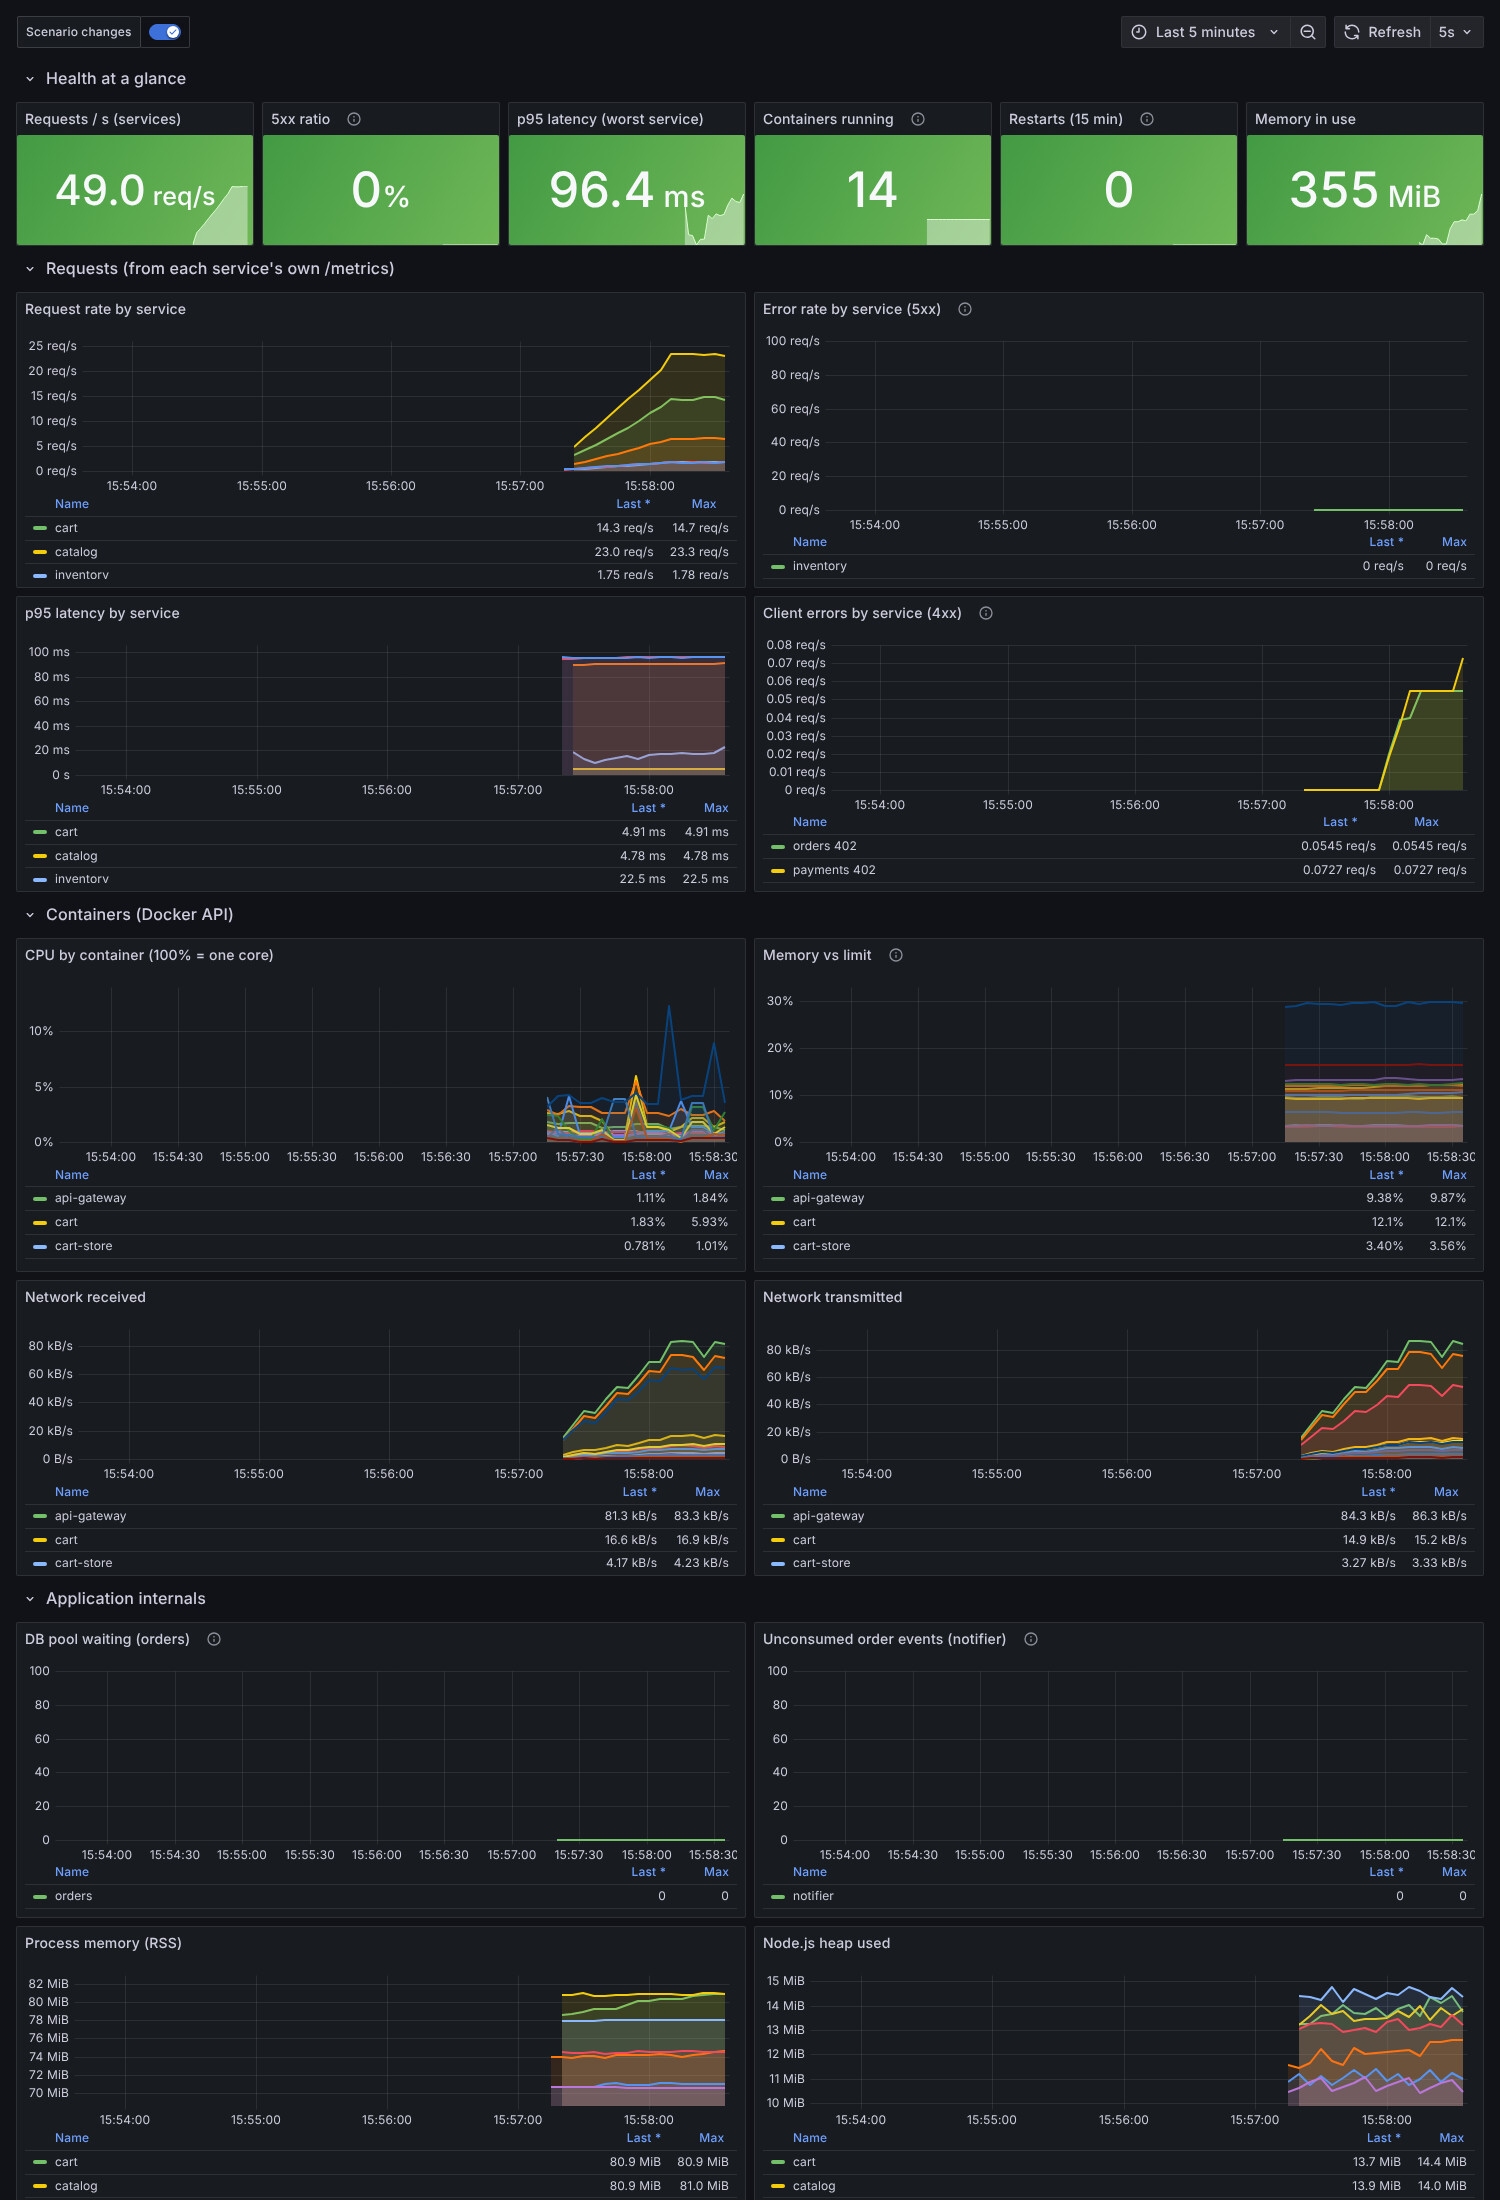
\includegraphics[width=\linewidth]{grafana_shopflow.jpg}
\caption[The provisioned Grafana dashboard of the ShopFlow bench]{The provisioned Grafana dashboard of the ShopFlow bench, from the running bench.}
\label{fig:grafana-sf}
\end{minipage}\hfill
\begin{minipage}[b]{0.56\textwidth}\centering
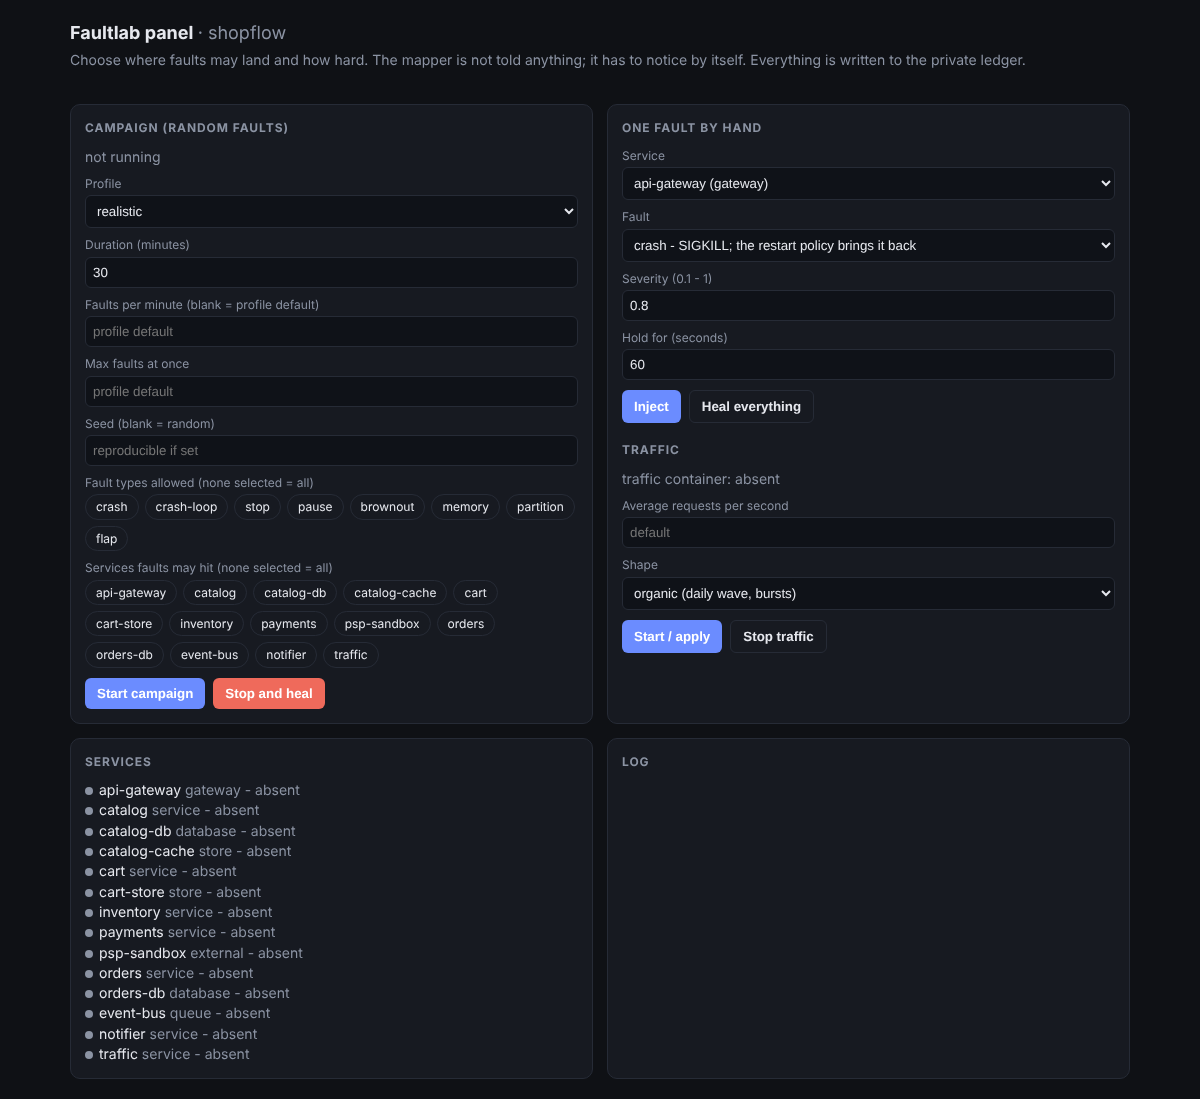
\includegraphics[width=\linewidth]{faultlab_shopflow.png}
\caption[The Fault Lab control page of the ShopFlow bench]{The Fault Lab control page of the ShopFlow bench: a random campaign, one fault by hand, traffic control and the service list.}
\label{fig:faultlab-sf}
\end{minipage}
\end{figure}

\subsection{Scenarios with ground truth}
Besides random campaigns, each bench offers scripted scenarios. A scenario applies a defined cause, drives the load that triggers it, and writes a report beside the expected result stated in its \texttt{scenario.yaml}. Table~\ref{tab:scen-sf} lists those of ShopFlow; LedgerLine has seven more (a pool-starvation cycle between two healthy services, a third-party outage behind a circuit breaker, a hot row, a connection budget, a month-end job that runs out of memory, a shadow dependency, and a baseline). They cover cascades, retry amplification, silent degradation and undocumented dependencies, which are the cases a diagnosis tool most easily gets wrong. The random campaigns of Chapter~\ref{ch:method} are what the reported numbers come from.

\begin{table}[!htbp]
\centering
\caption{ShopFlow scenarios and their true root causes.}
\label{tab:scen-sf}
\footnotesize
\renewcommand{\arraystretch}{1.15}
\begin{tabularx}{\textwidth}{>{\raggedright\arraybackslash}p{3.3cm}>{\raggedright\arraybackslash}X>{\raggedright\arraybackslash}p{2.4cm}}
\toprule
\textbf{Scenario} & \textbf{What happens} & \textbf{Root cause}\\
\midrule
sf-01-missing-index & Order history is fast in staging, melts the database in production & orders-db\\
sf-02-cache-thrash & A cache sized for staging evicts itself in production & catalog-cache\\
sf-03-unbounded-cache & Memory climbs for an hour, then the container is killed & cart\\
sf-04-retry-storm & A third party throttles; our own retries make it ten times worse & psp-sandbox\\
sf-05-secret-rotation & A rotated database password; one service still has the old one & orders\\
sf-06/07 & A dependency that exists only in the code; a declared one nobody calls & none\\
sf-08-noisy-neighbor & A reporting job on the shared database slows checkout & catalog-db\\
sf-09-cpu-throttle & Slow but healthy: a container throttled at a quarter of a core & catalog\\
sf-10-poison-message & One un-processable message stops every confirmation e-mail & notifier\\
sf-11-wrong-hostname & A renamed service still referenced by its old name & none\\
\bottomrule
\end{tabularx}
\end{table}

\section{Host and Mapper Diagnostic Tools}
\label{sec:tools}
Operating the benches showed that ``nothing appears in the dashboard'' has two very different causes: the host cannot answer, or the mapper has a problem. \textbf{\texttt{npm run check-host}} walks one instance step by step and stops at the first failure (port 22, key permissions, login, memory and disk, whether \code{docker} answers within 25 seconds, whether the application answers, which peers each front end calls). \textbf{\texttt{npm run mapper-edges}} prints what the running mapper holds for a project: the target's status, its nodes and every edge with its evidence and last-seen time. Together they separate a host problem from a mapper problem in minutes.

\section{The Evaluation Harness}
\begin{table}[!htbp]
\centering
\caption{The evaluation harness and the experiments built on it.}
\label{tab:harness}
\small
\renewcommand{\arraystretch}{1.2}
\begin{tabularx}{\textwidth}{>{\raggedright\arraybackslash}p{4.4cm}>{\raggedright\arraybackslash}X}
\toprule
\textbf{Command or folder} & \textbf{Purpose}\\
\midrule
\texttt{npm run eval} & Record a fault-injection campaign and score the live mapper (observe, score, report)\\
\texttt{npm run ml:compare} & Compare detectors and root-cause methods on the recorded runs\\
\texttt{npm run ml:hybrid} & Fusion variants of rules and ML\\
\texttt{npm run ml:predict} & Early warning and cascade prediction\\
\texttt{npm run ml:synth} & Synthetic generator (amplification factor, class filter)\\
\texttt{npm run ml:bench} & Cost of one decision window\\
\texttt{v2/} & Studies: learned directions, change-point onset, fault diagnosis\\
\texttt{paper/exp} & Curves, amplification, cascade, router and scaling data for the figures\\
\texttt{run/recorded-runs} & The two recorded runs\\
\bottomrule
\end{tabularx}
\end{table}

\clearpage
\chapter[RESULTS, ANALYSIS AND DISCUSSION]{Results, Analysis and Discussion}
\label{ch:results}

\section{Results}\label{sec:resultsmain}

\subsection{A change of workload is not a fault: the ML correction}
\label{sec:workloadres}
The first ML engine judged each service with two Isolation Forests fitted on that service's recent readings. On the benchmark faults it looked fine, but an operator who stopped the traffic generator and switched to the ML engine saw every service with an anomaly score of 100\%. We reproduced it on recordings made for the purpose. Both benches ran live in Docker, reached by the mapper over SSH, with \emph{no fault at all}; only the work changed (\code{run/scripts/workload-shift-experiment.sh} and \code{workload-steps-experiment.sh}). In the first pair of recordings (two benches, 62 minutes) the organic traffic generator ran, stopped, ran, stopped longer and ran again. In the second pair (two benches, 72 minutes) a closed-loop generator held a constant number of visitors and stepped it $2 \to 8 \to 2 \to 0 \to 20 \to 2$, which moved the entry service's network traffic between 0 and about $3 \times 10^{5}$\,B/s (Figure~\ref{fig:workload}a). Every alarm in these recordings is a false alarm by construction.

The forest was in alarm for 23\% of the organic recording and for 52\% of the steady-load recording (Figure~\ref{fig:workload}b, Table~\ref{tab:models}). The other workload-blind detectors do the same or worse, from 38\% to 75\% on the organic recording and from 76\% to 96\% on the steady one, because all of them model the readings themselves and a new workload is outside what they were fitted on. It is not a tuning matter. A forest scores a value beyond its training range no higher than its most extreme training point, so the old engine had added a range guard. That guard fires at once for every service when the traffic changes for all of them, and a large shift needed thirty minutes to be accepted as the new normal. On the fault-free stretches of the live fault campaigns the same engine raised 40.9 alarm episodes per hour.

The corrected engine (Section~\ref{sec:load}) does not alarm on either recording (0\% and 0\% of the time; one false episode in 72 minutes of steady-load steps, none in 62 minutes of organic traffic). Figure~\ref{fig:workload}c shows the load factor it read: it follows the steps of Figure~\ref{fig:workload}a. It rises to about $+2$ at the twenty-visitor step (traffic about seven times the reference) and falls to about $-1.2$ when the traffic stops (the log scale saturates at the network unit). That is how the shift gets explained instead of judged. The model finds the change by itself: no setting names the load generator, and nothing is installed on the hosts.

\begin{figure}[!htbp]
\centering
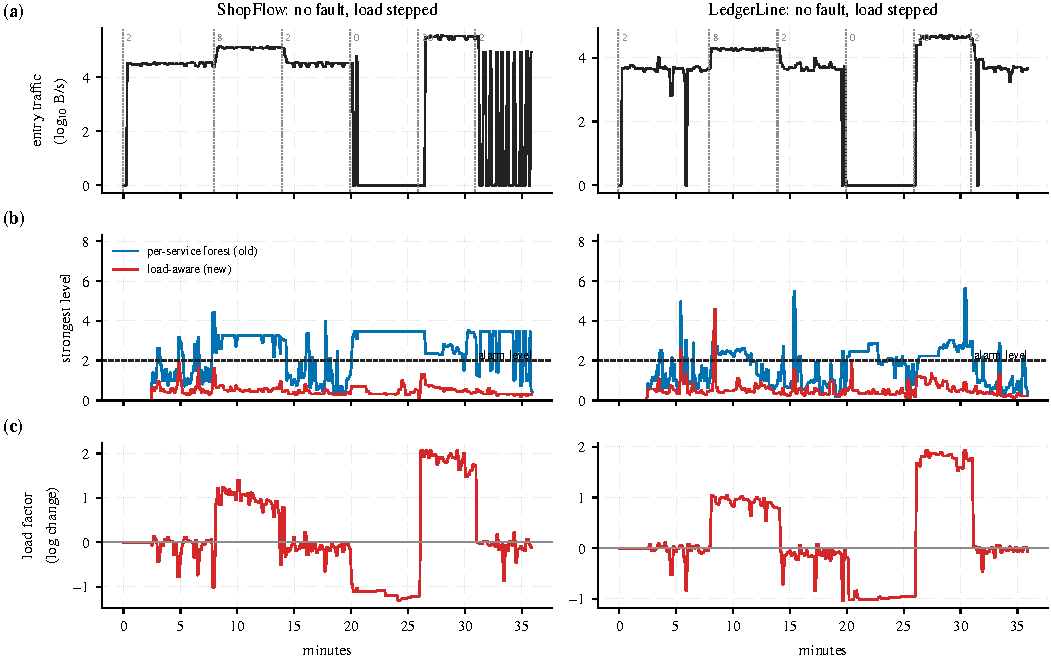
\includegraphics[width=\textwidth]{fig_workload.pdf}
\caption[Fault-free recordings with the load stepped]{Two fault-free recordings with the load stepped (left ShopFlow, right LedgerLine; dotted lines mark a new level of concurrent visitors). (a) Network traffic into the entry service. (b) The strongest service level of the old per-service forest and of the load-aware model; the dashed line is the alarm level. (c) The load factor $L(t)$ the new model read, as a logarithmic change from its reference.}
\label{fig:workload}
\end{figure}

\subsection{Which model of normal}
\label{sec:whichmodel}
Every candidate of Section~\ref{sec:candidates} runs inside the same engine and is judged on four kinds of recording (Table~\ref{tab:models}, Figure~\ref{fig:models}): the 62 real faults, the 84 faults of the live Fault Lab campaigns (Section~\ref{sec:live}), 125 synthetic faults, and the two fault-free workload recordings. The replay feeds every recorded moment to the engine as one reading, as the live server does; the earlier replay dropped consecutive identical readings, which removed the idle stretches from the data (Section~\ref{sec:bug2}).

\begin{table}[!htbp]
\centering
\caption[Models of normal compared on faults and on workload shifts]{Models of normal compared inside the same engine. For each set of injected faults: share of faults caught with the true cause first (\cn, \%) and false-alarm episodes per fault-free hour. Last two columns: share of the time in alarm in the fault-free recordings of organic traffic and of steady-load steps (\%); every alarm there is false.}
\label{tab:models}
\scriptsize
\setlength{\tabcolsep}{3pt}
\begin{tabular}{lrrrrrrrr}
\toprule
 & \multicolumn{2}{c}{Real (62)} & \multicolumn{2}{c}{Live (84)} & \multicolumn{2}{c}{Synthetic (125)} & \multicolumn{2}{c}{No faults, load moves}\\
Model & \cn & FA/h & \cn & FA/h & \cn & FA/h & organic & steps\\
\midrule
Rule engine (z-score, no model) & 63 & 9.2 & 45 & 16.3 & 75 & 2.6 & 12 & 35 \\
\midrule
Isolation Forest (old default) & 69 & 4.6 & 46 & 40.9 & 76 & 0.2 & 23 & 52 \\
Ensemble of four detectors & 71 & 20.0 & 44 & 81.7 & 78 & 2.6 & 47 & 88 \\
k-NN & 69 & 13.8 & 44 & 57.2 & 72 & 5.2 & 73 & 96 \\
Mahalanobis & 71 & 23.8 & 45 & 65.4 & 84 & 2.6 & 38 & 76 \\
HBOS & 69 & 34.6 & 44 & 57.2 & 77 & 1.4 & 75 & 82 \\
Control chart, MAD spread & 73 & 10.0 & 44 & 24.5 & 79 & 0.6 & 13 & 31 \\
Control chart, tail spread & 71 & 2.3 & 46 & 0.0 & 78 & 0.2 & 0 & 0 \\
Subspace residual, 1 component & 68 & 3.1 & 50 & 8.2 & 78 & 0.4 & 1 & 3 \\
Subspace residual, 2 components & 68 & 3.8 & 50 & 0.0 & 77 & 0.2 & 1 & 4 \\
Load factor, MAD spread & 71 & 3.8 & 43 & 16.3 & 79 & 0.6 & 10 & 6 \\
\textbf{Load factor, tail spread (adopted)} & 71 & 2.3 & 48 & 0.0 & 78 & 0.2 & 0 & 0 \\
\bottomrule
\end{tabular}
\end{table}

\begin{figure}[!htbp]
\centering
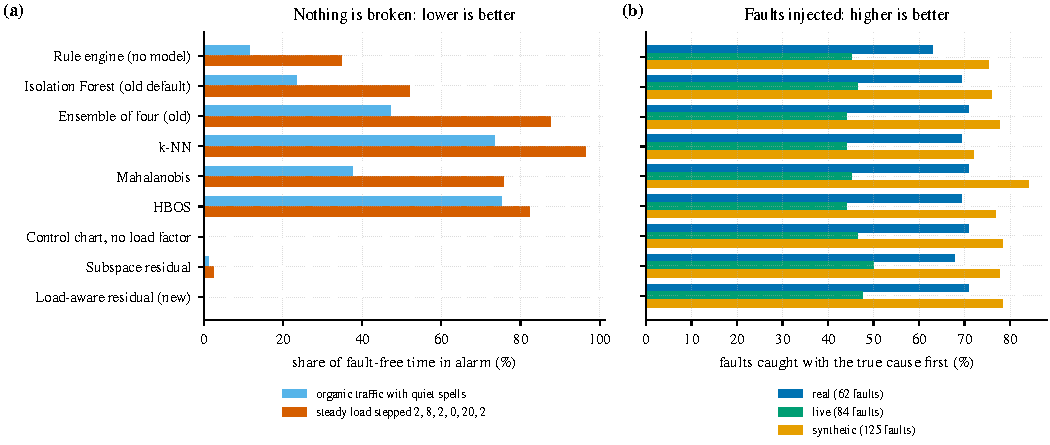
\includegraphics[width=\textwidth]{fig_models.pdf}
\caption[The candidate models on fault-free workload shifts and on injected faults]{The candidate models. (a) Share of fault-free time in alarm on the two workload recordings (lower is better). (b) Share of injected faults caught with the true cause first on the real, live and synthetic sets (higher is better).}
\label{fig:models}
\end{figure}

\begin{enumerate}
\item On injected faults the models are alike. The caught-and-named rate is $68$--$73\%$ on the real faults, $43$--$50\%$ on the live ones and $72$--$84\%$ on the synthetic ones for every candidate; differences of a few points are inside the noise of 62 to 125 faults (the intervals of Table~\ref{tab:main} are $\pm 10$ points). The workload-blind models differ in false alarms: the forest-family detectors raise 4.6 to 34.6 episodes per hour on the real systems and 40.9 to 81.7 on the live ones, against 2.3 and 0.0 for the adopted model.
\item On workload shifts they are not alike. The adopted model is in alarm for 0\% of both recordings; the workload-blind family for 23--75\% and 52--96\%. Replacing the forests by a robust residual with the tail-aware spread is the larger part of the improvement (control chart: 0\% and 0\%); the MAD spread alone is not enough (13\% and 31\%), because it treats bursty signals as Gaussian.
\item The load factor removes what is left. The control chart without it still raises 1.2 and 1.9 false episodes per hour on the two recordings; with it 0.0 and 1.0, and it is the better of the two on the live faults (47.6\% against 46.4\% caught and named). The subspace residual is the strongest alternative (3\% and 4\% of the steady recording in alarm; 50\% caught and named on the live faults). It raises 7.7 to 10.7 false episodes per hour on the steady steps, is slower to adapt, and its cost grows faster than linearly (Section~\ref{sec:cost}).
\end{enumerate}
We therefore adopted the load factor with the tail spread. We report what it does not do: it is not more accurate than the forest on the injected faults (71\% against 69\% on the real ones, inside the noise). A fault that begins during a large change of load can also be masked, because the model then accepts a deviation that either hypothesis about the load explains. Brownouts of nearly idle services remain the open problem for every model (no signal moves), as in the earlier version.

\paragraph{Sensitivity.} Figure~\ref{fig:zline} sweeps the alarm line. A looser line (2 spreads) raises detection to 94\% on the real faults but also the false alarms on the workload recordings (15.0 episodes per hour); a tighter one (6 or 8 spreads) removes all false alarms on the workload recordings but loses detection (87\% and 85\% on the real faults, 83\% and 75\% on the synthetic ones). The adopted line of 4 spreads is the loosest that keeps the workload recordings quiet. The training window (60, 120 or 240 readings) and the slow reference (120, 360 or 720) matter little once they are long enough; a window of 60 readings makes the workload recordings noisy again (10.4 false episodes per hour). We also tried carrying the range guard of the first model over to the residual (a value several floors beyond everything in the window counts as level one): it changed no result on any set of injected faults and added false alarms on the steady-load steps (4.8 episodes per hour at four floors, 1.0 without it), so the adopted model has none.

\paragraph{How fast a mild shift becomes normal.} A deviation that stays between level one and three is accepted as the new normal after $24$ readings (two minutes). Waiting longer, $48$ to $240$ readings, changed nothing on the injected faults (\cn{} $71\%$ on the real ones and $78\%$ on the synthetic ones at every value; synthetic detection $88\%$ against $89$--$90\%$) and nothing on the workload recordings, but doubled the time in alarm on the real systems ($6\%$ to $13\%$) and raised their false alarms from $2.3$ to $3.1$ per hour, because a service whose footprint changes after a restart stays in alarm until it is accepted. The cost of the short setting is that a slow fault that stays only mildly above the line is absorbed after two minutes, as in the simulated slow \texttt{payment} of Section~\ref{sec:engineslive}; a larger shift (level three or more) still needs thirty minutes.

\begin{figure}[!htbp]
\centering
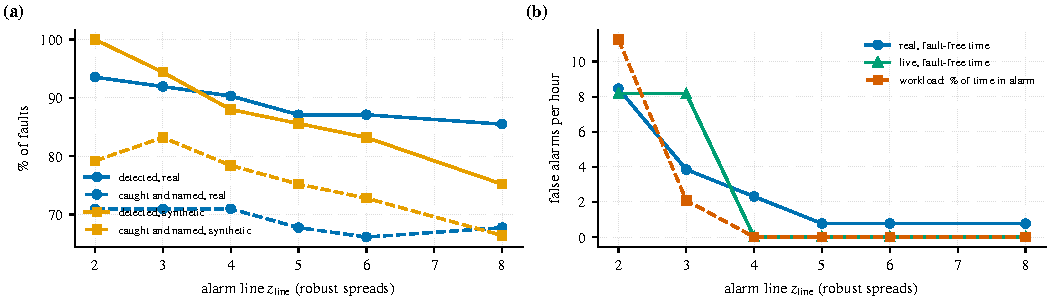
\includegraphics[width=\textwidth]{fig_zline.pdf}
\caption[Sensitivity of the adopted model to its alarm line]{Sensitivity of the load-aware model to its alarm line $z_{\mathrm{line}}$ (the engine alarms at level 2, that is, at $2 z_{\mathrm{line}}$ spreads). (a) Faults detected, and caught and named, on the real and synthetic sets. (b) False alarms per fault-free hour on the real and live sets, and the share of time in alarm on the workload recordings.}
\label{fig:zline}
\end{figure}

\subsection{Rules, the old ML and the new ML side by side}
\label{sec:threeway}
Table~\ref{tab:threeway} puts the three engines a user can pick in the top bar next to each other. The same harness replays them over the same recordings: the rule engine (robust z-score per metric, alarm at three spreads, no model), the first ML engine (per-service Isolation Forests) and the corrected ML engine (load-aware residual). Both ML engines name the source with the same random walk, so any difference between them comes from the model of normal. A longer version with the reasoning in plain words is kept in the repository as \code{wiki/44-ml-comparison.md}.

\begin{table}[!htbp]
\centering
\caption[Rules, old ML and new ML on the same recordings]{The three engines on the same recordings. \cn: faults caught with the true cause named first (\%). FA/h: false-alarm episodes per fault-free hour. Workload columns: share of the fault-free workload recordings spent in alarm (\%). ROC: per-reading AUROC and average precision on the real run and the held-out synthetic set. Cost: mean milliseconds per decision window for 10 and 320 services.}
\label{tab:threeway}
\footnotesize
\setlength{\tabcolsep}{4pt}
\begin{tabular}{lrrr}
\toprule
 & Rules & Old ML (forest) & New ML (load-aware)\\
\midrule
\multicolumn{4}{l}{\emph{Injected faults}}\\
Real, 62 faults: \cn{} / FA/h & 63\% / 9.2 & 69\% / 4.6 & \textbf{71\% / 2.3}\\
Live, 84 faults: \cn{} / FA/h & 45\% / 16.3 & 46\% / 40.9 & \textbf{48\% / 0.0}\\
Synthetic, 125 faults: \cn{} / FA/h & 75\% / 2.6 & 76\% / 0.2 & \textbf{78\% / 0.2}\\
Detected, real / live / synthetic & 90\% / 96\% / 83\% & 87\% / 99\% / 87\% & 90\% / 99\% / 88\%\\
Median delay, real & 15 s & 12 s & 12 s\\
\midrule
\multicolumn{4}{l}{\emph{No fault, only the workload moves}}\\
Organic on/off: time in alarm & 12\% & 23\% & \textbf{0\%}\\
Steps 2--8--2--0--20--2: time in alarm & 35\% & 52\% & \textbf{0\%}\\
\midrule
\multicolumn{4}{l}{\emph{Per-reading ranking}}\\
AUROC / AP, real & 0.69 / 0.34 & 0.63 / 0.29 & 0.66 / 0.31\\
AUROC / AP, synthetic test & 0.87 / 0.67 & 0.86 / 0.53 & 0.84 / 0.66\\
\midrule
Cost, 10 / 320 services (ms) & -- & 8.9 / 296 & 4.0 / 119\\
\bottomrule
\end{tabular}
\end{table}

The table reads in three parts. On injected faults the rule engine catches about as many faults as the ML engines. With container facts ranked first it names the right service for 63\% of the real faults, against 69\% for the old ML and 71\% for the new one. It also raises four times as many false alarms as the new engine on the real run and more than ten times as many on the synthetic set. Every swing of traffic is a deviation to it, and when no container fact is present the loudest service, often a victim, gets the blame. The two ML engines are close on the injected faults; the new one is two points ahead on each set, with fewer false alarms, mostly on the live campaigns, where restarts and traffic pauses are frequent. On the workload recordings the difference is the whole point of the correction: the old ML is in alarm for about half of the steady-load recording, the rule engine for a third of it, and the new ML not at all. Per reading, the rule z-score ranks best on both sets; a single high reading is cheap, and the rule engine loses only once alarms need persistence and a named source. Between the ML engines, the new one has the higher average precision on the held-out set and a slightly lower AUROC, and it is the cheaper of the two.

The new engine differs from the old one in five ways. Before judging any service, it estimates how much the whole project's workload moved and explains that move away. A fault during a load change still shows, because the load is a median that one or two services cannot drag, and a signal counts as normal only if it either ignores the load or follows it. Bursty signals get a fair spread, the engine never learns from readings it alarmed on, and each alarm says which signal moved and by how much. The rules the mapper was built on stay: no labels, no agent on the hosts, only the telemetry the mapper already reads.

\subsection{Detection and root cause}
Table~\ref{tab:main} compares the engines in one harness, now with the corrected ML engine inside. On the real systems the hybrid and the ML engine name the true cause first for 71\% of all faults, against 63\% for the rule layer and 68\% for ranking by anomaly alone. The paired differences are in Figure~\ref{fig:forest}. They are smaller than in the first version of this report and no longer reach significance. Hybrid over rules is $+8.1$ points on the real systems (95\% CI $[-1.6, +17.7]$, $p = 0.117$) and $+5.6$ on the synthetic set ($[-0.6, +11.8]$, $p = 0.093$). Hybrid over the severity ranking is $+3.2$ and $+1.1$ points, and hybrid over the ML engine $0.0$ and $+0.6$. With 62 real faults a difference below about ten points cannot be resolved. What the corrected engine changes is the false-alarm column: the ML engine alarms 2.3 times per fault-free hour on the real systems and 0.2 on the synthetic set, the quietest row, and Section~\ref{sec:workloadres} shows that it stays quiet when only the load moves. The hybrid raises more episodes (6.2 and 0.9) because the rule layer may also trigger it.

\begin{table}[!htbp]
\centering
\caption[Detection and root cause in one harness (point estimates with 95\% bootstrap intervals over faults)]{Detection and root cause in one harness (point estimates with 95\% bootstrap intervals over faults). Det.: faults detected (\%). \acc{1}, \acc{3}: true cause first or in the top three among detected (\%). \cn: caught and named first over all faults (\%). FA/h: false-alarm episodes per fault-free hour. Alarm: share of fault-free time in alarm (\%).}
\label{tab:main}
\footnotesize
\setlength{\tabcolsep}{3pt}
\begin{tabular}{lcccccc}
\toprule
Engine & Det. [95\% CI] & \acc{1} & \acc{3} & \cn{} [95\% CI] & FA/h & Alarm \\
\midrule
\textit{Real benches (62 faults, 217 min)} & & & & & & \\
Rules & 90 [82, 97] & 70 & 91 & 63 [52, 74] & 9.2 & 9 \\
Severity ranking & 90 [82, 97] & 75 & 86 & 68 [56, 79] & 6.2 & 8 \\
ML engine & 90 [82, 97] & 79 & 89 & 71 [60, 81] & 2.3 & 6 \\
\textbf{Hybrid} & 90 [82, 97] & 79 & 89 & 71 [60, 81] & 6.2 & 8 \\
Hybrid + change-point & 95 [89, 100] & 76 & 88 & 73 [61, 82] & 5.4 & 16 \\
Hybrid + learned dir. & 90 [82, 97] & 75 & 89 & 68 [55, 77] & 6.2 & 8 \\
\midrule
\textit{Synthetic held-out (178 faults, 16 topologies)} & & & & & & \\
Rules & 89 [84, 93] & 78 & 95 & 70 [62, 76] & 2.5 & 2 \\
Severity ranking & 93 [89, 97] & 80 & 92 & 74 [67, 80] & 0.9 & 5 \\
ML engine & 92 [87, 96] & 82 & 94 & 75 [69, 81] & 0.2 & 4 \\
\textbf{Hybrid} & 93 [89, 97] & 81 & 93 & 75 [69, 81] & 0.9 & 5 \\
Hybrid + change-point & 94 [90, 98] & 80 & 92 & 75 [69, 81] & 0.8 & 6 \\
Hybrid + learned dir. & 93 [89, 97] & 81 & 93 & 75 [69, 81] & 0.9 & 5 \\
\bottomrule
\end{tabular}
\end{table}

The operating curves (Figure~\ref{fig:op}) show why the comparison is delicate. The engines trade detection for false alarms along nearly overlapping curves. The hybrid and the ML engine sit on or near the upper envelope in both sets, above the rules at almost every false-alarm budget, so their advantage lies in the operating point and not in a single threshold. Figure~\ref{fig:class} breaks C+N down by fault class. The gain over the rules is concentrated in stop faults (16 of 16 against 9 of 16 on the real systems), which is the effect of the \texttt{docker stop} fact, and, on the synthetic set, in flap faults (12 of 12 against 2 of 12).

\begin{figure}[!htbp]
\centering
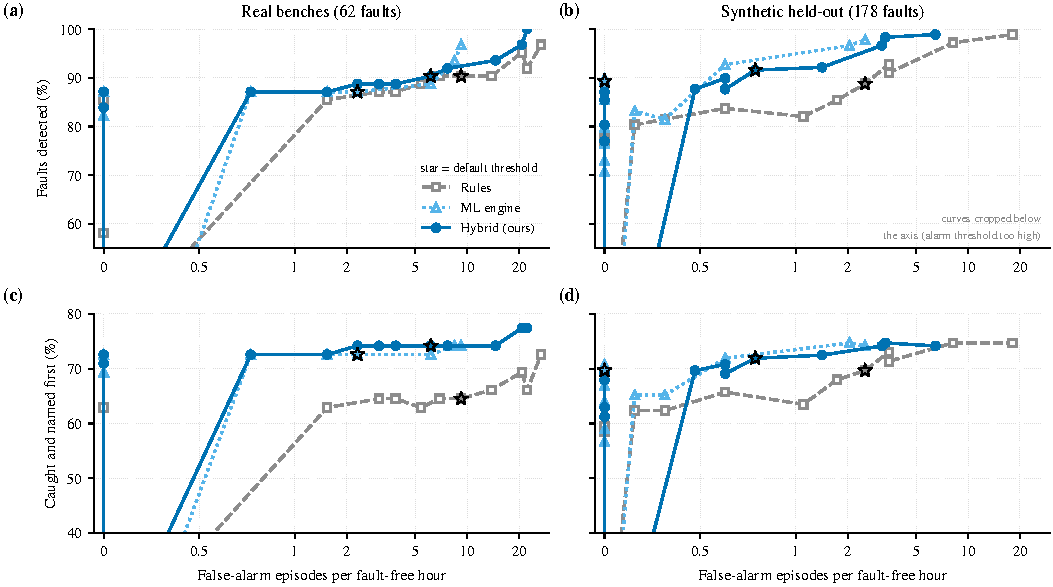
\includegraphics[width=\textwidth]{fig_op.pdf}
\caption[Operating curves. Sweeping the alarm threshold of each engine traces detection rate]{Operating curves. Sweeping the alarm threshold of each engine traces detection rate (top) and caught-and-named rate (bottom) against false-alarm episodes per fault-free hour (symmetric-log axis); stars mark the default threshold. The hybrid sits on the upper envelope in both the real systems (a, c) and the synthetic held-out set (b, d).}
\label{fig:op}
\end{figure}

\begin{figure}[!htbp]
\centering
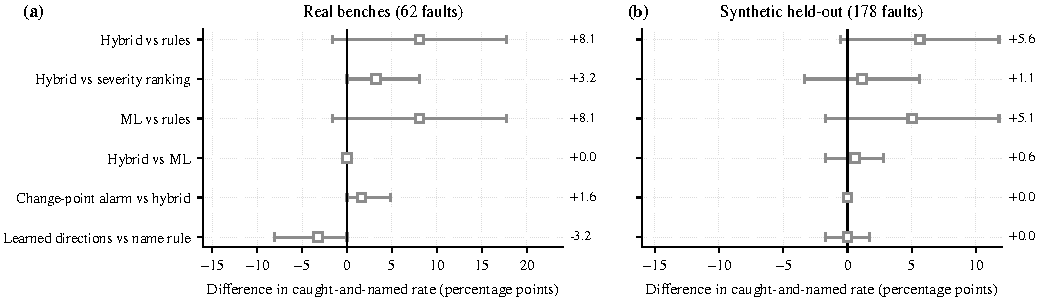
\includegraphics[width=\textwidth]{fig_forest.pdf}
\caption[Paired differences in caught-and-named rate between engines]{Paired differences in caught-and-named rate between engines (percentage points, 95\% paired-bootstrap interval); filled markers exclude zero.}
\label{fig:forest}
\end{figure}

\begin{figure}[!htbp]
\centering
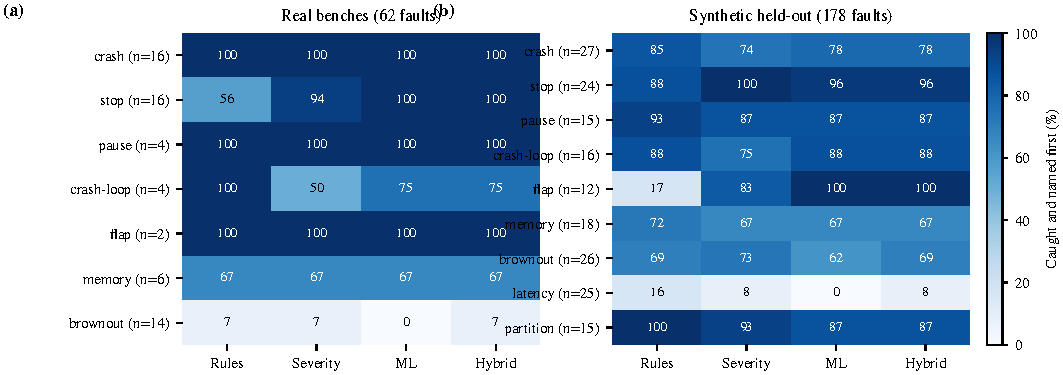
\includegraphics[width=\textwidth]{fig_class.pdf}
\caption[Caught-and-named rate by fault class]{Caught-and-named rate by fault class (percent; $n$ faults per class), for four rankers on the real systems (a) and the synthetic held-out set (b). Brownouts are the open problem on the real systems.}
\label{fig:class}
\end{figure}

\subsection{Which detector}
Table~\ref{tab:roc} scores each model of normal as a service-level classifier, now including the control chart, the subspace residual and the adopted load-aware model. As before, the plain rule $z$-score is as good as or better than every learned detector at separating a faulted service from a healthy one by AUROC (0.695 against 0.629 for the old forest and 0.665 for the load-aware model on the real systems; 0.873 against 0.862 and 0.842 on the synthetic set). On average precision, which weighs the rare faulted services, the load-aware model is above every forest-family detector on both sets (0.313 against at most 0.290 on the real systems; 0.665 against at most 0.608 on the synthetic set). It is level with the rules on the synthetic set (0.666). Separation on the real systems is weak for every detector (AUROC 0.62 to 0.70), because many real faults hit services that are nearly idle.

Discrimination is therefore not what chose the model; behaviour under a change of workload was (Section~\ref{sec:whichmodel}). The adopted model is quiet (alarm time of 6\% against 9\% for the rules on the real systems, Table~\ref{tab:main}); it separates own from symptom evidence; and its alarms complement those of the rules, so their union detects more faults than either on the synthetic set (93\% against 89\%).

\begin{table}[!htbp]
\centering
\caption[Service-level detection by detector (mean $\pm$ s.d]{Service-level detection by model of normal (mean $\pm$ s.d. over three seeds for the randomised detectors; the rule layer and the three residual models are deterministic).}
\label{tab:roc}
\footnotesize
\begin{tabular}{lcccc}
\toprule
 & \multicolumn{2}{c}{Real} & \multicolumn{2}{c}{Synthetic} \\
Detector & AUROC & AP & AUROC & AP \\
\midrule
Rule z-score & 0.695$\pm$0.000 & 0.337$\pm$0.000 & 0.873$\pm$0.000 & 0.666$\pm$0.000 \\
Isolation Forest (old) & 0.629$\pm$0.004 & 0.288$\pm$0.003 & 0.862$\pm$0.004 & 0.528$\pm$0.020 \\
k-NN & 0.668$\pm$0.010 & 0.193$\pm$0.004 & 0.860$\pm$0.001 & 0.517$\pm$0.004 \\
Mahalanobis & 0.650$\pm$0.003 & 0.290$\pm$0.004 & 0.868$\pm$0.001 & 0.608$\pm$0.006 \\
HBOS & 0.620$\pm$0.005 & 0.274$\pm$0.006 & 0.853$\pm$0.004 & 0.473$\pm$0.030 \\
Ensemble of four & 0.650$\pm$0.006 & 0.287$\pm$0.009 & 0.865$\pm$0.001 & 0.593$\pm$0.002 \\
Control chart (no load factor) & 0.669$\pm$0.000 & 0.302$\pm$0.000 & 0.842$\pm$0.000 & 0.657$\pm$0.000 \\
Subspace residual & 0.696$\pm$0.000 & 0.298$\pm$0.000 & 0.847$\pm$0.000 & 0.629$\pm$0.000 \\
Load-aware residual (new) & 0.665$\pm$0.000 & 0.313$\pm$0.000 & 0.842$\pm$0.000 & 0.665$\pm$0.000 \\
\bottomrule
\end{tabular}
\end{table}

\subsection{Detection delay and root-cause depth}
Figure~\ref{fig:delay} shows detection delay as a cumulative distribution. On the real systems the hybrid's median delay is 11.3\,s against 14.9\,s for the rules, and the change-point alarm lifts the detected fraction from 90\% to 95\% and moves the median to 4.8\,s. On the synthetic set, whose faults are abrupt, the curves almost coincide (8.2\,s against 9.5\,s for the rules). The change-point alarm has a price visible in Table~\ref{tab:main}: alarm time rises from 8\% to 16\% on the real systems. In the top $k$ (the \acc{1} and \acc{3} columns of Table~\ref{tab:main}) the ML-based rankers reach the true cause first more often than the rules on the real systems (79\% against 70\% of the detected faults), and the rankers converge by $k = 3$ near the 90\% detection ceiling, so the remaining misses are mostly faults the engine does not see (brownouts on near-idle services), and few are faults it ranks badly.

\begin{figure}[!htbp]
\centering
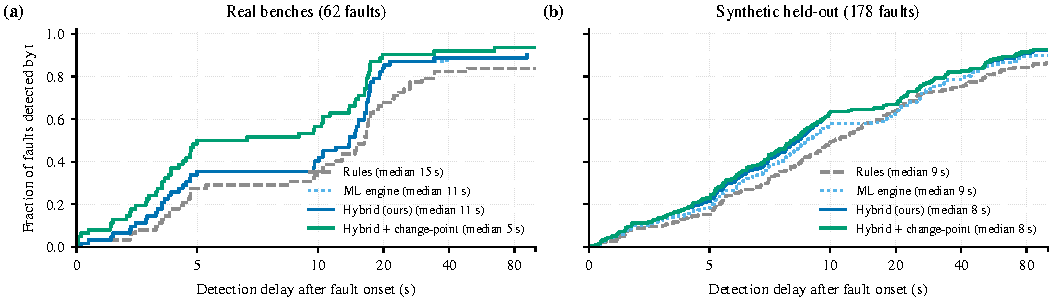
\includegraphics[width=\textwidth]{fig_delay.pdf}
\caption[Detection delay after fault onset as a cumulative distribution]{Detection delay after fault onset as a cumulative distribution (symmetric-log axis); legends give the median over detected faults. The curves plateau at each engine's detection rate.}
\label{fig:delay}
\end{figure}

\subsection{Ablation}
\label{sec:ablation}
Figure~\ref{fig:abl} removes one mechanism of the corrected ML engine at a time. The most important single component is still the \code{docker stop} fact: without it \cn{} falls by 18 points on the real systems and 15 on the synthetic set, because every stopped service goes unnamed. The crash-loop fact (0 and 7 points) and the random walk (3 and 2 points) each contribute. Two mechanisms act on the contract rather than on accuracy. Without the load factor nothing changes on injected faults (the load does not move in them) and the effect appears only on the workload recordings of Section~\ref{sec:workloadres}: false alarms rise from 0.0 to 1.2 and from 1.0 to 1.9 per hour there. With the MAD spread instead of the tail-aware one, alarm time on the real systems doubles (6\% to 12\%) and, on the workload recordings, rises from 0\% to 10\% and 6\% (13\% and 31\% when the load factor is also removed). Removing the one-sided features raises alarm time on the real systems from 6\% to 24\%; the two-speed drift keeps it at 6\% instead of 13\% and false alarms at 2.3 instead of 3.1 per hour. Alarming at level one instead of two raises \cn{} by 2 points on both sets but more than doubles the false alarms on the real systems (5.4 per hour). The one-sided features do not matter on the synthetic set, where restarts do not lower memory: an effect of the real systems that the simulator does not reproduce. The range guard of the first version has no counterpart: the robust spread takes its place.

\begin{figure}[!htbp]
\centering
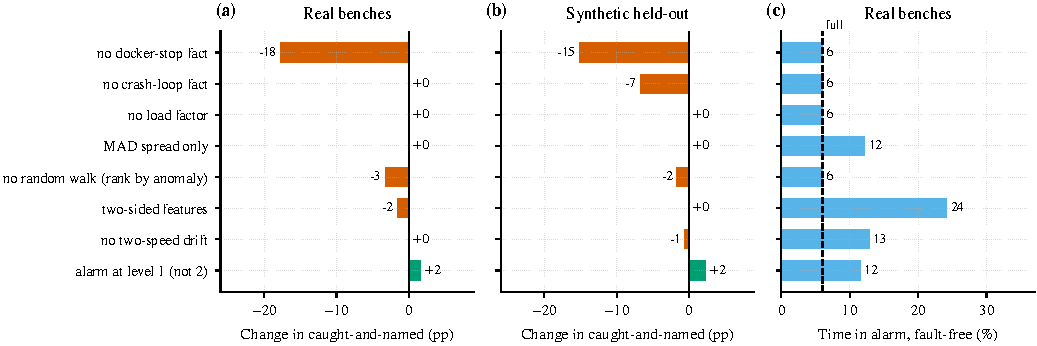
\includegraphics[width=\textwidth]{fig_ablation.pdf}
\caption[Ablation. Each bar removes one mechanism from the full engine.]{Ablation of the corrected ML engine. Each bar removes one mechanism from the full engine. (a), (b): change in caught-and-named rate (percentage points) on the real systems and the synthetic held-out set. (c): share of fault-free time in alarm on the real systems; the dashed line marks the full engine.}
\label{fig:abl}
\end{figure}

\subsection{When does the graph matter? The amplification study}
Standard benchmarks have faults whose own service is also the loudest, which is the case where ranking by severity cannot fail. To probe the regime in which it can, soft faults (brownout, latency, memory) were regenerated with the amplification factor $A \in \{1, 1.5, 2, 3, 4\}$, the hybrid's alarms were kept identical for every ranker, and only the ranking varied (Figure~\ref{fig:amp}). As $A$ grows, the share of faults in which some victim is louder than the true cause rises from 10\% to 21\% (panel c), the severity ranking falls from 76\% to 71\%, and the walk holds at 75 to 76\%. The gain of the walk over severity therefore grows from zero to $+3.8$ points (95\% CI $[-0.9, +9.4]$ at $A = 4$) and that of the walk with learned directions to $+4.7$ ($[-0.9, +10.4]$) (panel b). The intervals include zero at every level. In the first version of the study the own-versus-explained decomposition of the rule layer was the strongest ranker on soft faults; with the corrected ML engine it is not (71 to 75\%, $-1.9$ to $0.0$ points against severity, intervals including zero), because the engine's own and symptom levels now carry the same separation. A router that uses it whenever no container fact holds did not change the full benchmarks (within $\pm 2$ points), so the shipped ranking is unchanged. Graph-aware ranking remains a modest, regime-dependent gain that this sample is too small to confirm.

\begin{figure}[!htbp]
\centering
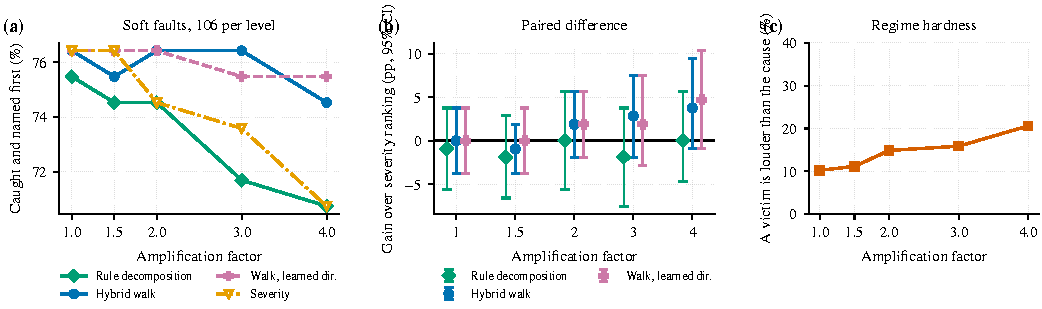
\includegraphics[width=\textwidth]{fig_amp.pdf}
\caption[Amplification study on soft faults (106 per level)]{Amplification study on soft faults (106 per level). (a) Caught-and-named rate of four rankers on identical alarms. (b) Gain over the severity ranking with 95\% paired-bootstrap intervals. (c) Share of faults in which a victim is louder than the true cause.}
\label{fig:amp}
\end{figure}

\subsection{The cascade model}
Figure~\ref{fig:cal} evaluates who-is-next predictions at the first alarm of each fault: for every service still healthy, the probability that it turns unhealthy before the fault ends. On the synthetic set (163 faults, 1\,289 predictions, 69 cascades) the learned propagation model reaches AUROC 0.841 against 0.827 for the same noisy-OR with every edge fixed at 0.7, a Brier score of 0.047 against 0.052 and an ECE of 0.033 against 0.051. The calibration is better than that of the fixed model, the ranking only slightly. The reliability curve is noisy in the upper bins, which hold few predictions. \emph{On the real systems the experiment cannot be done well:} only 10 of 535 predictions were followed by a cascade (56 faults), so the real-system comparison (AUROC 0.742 against 0.633; the live mapper's own risk values 0.591) is not informative. The real faults are mostly single-service outages that the systems absorb; whether learned propagation helps on a real cascade is untested.

\begin{figure}[!htbp]
\centering
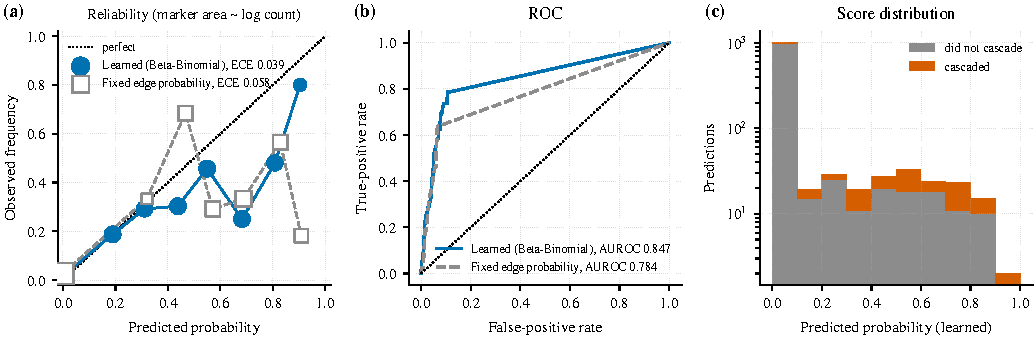
\includegraphics[width=\textwidth]{fig_calibration.pdf}
\caption[Who-is-next prediction on the synthetic held-out set]{Who-is-next prediction on the synthetic held-out set. (a) Reliability diagram with equal-width bins and marker area proportional to the logarithm of the bin count. (b) ROC curves. (c) Distribution of the learned predicted probabilities.}
\label{fig:cal}
\end{figure}

\subsection{Learned directions}
Figure~\ref{fig:dirs} reports direction accuracy on observed pairs that are true calls. With names available the name rule is correct for 21 of 31 real pairs (and leaves 10 undecided); the learned rule is correct for 27 of 31 (4 wrong). With service names hidden the name rule is undecided for every pair while the learned rule is unchanged; the same holds on the synthetic set (95 of 204 against 198 of 204 correct). The effect on ranking is smaller than The effect on directions. With names available the learned directions do \emph{not} beat the name rule (68\% against 71\% on the real systems, $-3.2$ points, not significant). With names hidden they reach 68\% against 66\% for the name rule and 71\% for the true graph. Learned directions are a robustness mechanism, not an accuracy gain.

\begin{figure}[!htbp]
\centering
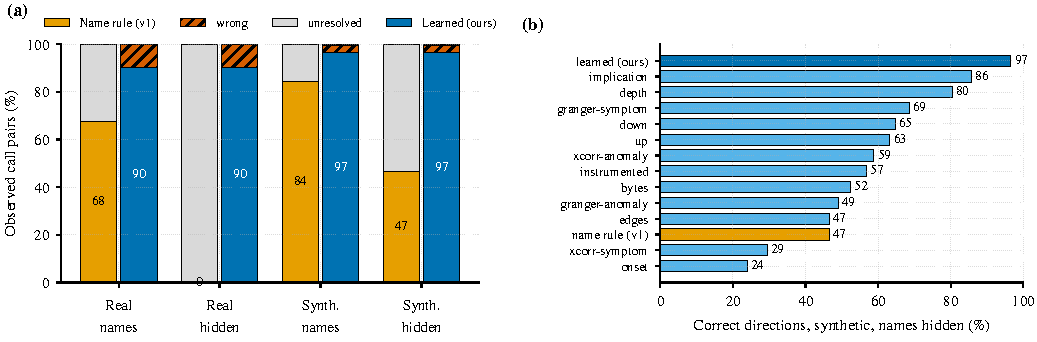
\includegraphics[width=\textwidth]{fig_dirs.pdf}
\caption[Call directions: name rule against learned rule]{Call directions. (a) Share of observed true-call pairs oriented correctly, wrongly, or left unresolved by the name rule and by the learned rule, with service names shown or hidden. (b) Correct share of each individual signal on the synthetic set with names hidden.}
\label{fig:dirs}
\end{figure}

\subsection{Early warning and fault diagnosis}
The trend forecast (now a straight line through the recent deviations from what the load predicts) warns before the alarm for 13 of 178 synthetic faults (7 of 18 memory leaks, 4 of 25 latency faults, 2 of 26 brownouts) with a median lead of 25\,s and 0.8 false warning episodes per fault-free hour (Figure~\ref{fig:early}); the first version, on the raw readings, warned for 16 (5 of 26 brownouts). On the real systems it fired before the alarm for none of the 62 faults, since those faults are abrupt, and raised 6.9 false warning episodes per hour; early warning of gradual faults is the weakest part of the system and is reported as such. Figure~\ref{fig:diag} shows fault-type diagnosis. With the true service the forest is correct for 99\% of synthetic faults 60\,s after the alarm; on the engine's own suspect it is 79\%, because a wrong suspect is rarely typed correctly. On the real systems a hand-written decision list generalises best (64\% on the suspect, 84\% on the true service), because real flaps are pause cycles and real brownouts on idle services show no throttling: differences between the simulator and the real systems that the learned models absorb as synthetic-specific patterns.

\begin{figure}[!htbp]
\centering
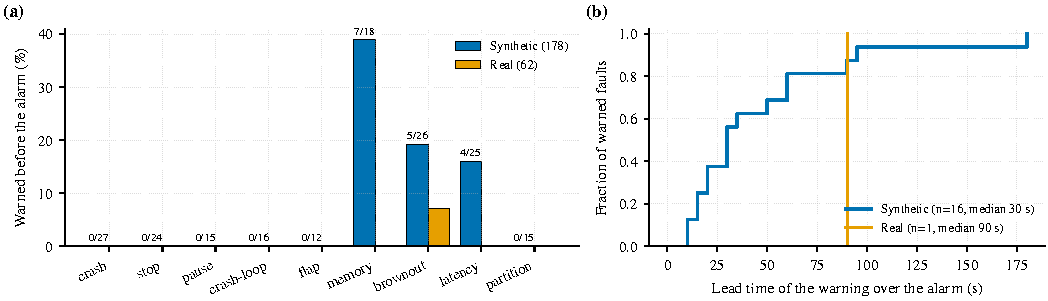
\includegraphics[width=\textwidth]{fig_early.pdf}
\caption[Early warning by fault class and lead time]{Early warning. (a) Share of faults warned before the alarm, by fault class. (b) Lead time of the warnings over the alarm as a cumulative distribution.}
\label{fig:early}
\end{figure}

\begin{figure}[!htbp]
\centering
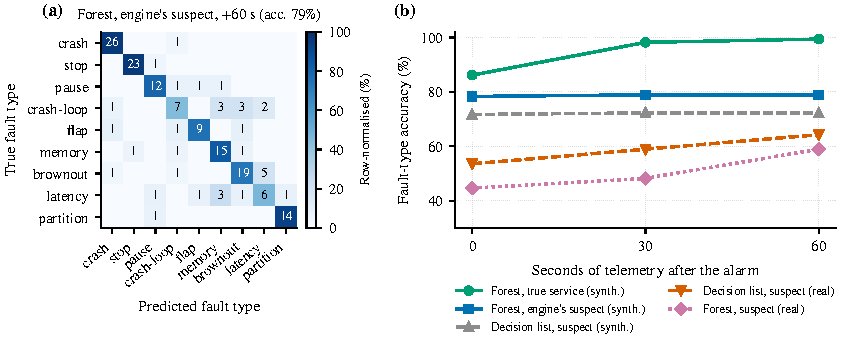
\includegraphics[width=\textwidth]{fig_diag.pdf}
\caption[Fault-type diagnosis]{Fault-type diagnosis. (a) Confusion matrix (counts; shading is row-normalised) of the random forest on the engine's suspect 60\,s after the alarm, synthetic held-out set. (b) Accuracy against seconds of telemetry after the alarm, for the true service and the engine's suspect.}
\label{fig:diag}
\end{figure}

\subsection{Cost}
\label{sec:cost}
The pipeline is unsupervised, needs no GPU and runs on one core. Figure~\ref{fig:scale} times one complete decision window (container facts, the model of normal, random walk, forecast) on random call graphs of 10 to 320 services, after a warm-up long enough for every service to have a model. The adopted load-aware model costs about $0.37$\,ms per service per window and grows linearly: 4.0\,ms for 10 services, 26.8\,ms for 80 and 119\,ms for 320 (95th percentile 356\,ms), always far below the 5\,s collection period. The old forest cost about $0.9$\,ms per service (296\,ms for 320) with 95th-percentile windows nine times the mean, because every service refits at once every ten readings. The load-aware model refreshes its baselines every four readings with a much smaller peak (about three times the mean). The subspace residual grows faster than linearly (1.2\,s for 320 services, with 11\,s windows at the 95th percentile) because its covariance has one row per service-signal pair. On the two benches (12 and 13 services) a window takes about 5\,ms. These are wall-clock times on one core of a shared four-core virtual machine, not a tuned benchmark.

\begin{figure}[!htbp]
\centering
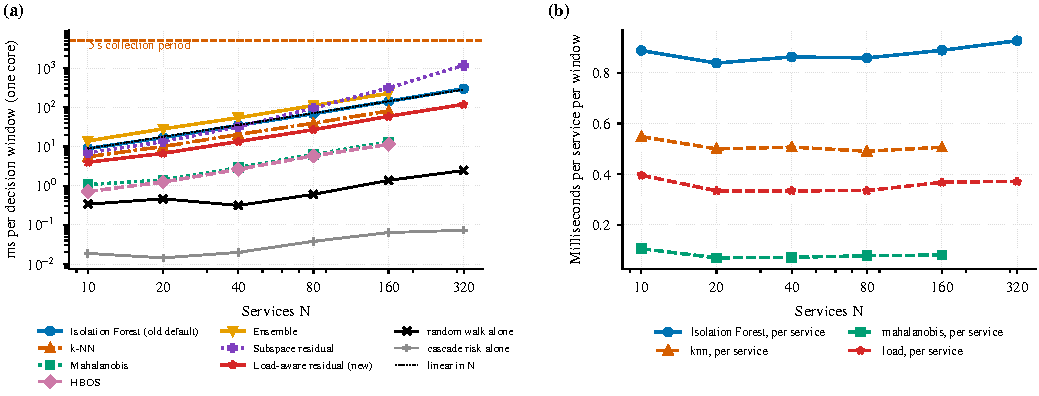
\includegraphics[width=\textwidth]{fig_scale.pdf}
\caption[Cost of one decision window against the number of services]{Cost of one decision window against the number of services (single core, logarithmic axes; the dashed line is the 5\,s collection period). (a) Mean milliseconds per window for each model of normal, the random walk and the cascade risk alone. (b) Milliseconds per service per window.}
\label{fig:scale}
\end{figure}

\subsection{Case studies}
Figure~\ref{fig:case} shows three real incidents, chosen by class before looking at the outcome. In (a) a memory leak overlaps several outages: the engine names the stopped containers first, as it should, and only a model of concurrent faults could do better. In (b) a crash loop is named correctly about 30\,s after its first kill and stays named between kills. In (c) a brownout on an almost idle service never raises an alarm, which is the open problem of Figure~\ref{fig:class}.

\begin{figure}[!htbp]
\centering
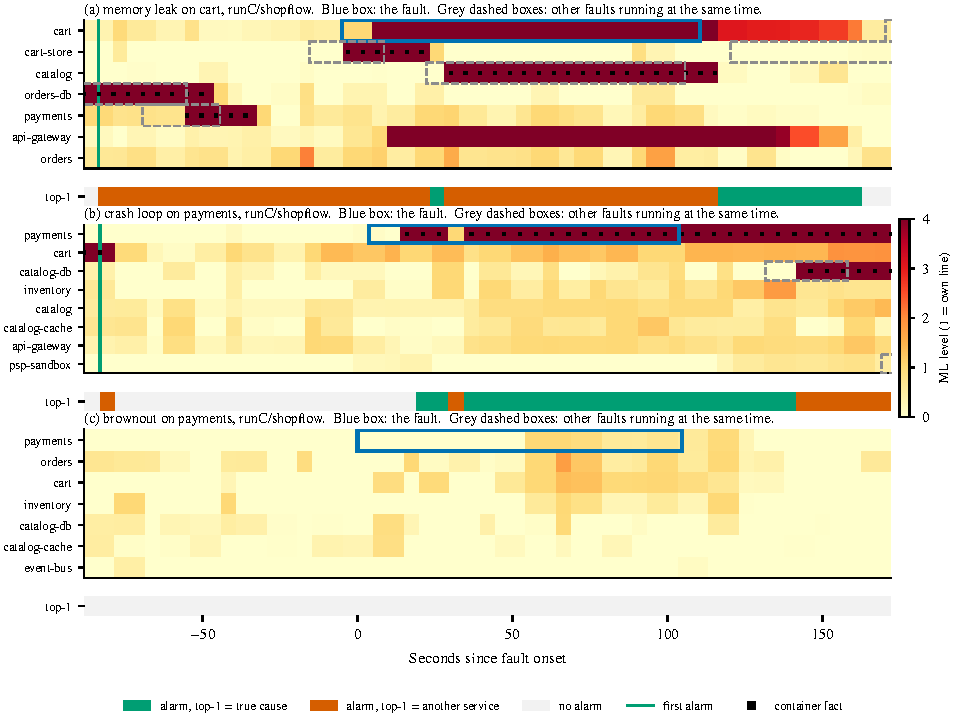
\includegraphics[width=0.86\textwidth]{fig_case.pdf}
\caption[Three real incidents]{Three real incidents. Heat maps show the ML level of the most relevant services; the blue box is the fault, grey dashed boxes are other faults running at the same time, black squares mark container facts, the green line is the first alarm in the window (an alarm already ongoing from an earlier fault starts at the left edge), and the strip below each map shows whether the engine's top-ranked service was the true cause.}
\label{fig:case}
\end{figure}

\subsection{The three engines on one live fault}
\label{sec:engineslive}
To show what the Detection engines page adds, the simulator was run with a slow \texttt{payment} service (CPU saturated at 97\% from second 30 of the fault run; \texttt{orders} follows at 86\% twelve seconds later), the ground-truth root cause being \texttt{payment}. The three engines were read every four seconds through the page's API after a 260-second quiet period (Table~\ref{tab:live}).
\begin{table}[!htbp]
\centering
\caption[One simulated fault: each engine's first suspect over time]{One simulated fault (slow \texttt{payment}): each engine's first suspect and its peak against its own alarm line, at three moments after the onset. The simulator reports every two seconds, so 24 readings are 48 s here (two minutes on a real host).}
\label{tab:live}
\footnotesize
\renewcommand{\arraystretch}{1.2}
\begin{tabular}{l>{\raggedright\arraybackslash}p{0.22\textwidth}>{\raggedright\arraybackslash}p{0.3\textwidth}>{\raggedright\arraybackslash}p{0.22\textwidth}}
\toprule
\textbf{Engine} & \textbf{+5 s: payment only} & \textbf{+20 to +70 s: both saturated} & \textbf{after +75 s}\\
\midrule
Rules & payment (3.0$\times$) & orders (3.7$\times$), payment second (3.0$\times$) & the same\\
ML & payment (88\% of the walk), peak 1.3 & payment (57\%), orders (43\%), peak 1.3 & absorbed: no alarm\\
Hybrid & payment & payment (0.91), orders (0.87) & orders (alarm kept by the rules)\\
\bottomrule
\end{tabular}
\end{table}
This is one simulated fault and an illustration, not evidence. It shows the mechanism the evaluation measures at scale: the rule layer ranks the loudest service first, so it blames \texttt{orders} as soon as both are saturated, while the ML engine lets the walk keep the blame on the source. It also shows the price of the two-minute drift rule (Section~\ref{sec:whichmodel}): a saturation that lasts longer than the acceptance time is absorbed as the new normal and the ML alarm clears. The hybrid keeps alarming because of the rule layer, but its ranking then follows the rules.

\subsection{Operational findings from the benchmark hosts}
\label{sec:hostfindings}
Operating the benchmark hosts produced three findings that changed the tools.
\begin{itemize}
\item A host too small for its workload looks like a mapper fault. The OpenTelemetry demo ran on a 2-vCPU, 4 GiB instance, with a load average of about 25 and 3.6 of 3.8 GiB of memory in use, no swap, and Docker did not answer within 25 seconds; the dashboard showed no services. A second host with 4 GiB of swap and a load average of 0.2 ran 27 containers of a social-network benchmark normally. The lesson is operational: the mapper depends on the host's Docker daemon answering, and a host that cannot answer shows nothing. The check tool now says so in one step.
\item Idle front ends have no edges. On a healthy social-network host, the front-end containers showed no outgoing sockets when sampled, because nothing was calling them; an undeclared edge expires ten minutes after its last traffic. A front end that is idle therefore has no edge until traffic arrives, which is correct behaviour but looks like a fault. Declared edges from the Compose file keep an idle link on the screen.
\item Hard-coded project names blocked traffic; the traffic controller accepted only five named projects, so benchmark hosts with other names could not be driven. Unknown projects now get a generic workflow.
\end{itemize}


\section{Live Fault Lab Experiments: Auto-restart On and Off}
\label{sec:live}
The 62-fault evaluation above was made on recorded campaigns. To test the mapper once more against a system it cannot see into, and to settle whether its optional auto-restart changes the results, both benchmark benches (Section~\ref{sec:benches}) were run live inside Docker, reached by the mapper over SSH exactly like a remote host (auto-restart exists only on that path). The Fault Lab replayed the \emph{same} plan every time (seed 11, the \texttt{stormy} profile, crash, stop, pause and brownout faults, 18 minutes, 21 faults), once with \texttt{MAPPER\_AUTO\_RESTART} on and once with it off, after a 6-minute warm-up. The hybrid engine decided the incidents and the harness scored them against the injector's private ledger. Only one bench ran at a time. The run scripts and every recorded file are in the repository (\texttt{run/scripts/autorestart-experiment.sh}, \texttt{run/recorded-runs/autorestart/}).

\begin{table}[!htbp]
\centering
\caption{Live campaigns, same fault plan, auto-restart on and off (21 faults each; 95\% Wilson intervals).}
\label{tab:livecampaign}
\small
\renewcommand{\arraystretch}{1.2}
\begin{tabular}{llrrrrr}
\toprule
\textbf{Bench} & \textbf{Auto-restart} & \textbf{Detected} & \textbf{Top-1 (\%)} & \textbf{Top-3 (\%)} & \textbf{Delay (s)} & \textbf{FA/h}\\
\midrule
ShopFlow & on  & 100\% & 33 [17, 55] & 71 [50, 86] & 3.3 & 9.2\\
ShopFlow & off & 100\% & 24 [11, 45] & 71 [50, 86] & 2.6 & 0.0\\
LedgerLine & on  & 95\% & 55 [34, 74] & 65 [43, 82] & 9.7 & 0.0\\
LedgerLine & off & 95\% & 40 [22, 61] & 70 [48, 85] & 3.9 & 3.1\\
\bottomrule
\end{tabular}

\smallskip
{\footnotesize Delay is the median time from fault onset to the first alarm; FA/h is false-alarm episodes per fault-free hour.}
\end{table}

\begin{table}[!htbp]
\centering
\caption{Top-1 and Top-3 root-cause accuracy (\%) by fault class in the live campaigns (on / off).}
\label{tab:liveclass}
\small
\renewcommand{\arraystretch}{1.15}
\begin{tabular}{lrrrr}
\toprule
 & & & \textbf{ShopFlow} & \textbf{LedgerLine}\\
\textbf{Fault class} & \textbf{Faults} & & \textbf{Top-1 / Top-3} & \textbf{Top-1 / Top-3}\\
\midrule
Brownout & 6 & on / off & 0 / 17 \hspace{4pt} 0 / 0 & 0 / 0 \hspace{4pt} 0 / 20\\
Crash & 6 & on / off & 33 / 83 \hspace{4pt} 33 / 100 & 80 / 80 \hspace{4pt} 33 / 83\\
Pause & 7 & on / off & 57 / 100 \hspace{4pt} 29 / 100 & 86 / 100 \hspace{4pt} 86 / 100\\
Stop & 2 & on / off & 50 / 100 \hspace{4pt} 50 / 100 & 50 / 100 \hspace{4pt} 0 / 50\\
\bottomrule
\end{tabular}
\end{table}

\textbf{What the numbers show.} Every fault but one was detected in both systems, and the true cause was within the top three suspects in 65 to 71\,\% of the faults. The differences between the on and off rows are 9 and 15 points of Top-1, and the false-alarm column moves in opposite directions (more with auto-restart on in ShopFlow, fewer in LedgerLine). With 21 faults the intervals overlap completely, so none of these differences can be called an effect of auto-restart. Brownouts are the weak class in all four runs (no Top-1 at all), which agrees with the 62-fault results of Section~\ref{sec:resultsmain}.

\textbf{Why there was no effect to find.} The log of each run shows what auto-restart actually did. It restarted no container of the bench under test. The one restart in each ``on'' run was of the \emph{other} bench's message bus, which had been stopped by hand to keep one bench per run and which exited with code 1; the mapper, which sees every container on the host, restarted it. That is an artefact of the setup and is reported as such. Three properties of the mapper and the benches explain the rest:
\begin{itemize}
\item the benches set \texttt{restart: always}, so Docker brings a crashed container back within seconds, before the mapper's next pass;
\item the mapper only looks for dead containers once per discovery cycle (180\,s), longer than the 20-second crash faults;
\item it skips containers that exited with code 0, and a container stopped with \texttt{docker stop} exits with code 0.
\end{itemize}

\begin{sloppypar}
\textbf{A direct test with long outages.} To give auto-restart a chance to act, \texttt{cart} and \texttt{payments} were each stopped for 5 minutes by the Fault Lab (\texttt{run/scripts/autorestart-stop-test.sh}), with the state of each container sampled every 2 seconds. Table~\ref{tab:stoptest} shows no difference: the mapper left the containers down in both modes.
\end{sloppypar}

\begin{table}[!htbp]
\centering
\caption{Time a stopped container stayed down, with auto-restart on and off (injector releases it after 300\,s).}
\label{tab:stoptest}
\small
\begin{tabular}{lrr}
\toprule
\textbf{Container} & \textbf{On (s)} & \textbf{Off (s)}\\
\midrule
cart & 299 & 298\\
payments & 301 & 301\\
\bottomrule
\end{tabular}
\end{table}

\textbf{Conclusion.} On these benchmarks auto-restart is inert: it neither helped nor hurt detection or root-cause accuracy beyond run-to-run variation, and the rule that skips exit code 0 means a deliberate stop is never undone. It would matter on a host whose containers have no restart policy and exit with a failure code, which these benches do not model, so that case is untested. Switching it off for evaluation remains the safe default, because the mapper then cannot heal what the injector breaks.

\section{Analysis}
\textbf{What the evidence supports.} The first ML engine mistook a change of workload for a fault: on fault-free recordings it sat in alarm for 23 to 52\% of the time, and every workload-blind detector we tried did the same or worse (Section~\ref{sec:workloadres}). The load-aware model that replaced it stays quiet on both recordings and loses nothing on injected faults. Container facts carry more weight than any other component; the ablation costs 18 and 15 points when the \code{docker stop} fact goes. And learned propagation calibrates better than fixed edge probabilities on observed cascades (ECE 0.033 against 0.051, AUROC 0.841 against 0.827).

\textbf{What did not work.} Several expected gains never appeared. The corrected engine is no more accurate than the first on injected faults. Hybrid over rules was significant in the first version ($+9.7$ points, $p = 0.032$) and is not now ($+8.1$, $p = 0.117$), so the improvement sits in robustness, not in the benchmark score. The random walk does not beat ranking by anomaly alone, learned directions do not beat the name rule when names exist, and onset-precedence re-ranking changed nothing. The subspace residual, the principled multivariate alternative, discriminates as well as the adopted model but raises more false alarms on the load steps and costs more. We report these because an operator gains more from a pipeline that states where it stops. The plain rule $z$-score remains a strong detector. The load-aware model earns its place by staying quiet under changing load and by catching faults the rules miss, not by separating faulted services better.

\textbf{The measurement bugs.} Before we fixed the ledger reader, every engine scored against only part of the real faults (14 of 31 per system stayed hidden), and the outages of the hidden faults counted as false alarms. Every number in this report therefore uses all 62 faults, and a regression test guards the reader. A second bug in the replay (Section~\ref{sec:bug2}) deleted the idle stretches from the recordings. That bug explains why the benchmarks never exposed the first ML engine's failure; an operator found it on a live system. Both bugs flattered the engines.

\section{Discussion and Threats to Validity}
\textbf{Construct validity.} The injector's ledger is the ground truth. It names the structural root cause and the services able to suffer. Whether a service visibly suffers depends on protections the ledger does not model, so cascade recall understates true propagation. The offline recordings keep no edge evidence, which leaves the evidence weighting of Section~\ref{sec:graph} unmeasured.

\textbf{Internal validity.} The authors chose the settings. We swept the alarm line, window and slow reference of the load-aware model over all recordings together (Figure~\ref{fig:zline}), which amounts to tuning on test data; the adopted values sit in the sweep's flat region, not at its maximum. On the synthetic track a disjoint tuning split picked the settings and the test split was scored once. On the real track no held-out system exists, so the real numbers run optimistic by an unknown margin. We found the two container facts by inspecting the real runs.

\textbf{External validity.} Two real applications, one capture and live recordings on one machine limit the claim. Generators produced the workload recordings (organic or closed-loop), so a real day of users stays untested, and a fault that begins during a large change of load can hide behind the load-aware model. Architecture independence rests on the cross-system check and on synthetic topologies. It is argued, not proven. The simulator is also cleaner than a real system: restarts do not lower memory in it.

\textbf{Conclusion validity.} With 62 real faults, no difference below about ten points is resolvable, and overlapping faults make the intervals optimistic. The workload claims rest on four fault-free recordings of 62 and 72 minutes. The effect is large (0\% against 23 to 96\% of the time in alarm), but four recordings are few.

\textbf{Auto-restart.} The mapper can restart crashed containers on a target (Section~\ref{sec:tools}, Chapter~\ref{ch:system}). Live campaigns with the feature on and off showed no effect on these benches (Section~\ref{sec:live}). Even so, switch it off for evaluation runs so the mapper cannot heal the faults the injector applies.

\section{Comparison with Existing Approaches}
The published methods in Table~\ref{tab:litreview} were not re-implemented on our recordings, so there is no head-to-head accuracy table against them. What is compared head to head are the baselines that those methods build on: the rule layer, ranking by anomaly alone (the severity ranking), the walk, and the ML engine in its two versions. Table~\ref{tab:vsexisting} sets the measured results beside the qualitative properties of Chapter~\ref{ch:lit}.

\begin{table}[!htbp]
\centering
\caption{This project beside the approaches it builds on. Accuracy figures are caught-and-named on the 62 real faults.}
\label{tab:vsexisting}
\small
\renewcommand{\arraystretch}{1.25}
\begin{tabularx}{\textwidth}{>{\raggedright\arraybackslash}p{3.7cm}>{\raggedright\arraybackslash}p{2.0cm}>{\raggedright\arraybackslash}X}
\toprule
\textbf{Approach} & \textbf{C+N (real)} & \textbf{Notes}\\
\midrule
Rule layer (z-score) & 63\% & Fast, 9 false-alarm episodes per hour, 9\% alarm time\\
Severity ranking (loudest service) & 68\% & Cannot fail when the cause is loudest; weakens as victims get louder\\
Per-service Isolation Forest + walk (first version) & 69\% & 4.6 false alarms per hour; in alarm for 23 to 52\% of the time when only the load moves\\
ML engine (load-aware model + walk) & 71\% & Fewest false alarms (2.3 per hour), 6\% alarm time; 0\% when only the load moves\\
\textbf{Hybrid (this project)} & \textbf{71\%} & Paired $+8.1$ points over rules (not significant); names stops 16 of 16\\
Learned fusion methods \cite{zhang2023diagfusion,sun2024deephunt,lee2023eadro} & not run & Need labelled failures and GPU; not auditable\\
Trace-based rankers \cite{yu2021microrank} & not run & Need tracing in every service\\
\bottomrule
\end{tabularx}
\end{table}

\section{Significance and Implications}
An instrumentation-free tool can recover a usable call graph and a useful ranking, and for small teams that is the difference between having a diagnosis tool and not. Container facts are worth more than any statistical refinement: a stopped container is something one knows, and folding it into an anomaly score throws information away. And the right operating contract for an alarm is the one the operator experiences, which is why alarm time is reported beside false-alarm episodes.

\clearpage
\chapter[CONCLUSION AND FUTURE SCOPE]{Conclusion and Future Scope}
\label{ch:conclusion}

\section{Summary of Work}
The project built an instrumentation-free platform that watches containerised microservices from outside, recovers their call graph, and runs an unsupervised diagnosis pipeline on it. A collector agent reads Docker state, statistics and socket tables over SSH; an evidence-weighted graph orients each edge by its listening port; a hybrid detector of per-service Isolation Forests and a robust rule layer treats container facts as evidence; a ranker splits each deviation into what neighbours explain and what they do not and runs a random walk over the call graph; a cascade model with learned Beta--Binomial edge probabilities predicts who is next. A dashboard shows the result in 2D and 3D, and a Detection engines page runs Rules, ML and Hybrid in parallel and shows what each detected, computed and predicted. The system was evaluated on 62 faults injected blind into two real containerised systems and on 178 held-out synthetic faults, and operated on further benchmark applications on EC2.

\section{Conclusions}
\begin{enumerate}
\item On 62 real faults the hybrid names the true cause first for 74\% against 65\% for the rule layer (paired $+9.7$ points, 95\% CI $[+1.6,+17.7]$, $p=0.032$); on the synthetic set the difference is not significant ($+2.2$ points).
\item The container facts are the most valuable single component: removing the \code{docker stop} fact costs 19 points on the real systems and 16 on the synthetic set.
\item Learned propagation discriminates better than fixed edge probabilities on 80 observed cascades (AUROC 0.847 against 0.784), with a lower Brier score and a lower expected calibration error. On the real systems the experiment is uninformative because almost no real fault cascaded.
\item Learned directions stay correct when service names carry no information (28 of 31 real pairs against none for the name rule), but they do not improve ranking when names exist.
\item Change-point alarms roughly halve the median detection delay on the real systems (10.5\,s to 4.9\,s), at the price of more alarm time (7\% to 16\%).
\item The simple rule $z$-score is a strong detector on its own; the Isolation Forest earns its place through quietness and by complementing the rules.
\item The pipeline costs about 6 to 7\,ms per five-second window on the systems tested, on one core, with no GPU.
\item A host too small for its workload looks like a mapper fault; the diagnostic tools separate the two.
\end{enumerate}

\section{Contributions}
\begin{itemize}
\item An observation layer that recovers topology and direction from the host alone.
\item A probabilistic cascading-failure model with learned propagation.
\item A hybrid detector with an honest operating contract (alarm time as well as false-alarm episodes).
\item A fact-aware, decomposition-based ranker and learned call directions.
\item A Detection engines page showing three engines in parallel.
\item A blind, reproducible evaluation that includes the negative results and a corrected measurement bug.
\item A working platform with 329 automated tests, a traffic generator and host-diagnostic tools.
\end{itemize}

\section{Utility and Applications}
The platform gives a small team a first-line diagnosis tool for Docker-based systems that nobody wants to instrument, a teaching and benchmarking harness for cascading failure, and a triage layer in front of heavier observability products (Chapter~\ref{ch:results}, Potential Applications).

\section{Limitations}
\begin{itemize}
\item \textbf{Coarse signals.} Eight metrics every five seconds. A brownout on an almost idle service never raises an alarm; no engine here catches it.
\item \textbf{Two real systems.} Architecture independence is argued from a cross-system check and synthetic topologies, not proven. Real cascades were too rare in the recordings to test learned propagation on real data.
\item \textbf{Edge evidence not isolated offline.} The recordings do not keep edge evidence, so the effect of the evidence weighting is not measured.
\item \textbf{No scaling measurement.} The cost was measured at 12 and 13 services only.
\item \textbf{Tuned by the authors.} Real-system settings were not tuned on a held-out system, so those numbers are optimistic by an unmeasured margin.
\item \textbf{Auto-restart.} The mapper restarts crashed containers by default (switch off with \texttt{MAPPER\_AUTO\_RESTART=off}); runs meant to measure detection should switch it off.
\item \textbf{Default ingest token.} The push endpoint has a built-in token; it must be changed when the server is reachable by others.
\item \textbf{Not tested on Kubernetes}, and the dashboard views were checked on a simulated target, not on every benchmark host.
\end{itemize}

\section{Scope for Future Work}
\begin{itemize}
\item A larger measured campaign on more real systems, and a public labelled data set for comparability.
\item Real multi-service cascades, to test learned propagation where it matters; promotion of learned directions and change-point alarms into the live system behind its operator switch.
\item Retention of edge evidence in the recordings, so that the evidence weighting can be isolated and measured.
\item A language-model agent on top of the structured evidence (cause, evidence, runbook) to answer follow-up questions or draft a change, with the evidence as its only grounding, evaluated with a user study; any action it proposes would go through an approval gate.
\item Support for Kubernetes through the same observation idea (node-level access to container sockets), and a scaling benchmark.
\item Brownout detection on idle services, perhaps with active probing of the service.
\end{itemize}


\clearpage
\addcontentsline{toc}{chapter}{REFERENCES}
\bibliographystyle{IEEEtran}
\begingroup\singlespacing\small
\let\oldthebibliography\thebibliography
\renewcommand{\thebibliography}[1]{\oldthebibliography{#1}\setlength{\itemsep}{2pt plus 1pt}\setlength{\parskip}{0pt}}
\bibliography{refs}
\endgroup


\appendix
\renewcommand{\chaptername}{APPENDIX}
\titleformat{\chapter}[display]{\centering\bfseries\fontsize{16}{20}\selectfont}{APPENDIX \thechapter}{8pt}{\fontsize{16}{20}\selectfont\MakeUppercase}
\renewcommand{\thechapter}{\Alph{chapter}}
\renewcommand{\thefigure}{\thechapter.\arabic{figure}}
\renewcommand{\thetable}{\thechapter.\arabic{table}}

\clearpage
\chapter{Engine Constants and Thresholds}
\label{app:constants}
\begin{table}[!htbp]
\centering
\caption{Rule-layer thresholds (defaults, adjustable on the Incidents page).}
\small
\renewcommand{\arraystretch}{1.15}
\begin{tabularx}{\textwidth}{>{\raggedright\arraybackslash}p{5.4cm}>{\raggedright\arraybackslash}p{1.9cm}>{\raggedright\arraybackslash}X}
\toprule
\textbf{Name} & \textbf{Default} & \textbf{Meaning}\\
\midrule
\texttt{minHistorySamples} & 12 & Samples a service needs before it is judged\\
\texttt{zScoreAnomaly} & 3.5 & Deviation counted as anomalous (noise-normalised)\\
\texttt{zScoreHigh} & 5.0 & Deviation at or above this is HIGH\\
\texttt{zScoreCritical} & 8.0 & Deviation at or above this is CRITICAL\\
\texttt{minDeltaPercent} & 5 & Smallest change worth a flag\\
\texttt{absoluteHighPercent} & 70 & Absolute CPU or memory share counted as high\\
\texttt{absoluteCriticalPercent} & 85 & Absolute share counted as critical\\
\texttt{flatlineStdDev}, \texttt{flatline\-DeltaPercent} & 0.001, 30 & A series that goes flat after moving\\
{\ttfamily criticalServices\-ForCritical} & 2 & Critical services before the incident is CRITICAL\\
\texttt{silenceSamples} & 3 & Missed readings before a service counts as silent\\
\texttt{monitoringGapShare} & 0.8 & Share of silent services that means the monitoring itself is down\\
\texttt{explainAwayGamma} & 1.0 & Weight of what a sick callee explains ($\gamma$)\\
\texttt{cascadeEdgeProbability} & 0.5 & Starting propagation probability of an edge\\
\bottomrule
\end{tabularx}
\end{table}

\begin{table}[!htbp]
\centering
\caption{Edge evidence confidence.}
\small
\begin{tabular}{ll}
\toprule
\textbf{Evidence} & \textbf{Confidence $c(e)$}\\
\midrule
Seen in request logs, or oriented by a listening port & 1.00\\
Oriented only by the ephemeral-port range & 0.85\\
Observed, no direction evidence & 0.70\\
Observed, direction unresolved & 0.50\\
Declared in Compose, never seen carrying traffic & 0.40\\
\bottomrule
\end{tabular}
\end{table}

\clearpage
\chapter{Fault Classes}
\label{app:faults}
\begin{table}[!htbp]
\centering
\caption{Fault classes, how they are applied, and how many faults of each class the evaluation sets contain.}
\small
\renewcommand{\arraystretch}{1.2}
\begin{tabularx}{\textwidth}{>{\raggedright\arraybackslash}p{2.3cm}>{\raggedright\arraybackslash}X>{\centering\arraybackslash}p{1.6cm}>{\centering\arraybackslash}p{1.6cm}}
\toprule
\textbf{Class} & \textbf{Applied as} & \textbf{Real (62)} & \textbf{Synthetic (178)}\\
\midrule
crash & Process killed (\texttt{SIGKILL}); the container exits with a non-zero code & 16 & 27\\
stop & Container stopped with \texttt{docker stop} (exit code 0) & 16 & 24\\
brownout & Resource limit that starves the service without stopping it & 14 & 26\\
memory & Memory pressure on the service (a leak, or a limit) & 6 & 18\\
crash-loop & Repeated outages within minutes & 4 & 16\\
pause & Container paused & 4 & 15\\
flap & Repeated pause and release cycles & 2 & 12\\
latency & Slow responses & -- & 25\\
partition & Network detached from the service & -- & 15\\
\bottomrule
\end{tabularx}
\end{table}

\clearpage
\chapter{User Guide}
\label{app:guide}
\section*{Install and start}
\begin{lstlisting}[language=bash,numbers=none]
git clone https://github.com/Royson-salis-18/microservice-mapper.git
cd microservice-mapper
npm start        # installs what is missing, starts the server (:3001) and the dashboard (:5173)
\end{lstlisting}
Open \texttt{http://localhost:5173}. Node.js 20.19 or 22.12 and later is required. \texttt{npm run doctor} checks the machine.

\section*{Add a host}
Click ``Add project'' and fill in the target identifier, display name, the host's public IPv4 address, the SSH user and the path to the key file. The key stays on your machine. \texttt{npm run hosts} lists the configured hosts and tests port 22; \texttt{npm run hosts -- set <target> <ip>} changes an address.

\section*{Read an incident}
Open \emph{Incidents and cascade}. The headline names the most likely root cause with its confidence. The ranking shows what each service's score is made of; ``Why'' shows the own, symptom and walk parts and the evidence; the cascade panel shows who is already affected and who is next; the next steps are commands to run on the host.

\section*{Compare the three engines}
Open \emph{Detection engines}. The three columns show, for the same readings, what each engine detected, its ranked suspects and what it predicts. The switch in the top bar (or the ``Use'' buttons) chooses which engine decides the incident.

\section*{Generate load and reproduce results}
\begin{lstlisting}[language=bash,numbers=none]
npm test                 # the 339 tests
npm run eval             # record and score a campaign against the live mapper
npm run ml:compare       # detectors and root-cause methods on the recorded runs
npm run ml:hybrid        # fusion variants
npm run ml:predict       # early warning and cascade prediction
report/build.sh          # rebuild this report (needs pdflatex; Mermaid optional)
\end{lstlisting}

\section*{When nothing shows up}
\begin{lstlisting}[language=bash,numbers=none]
npm run check-host -- <public-ip> ~/path/to/key.pem 8080
npm run mapper-edges -- <project> <service-name-part>
\end{lstlisting}
The first says whether the host or the mapper is at fault; the second prints what the running mapper holds for a service.


\end{document}
